%%%%%%%%%%%%%%%%%%%%%%%%%%%%%%%%%%%%%%%%%
% Memoria para Trabajos Final es de la 
% Carrera de Especialización en 
% Sistemas Embebidos de la FIUBA
%
% Versión 3.00 (11/10/2016)
%
% Basado en:

% Masters/Doctoral Thesis 
% LaTeX Template
% Version 2.3 (25/3/16)
%
% Version 2.x major modifications by:
% Vel (vel@latextemplates.com)
%
% This template is based on a template by:
% Steve Gunn (http://users.ecs.soton.ac.uk/srg/softwaretools/document/templates/)
% Sunil Patel (http://www.sunilpatel.co.uk/thesis-template/)
%
% Template license:
% CC BY-NC-SA 3.0 (http://creativecommons.org/licenses/by-nc-sa/3.0/)
%
%%%%%%%%%%%%%%%%%%%%%%%%%%%%%%%%%%%%%%%%%

%----------------------------------------------------------------------------------------
%	PACKAGES AND OTHER DOCUMENT CONFIGURATIONS
%----------------------------------------------------------------------------------------

\documentclass[
11pt, % The default document font size, options: 10pt, 11pt, 12pt
%oneside, % Two side (alternating margins) for binding by default, uncomment to switch to one side
%chapterinoneline,% Have the chapter title next to the number in one single line
%english, % ngerman for German
spanish,
singlespacing, % Single line spacing, alternatives: onehalfspacing or doublespacing
%draft, % Uncomment to enable draft mode (no pictures, no links, overfull hboxes indicated)
%nolistspacing, % If the document is onehalfspacing or doublespacing, uncomment this to set spacing in lists to single
%liststotoc, % Uncomment to add the list of figures/tables/etc to the table of contents
%toctotoc, % Uncomment to add the main table of contents to the table of contents
parskip, % Uncomment to add space between paragraphs
%nohyperref, % Uncomment to not load the hyperref package
headsepline, % Uncomment to get a line under the header
]{MastersDoctoralThesis} % The class file specifying the document structure



\usepackage[utf8]{inputenc} % Required for inputting international characters
\usepackage[T1]{fontenc} % Output font encoding for international characters

\usepackage{palatino} % Use the Palatino font by default
\usepackage[backend=bibtex,natbib=true]{biblatex} % Use the bibtex backend

\addbibresource{references.bib} % The filename of the bibliography

\usepackage[autostyle=true]{csquotes} % Required to generate language-dependent quotes in the bibliography

\usepackage{caption}
\usepackage{subcaption}

%------------------------
\usepackage{listings}

%\usepackage[hyphens]{url}
%\usepackage[hidelinks]{hyperref}
%\hypersetup{breaklinks=true}
\urlstyle{same}
%\usepackage{cite}

%--------------------------

\usepackage{color}
 
\setcounter{secnumdepth}{4}
 
%
%----------------------------------------------------------------------------------------
%	MARGIN SETTINGS
%----------------------------------------------------------------------------------------

\geometry{
	paper=a4paper, % Change to letterpaper for US letter
	inner=2cm, % Inner margin
	outer=3.3cm, % Outer margin
	bindingoffset=2cm, % Binding offset
	top=1.5cm, % Top margin
	bottom=1.5cm, % Bottom margin
	%showframe,% show how the type block is set on the page
}

%----------------------------------------------------------------------------------------
%	INFORMACIÓN DE LA PORTADA
%----------------------------------------------------------------------------------------

\thesistitle{Diseño y construcción de un Smart Plug} % El títulos de la memoria, se usa en la carátula y se puede usar el cualquier lugar del documento con el comando \ttitle
\supervisor{Ing. Juan Manuel Cruz (FIUBA, UTN-FRBA)} % El nombre del director, se usa en la carátula y se puede usar el cualquier lugar del documento con el comando \supname
\degree{Especialista en Sistemas Embebidos } % Nombre del grado, se usa en la carátula y se puede usar el cualquier lugar del documento con el comando \degreename
\author{Ing. Mariano Mondani} % Tu nombre, se usa en la carátula y se puede usar el cualquier lugar del documento con el comando \authorname
\juradoUNO{Ing. Federico Giordano Zacchigna (FIUBA)} % Nombre y pertenencia del un jurado se usa en la carátula y se puede usar el cualquier lugar del documento con el comando \jur1name
\juradoDOS{Ing Gustavo Alessandrini (INTI)} % Nombre y pertenencia del un jurado se usa en la carátula y se puede usar el cualquier lugar del documento con el comando \jur2name
\juradoTRES{Esp. Ing. Ramiro Alonso (FIUBA)} % Nombre y pertenencia del un jurado se usa en la carátula y se puede usar el cualquier lugar del documento con el comando \jur3name
\fechaINICIO{enero de 2016}
\fechaFINAL{diciembre de 2016}

%----------------------------------------------------------------------------------------
%	FIN INFORMACIÓN DE LA PORTADA
%----------------------------------------------------------------------------------------

\subject{Memoria del Trabajo Final de la Carrera de Especialización en Sistemas Embebidos de la UBA} % Your subject area, this is not currently used anywhere in the template, print it elsewhere with \subjectname
\keywords{CESE, Sistemas Embebidos, CIAA} % Keywords for your thesis, this is not currently used anywhere in the template, print it elsewhere with \keywordnames
\university{Universidad de Buenos Aires} % Your university's name and URL, this is used in the title page and abstract, print it elsewhere with \univname
\faculty{{Facultad de Ingeniería}} % Your faculty's name and URL, this is used in the title page and abstract, print it elsewhere with \facname
\department{Departamento de Electrónica} % Your department's name and URL, this is used in the title page and abstract, print it elsewhere with \deptname
\group{{Laboratorio de Sistemas Embebidos}} % Your research group's name and URL, this is used in the title page, print it elsewhere with \groupname


\hypersetup{pdftitle=\ttitle} % Set the PDF's title to your title
\hypersetup{pdfauthor=\authorname} % Set the PDF's author to your name
\hypersetup{pdfkeywords=\keywordnames} % Set the PDF's keywords to your keywords


\newcaptionname{spanish}{\acknowledgementname}{Agradecimientos}
\newcaptionname{spanish}{\authorshipname}{Declaración de Autoría}
\newcaptionname{spanish}{\abbrevname}{Glosario}
\newcaptionname{spanish}{\byname}{por}

\renewcommand{\lstlistingname}{Algoritmo}% Listing -> Algorithm
\renewcommand{\lstlistlistingname}{Índice de \lstlistingname s}% List of Listings -> List of Algorithms

\renewcommand{\listtablename}{Índice de Tablas}
\renewcommand{\tablename}{Tabla} 

\addtolength{\footnotesep}{2mm} % Espacio adicional en los footnotes

\begin{document}

\frontmatter % Use roman page numbering style (i, ii, iii, iv...) for the pre-content pages

\pagestyle{plain} % Default to the plain heading style until the thesis style is called for the body content

%----------------------------------------------------------------------------------------
%	PORTADA
%----------------------------------------------------------------------------------------

\begin{titlepage}
\begin{center}

{\scshape\LARGE UNIVERSIDAD DE BUENOS AIRES\par}\vspace{0.1cm} % University name
{\scshape\LARGE FACULTAD DE INGENIERÍA\par}\vspace{0.1cm} % Faculty name
{\scshape\LARGE Carrera de Especialización en Sistemas Embebidos\par}\vspace{1cm} % Thesis type


\includegraphics[width=.3\textwidth]{./Figures/logoFIUBA.png}
\vspace{1cm}

\textsc{\Large Memoria del Trabajo Final}\\[0.5cm] % Thesis type

{\huge \bfseries \ttitle\par}\vspace{0.4cm} % Thesis title

\vspace{1cm}
\LARGE\textbf{Autor:\\
\authorname}\\ % Author name

\vspace{1cm}

\large
\vspace{10px}
{Director:} \\
{\supname} % Supervisor name
 
\vspace{1cm}
Jurados:\\
\jurunoname\\
\jurdosname\\
\jurtresname
 
\vfill
\textit{Este trabajo fue realizado en las Ciudad Autónoma de Buenos Aires, entre \fechaINICIOname \hspace{1px} y \fechaFINALname.}
\end{center}
\end{titlepage}


%----------------------------------------------------------------------------------------
%	RESUMEN
%----------------------------------------------------------------------------------------

\begin{abstract}
\addchaptertocentry{\abstractname} % Add the abstract to the table of contents
%
%The Thesis Abstract is written here (and usually kept to just this page). The page is kept centered vertically so can expand into the blank space above the title too\ldots
\centering

La presente memoria describe el diseño de un controlador inteligente de dispositivos eléctricos que puede ser conectado a cualquier tomacorriente, para controlar y conocer el consumo eléctrico desde su teléfono móvil. Se realizó con el objetivo de incorporar un innovador equipo de fabricación nacional a la línea de productos de domótica ofrecidos por la empresa X-28 Alarmas. 

La motivación para diseñar el producto surgió de la creciente preocupación relacionada con el consumo eléctrico y sus costos en constante aumento.

El proyecto abarcó la planificación, el desarrollo del hardware encargado de controlar y medir el consumo eléctrico y el diseño y la programación del firmware embebido y de la aplicación para dispositivos móviles destinada a que una persona pueda gestionar sus equipos eléctricos a través de la red WiFi disponible en su hogar.

\end{abstract}

%----------------------------------------------------------------------------------------
%	AGRADECIMIENTOS
%----------------------------------------------------------------------------------------

\begin{acknowledgements}
%\addchaptertocentry{\acknowledgementname} % Descomentando esta línea se puede agregar los agradecimientos al índice
\vspace{1.5cm}

Agradecimientos personales. \textbf{[OPCIONAL]} 

No poner anti-agradecimientos (este trabajo fue posible a pesar de...)

\end{acknowledgements}

%----------------------------------------------------------------------------------------
%	LISTA DE CONTENIDOS/FIGURAS/TABLAS
%----------------------------------------------------------------------------------------
\renewcommand{\listtablename}{Índice de Tablas}

\tableofcontents % Prints the main table of contents

\listoffigures % Prints the list of figures

\listoftables % Prints the list of tables


%----------------------------------------------------------------------------------------
%	DEDICATORIA
%----------------------------------------------------------------------------------------

\dedicatory{\textbf{Dedicado a... [OPCIONAL]}}  % escribir acá si se desea una dedicatoria

%----------------------------------------------------------------------------------------
%	CAPÍTULOS
%----------------------------------------------------------------------------------------

\mainmatter % Begin numeric (1,2,3...) page numbering

\pagestyle{thesis} % Return the page headers back to the "thesis" style

\renewcommand{\tablename}{Tabla} 

% Incluir los capítulos como archivos separados desde la carpeta Chapters
% Descomentar las líneas a medida que se escriben los capítulos

% Chapter 1

\chapter{Introducción General} % Main chapter title

\label{Chapter1} % For referencing the chapter elsewhere, use \ref{Chapter1} 
\label{IntroGeneral}

%----------------------------------------------------------------------------------------

% Define some commands to keep the formatting separated from the content 
\newcommand{\keyword}[1]{\textbf{#1}}
\newcommand{\tabhead}[1]{\textbf{#1}}
\newcommand{\code}[1]{\texttt{#1}}
\newcommand{\file}[1]{\texttt{\bfseries#1}}
\newcommand{\option}[1]{\texttt{\itshape#1}}
\newcommand{\grados}{$^{\circ}$}

%----------------------------------------------------------------------------------------
La idea de este capítulo consiste en presentar la motivación que impulsó el desarrollo del equipo, así como también mostrar una breve reseña de algunas soluciones ya disponibles comercialmente.

\section{Motivación}

El proyecto surgió de la necesidad de desarrollar un producto que no solo permitiera automatizar el encendido y apagado de una carga eléctrica, sino que también brindara información acerca del consumo de la misma.

%TODO: agregar referencia de domótica.
En los últimos años, uno de los principales intereses de los consumidores a nivel mundial es el de la domótica [referencia], entendiéndose por esta al conjunto de sistemas y equipos que permiten automatizar una casa, abarcando la seguridad, el confort y la gestión energética. Es en este último aspecto en el cual se encuadra el presente proyecto.

Uno de las funcionalidades más básicas que se pretende esté presente en un sistema de domótica consiste en el control de un aparato eléctrico. Esto incluye tanto el encendido y apagado del mismo como la posibilidad de poder programar horarios específicos de funcionamiento.

Sumado al mero deseo de poder controlar un dispositivo eléctrico de forma sencilla, se encuentra el hecho de que los usuarios tienen una mayor consciencia acerca de la importancia de tener un consumo eléctrico responsable. En nuestro país uno de los principales impulsores de esta concientización son los crecientes costos asociados a la energía eléctrica.

En los últimos meses, la cuestión del costo del servicio eléctrico ha sido uno de los principales temas de debate. En la Figura \ref{fig:costo_caba} puede verse la evolución del costo del kWh (kilowatt hora) en la Ciudad Autónoma de Buenos Aires, desde el año 1993 hasta el presente.

\begin{figure}[h]
	\centering
	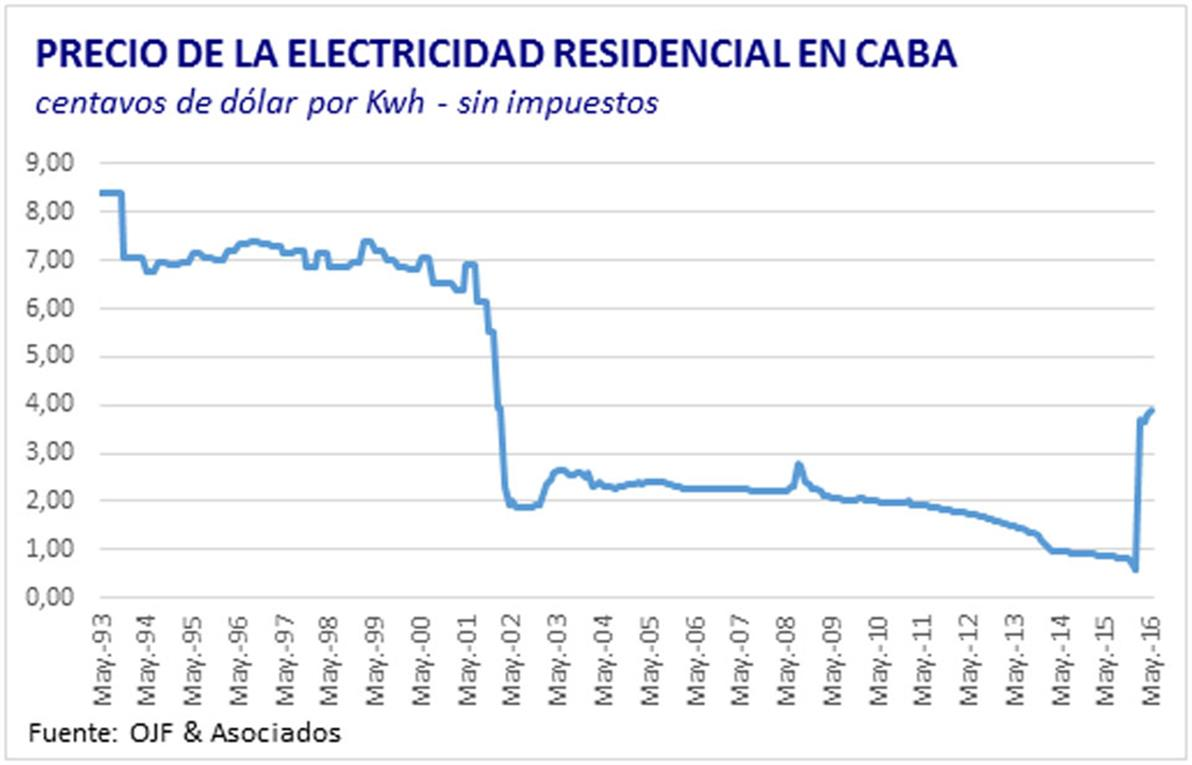
\includegraphics[width=12cm]{./Figures/1_1_costo_electricidad_caba.png}
	\caption{Evolución del costo de la energía eléctrica en la Ciudad Autónoma de Buenos Aires.}
	\label{fig:costo_caba}
\end{figure}

La preocupación de los consumidores se ve justificada en el hecho de que durante los primeros meses del año 2016 se produjo el primer aumento brusco en la tarifa, hecho que no ocurría desde hacía más de diez años. Y es en este contexto que se consideró importante desarrollar un producto que le permita al usuario conocer de una forma práctica y fácil la información del consumo de los aparatos eléctricos que utiliza cotidianamente. 

Y es importante destacar, que en la mayoría de los casos, la única información que posee el consumidor acerca de su consumo es la cantidad de energía consumida en un mes o en un bimestre por toda su instalación eléctrica. Contando con este único dato, es difícil poder tomar decisiones que modifican la forma de consumir energía eléctrica de las personas. El equipo propuesto en este trabajo buscó ofrecer una mayor información de cada dispositivo eléctrico al que se lo conecte. De esta forma, el usuario puede conocer en tiempo real las características del consumo de un aparato eléctrico.

Contando con información más detallada, el usuario:
\begin{itemize}
\item Identificar consumos de energía desconocidos.
\item Ajustar los horarios de funcionamiento del aparato eléctrico, adecuándolos a los momentos del día en el que realmente son necesarios.
\item Estimar el costo de  la energía consumida por cada aparato eléctrico.
\end{itemize}

Otro impulsor del proyecto fue que la disponibilidad local de equipos de automatización con estas características es extremadamente baja. Las soluciones que se comentan en la Sección \ref{section:soluciones_comerciales} pueden ser compradas a través de Internet, pero no de una forma sencilla en los comercios nacionales. Esta situación hace propicio el ofrecer una alternativa de fabricación nacional que pueda ser adquirida junto con otros productos que conformen una solución más completa de domótica.



\section{Soluciones comerciales existentes}
\label{section:soluciones_comerciales}

Actualmente, varias empresas a nivel mundial ofrecen productos para la automatización de cargas eléctricas. Comúnmente se denomina a estos equipos Smart Plugs y consisten básicamente en un equipo que se conecta al tomacorriente y al cual se conecta el aparato eléctrico que se quiere controlar. De esta forma, el Smart Plug queda conectado entre el tomacorriente y la carga eléctrica y permite:

\begin{itemize}
\item Encender y apagar la carga.
\item Conocer los parámetros eléctricos de la carga: tensión, corriente, factor de potencia, potencia activa, etc.
\item Informar la energía consumida por el aparato.
\item Programar horarios de encendido y apagado.
\item Monitorear la temperatura del equipo.
\end{itemize}

No todos los equipos comerciales cumplen con todas estas funcionalidades simultáneamente . Sin embargo, un punto común a todos los Smart Plugs comerciales es que ofrecen algún tipo de aplicación móvil para poder gestionar los Plugs dentro de una casa. Este aspecto es uno de los más importante en el diseño de un producto de estas características ya que la información que proveen los Smart Plugs debe ser mostrada al usuario de forma sencilla y útil para que pueda ser aprovechada.

Otra característica común es que muchos de los equipo son fabricados por empresas dedicadas a comercializar productos para redes de computadoras. De esta forma, se tienen algunos ejemplos como WeMo de la empresa Belkin, DS-W215 de D-Link y HS110 de TP-Link. En esta sección se describirán brevemente estos dos últimos equipos>

\begin{itemize}
\item \textbf{D-Link - DSP-W21}. Este dispositivo desarrollado por D-Link puede verse en la Figura \ref{fig:smartplug_dlink}. Las principales funciones que ofrece son: encendido/apagado de la carga tanto a través de la aplicación móvil como de un interruptor en el propio equipo, conexión a la red WiFi a través de WPS \footnote{WiFi Protected Setup. Es un conjunto de mecanismos que buscan facilitar la incorporación de un equipo a una red WiFi. Generalmente, para iniciar el proceso de WPS se debe presionar un botón en el producto que se desea incorporar a la red y se debe presionar el botón de WPS en el router WiFi. Una vez hecho esto el dispositivo se incorporará a la red.}, programación horaria del encendido/apagado y registro del consumo.

\begin{figure}[h]
	\centering
	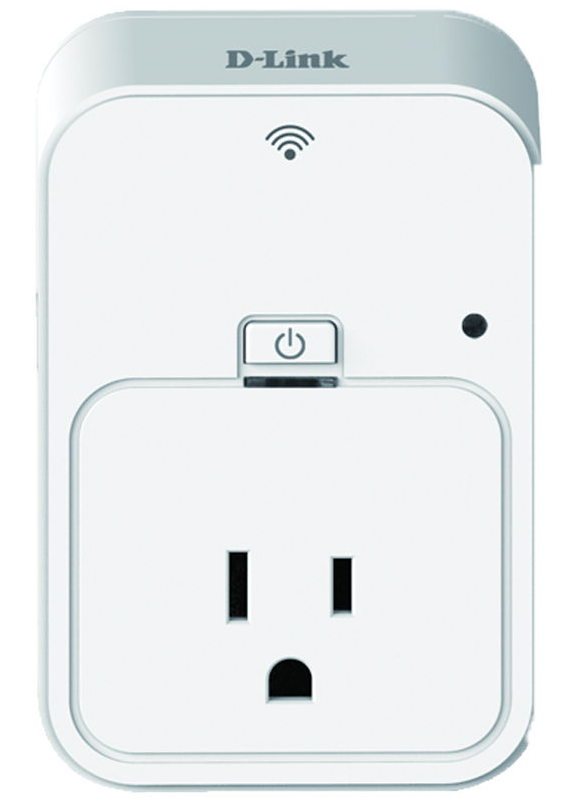
\includegraphics[width=6cm]{./Figures/1_2_DSP-W215.png}
	\caption{Smart Plug DSP-W215 de la empresa D-LINK}
	\label{fig:smartplug_dlink}
\end{figure}

La aplicación (disponible para dispositivos con sistema operativo Android y iOS) le permite al usuario controlar la carga desde la misma red WiFi en la que se encuentran los Smart Plugs y desde la red móvil. Esta aplicación también permite controlor otros productos de la línea  \textit{mydlink} como pueden ser cámaras y detectores de movimiento.

A diferencia de otros Smart Plugs, el gabinete es considerablemente grande (96 x 62 x 45 mm) lo cual es resaltado como un punto negativo en las reseñas de este producto.

Al momento de escribir esta memoria, el precio de este producto era de 50 dólares en Estados Unidos y no estaba disponible para ser adquirido en los comercios argentinos. Además, entre los tipos de enchufes disponibles para conectar la carga no se encuentra disponible el usado en Argentina.

\item \textbf{TP-Link - HS110}. Al igual que el anterior Smart Plug, el HS110 permite controlar una carga desde una aplicación móvil (disponible en Android y en iOS), pudiendo visualizar el tiempo total de encendido del dispositivo y la energía consumida tanto actual como en las semanas previas. Este producto ofrece un gabinete más reducido que el Smart Plug de D-Link. Puede verse una imagen del mismo en la Figura \ref{fig:smartplug_tplink}.

\begin{figure}[h]
	\centering
	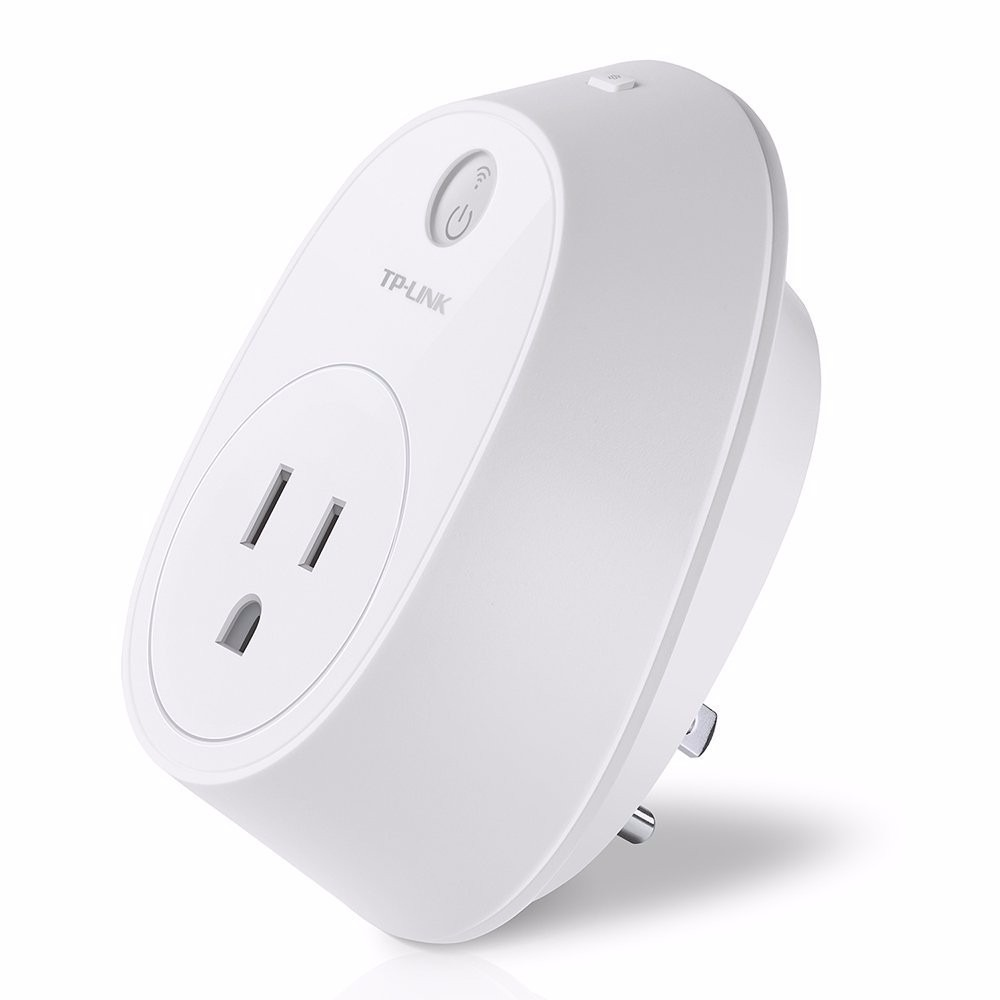
\includegraphics[width=6cm]{./Figures/1_2_TP-LINK-HS110.png}
	\caption{Smart Plug HS110 de la empresa TP-LINK}
	\label{fig:smartplug_tplink}
\end{figure}

Como diferencias con el producto de D-Link, se pueden mencionar que cada Smart Plug puede ser configurado para que se encienda y se apague de forma aleatoria para simular la presencia de una persona en el hogar.También es compatible con Amazon Echo, un producto que permite controlar dispositivos mediante comandos de voz.

El precio en Estados Unidos es cercano a los 40 dólares y al igual que el Smart Plug de D-Link no es vendido localmente.

\end{itemize}


\section{Objetivos}





%----------------------------------------------------------------------------------------







\chapter{Introducción Específica} % Main chapter title

\label{Chapter2}

%----------------------------------------------------------------------------------------
La idea de este capítulo es presentar una visión general del equipo desarrollado y mostrar algunos aspectos de la planificación del proyecto.


\section{Esquema general del sistema}

El producto básicamente debe permitir controlar una carga eléctrica a través de comandos que se le envían desde un teléfono móvil. Un esquema básico del sistema puede verse en la Figura \ref{fig:esquema_sistema}. Dentro del contexto de este trabajo final, se desarrolló un prototipo funcional de equipo. Por lo tanto es un producto que cumple todas la funciones que va a tener el equipo final, pero que no busca cumplir con características mecánicas y estéticas que si van a estar presentes en el producto comercial. Una descripción detallada del hardware desarrollado se encuentra en la Sección \ref{section:hardware}.

\begin{figure}[h]
	\centering
	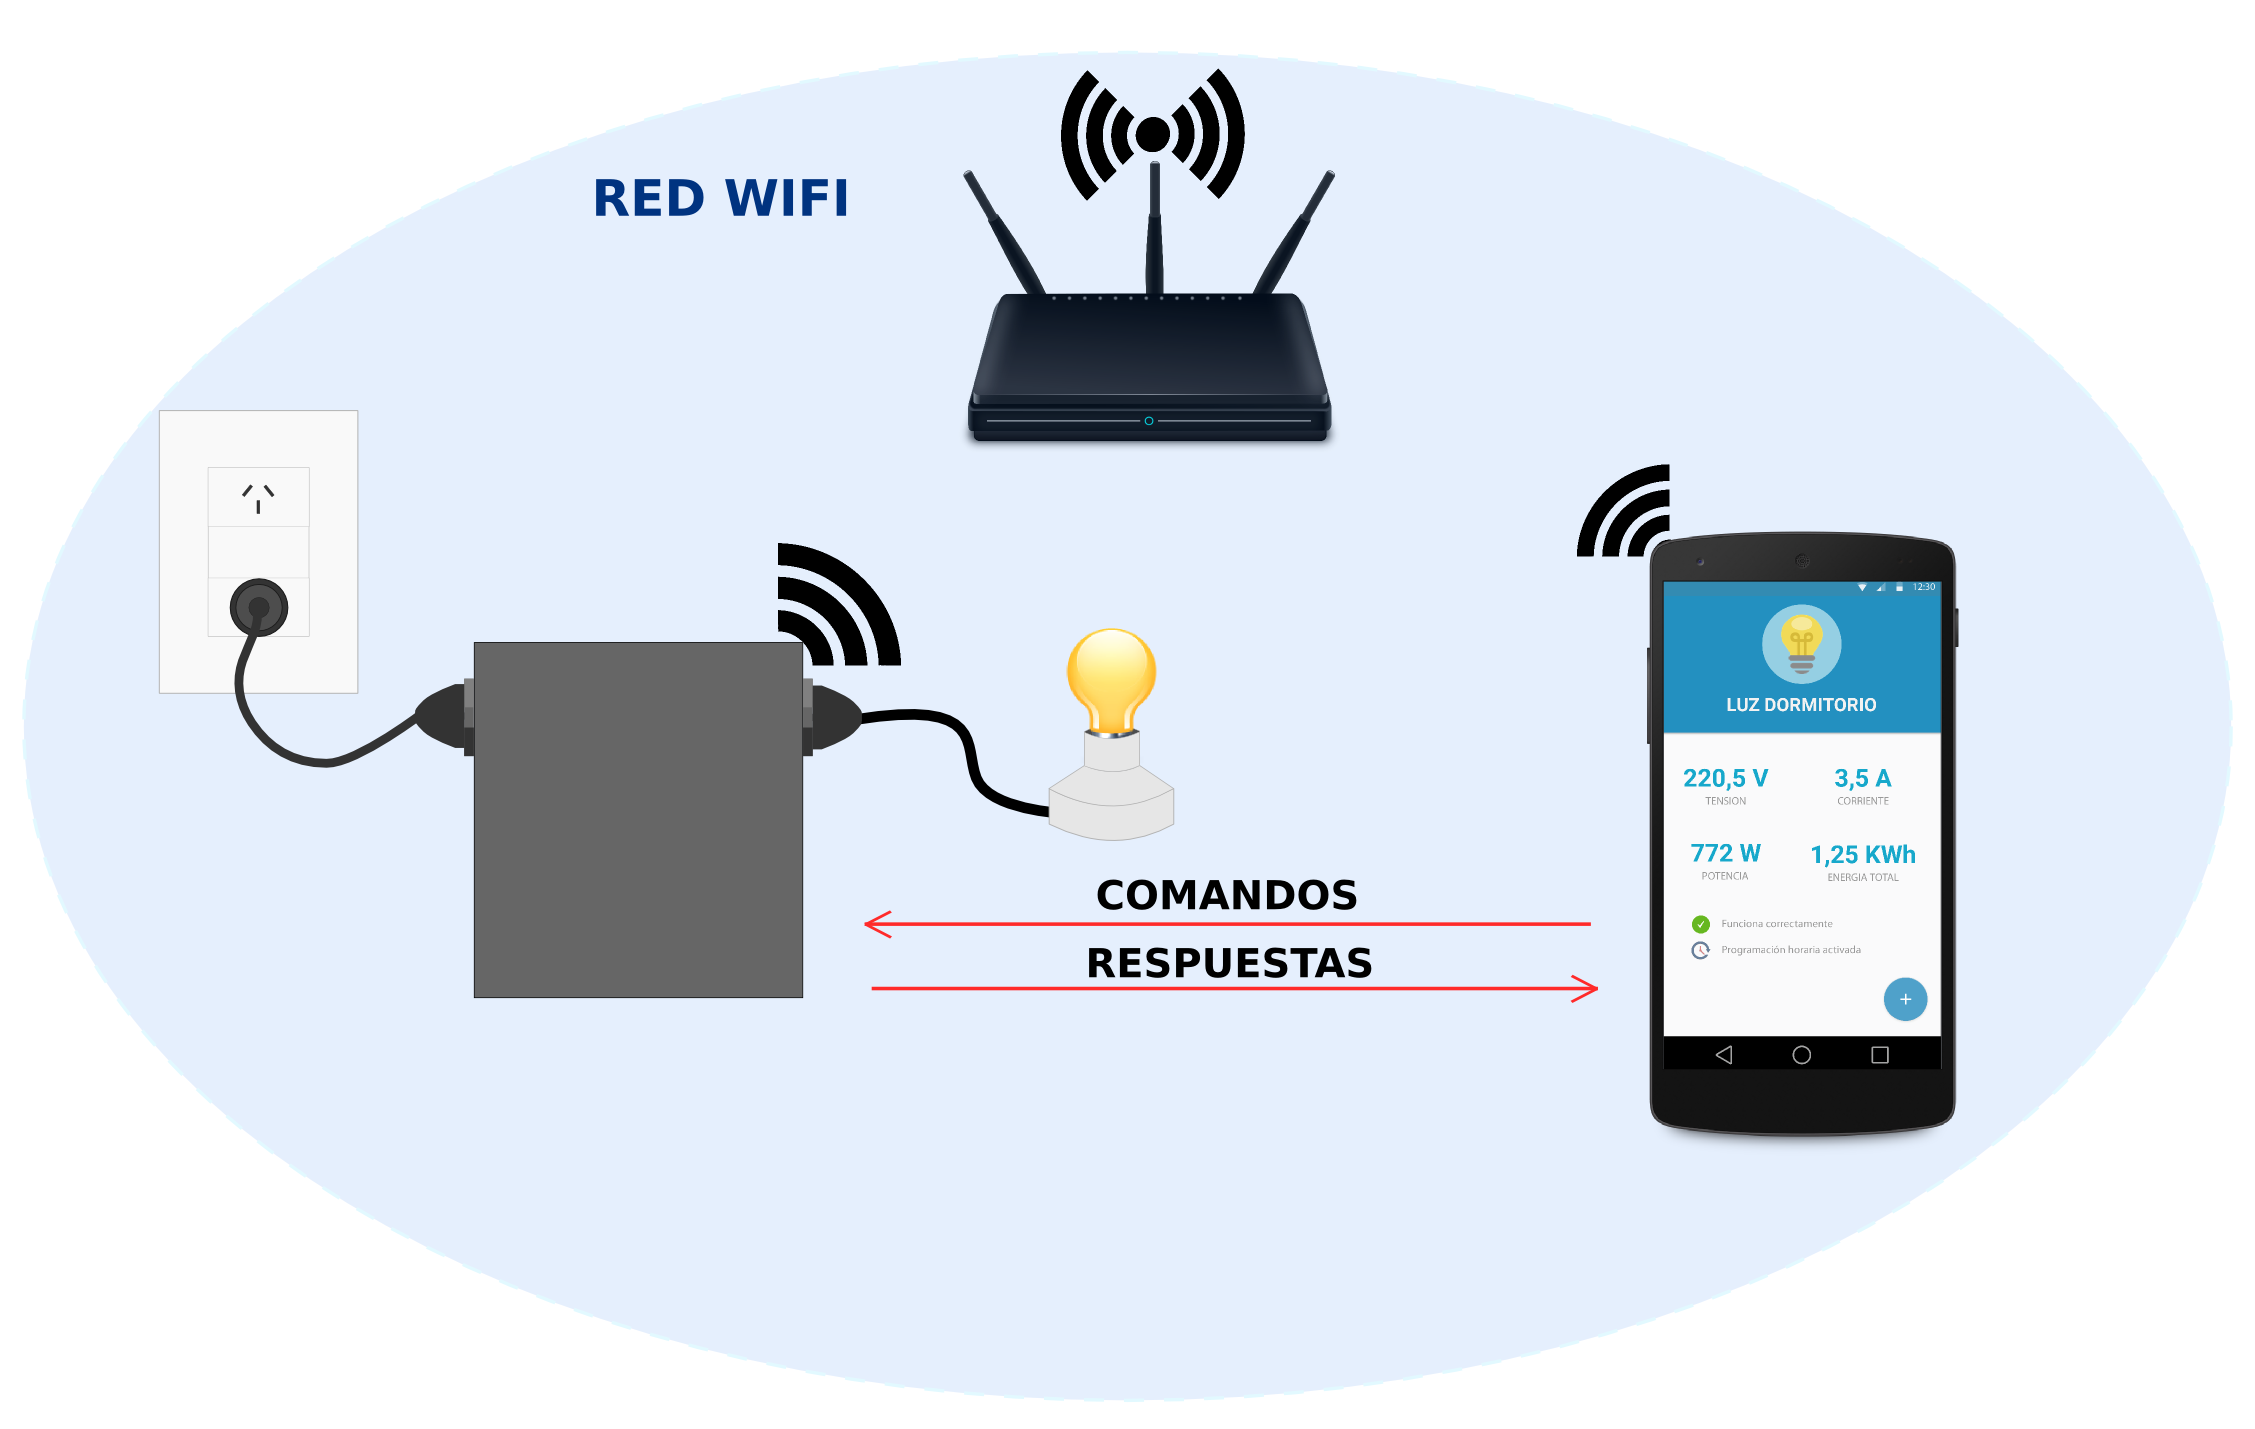
\includegraphics[width=12cm]{./Figures/2_1_esquema_sistema.png}
	\caption{Esquema general del sistema propuesto en este proyecto, compuesto por un Smart Plug y la aplicación móvil.}
	\label{fig:esquema_sistema}
\end{figure}

Cuando se adquiere un Smart Plug, lo primero que debe hacerse es incorporarlo a la red WiFi del hogar. Se eligió que la comunicación fuera a través de esta red, ya que con el paso de los años cada vez es más común que en las casas esté disponible este servicio, ya que muchos otros dispositivos electrónicos necesitan de una conexión a Internet.

Para agregar el Smart Plug a la red, se puede proceder de dos formas: WPS o configurando la red en el Smart Plug. En el primer caso, el proceso es sumamente sencillo: simplemente se debe presionar el pulsador que se encuentra en la placa del Smart Plug ( el led verde comenzará a destellar) y luego presionar el pulsador de WPS que se encuentra en el router WiFi. Una vez hecho esto, el Smart Plug se incorpora a la red. 

Sin embargo, muchos routers hogareños no cuentan con la funcionalidad de WPS, por lo que existe otra forma de configurar la red WiFi. Esta consiste en configurar el Smart Plug como un punto de acceso temporario. Para esto se debe mantener presionado el pulsador en la placa del Smart Plug durante 5 segundos. Cuando el led verde comienza a destellar, indica que el punto de acceso fue creado. Ahora se debe conectar un dispositivo móvil se debe conectar a la red WiFi creada por el Smart Plug. Una vez conectado, mediante un \textit{browser} se debe entrar ala página de configuración de la red WiFi (\textit{http://config}) y cargar los parámetros de la red a la que se desea conectar el Smart Plug: SSID de la red, tipo de seguridad y clave.

Cuando el Smart Plug se encuentra conectado a la red WiFi ya puede comenzar a ser comandado mediante la aplicación móvil. El único requerimiento para que el sistema funcione es que tanto los Smart Plugs como el teléfono en el que está la aplicación se encuentren en la misma red WiFi. En el alcance de este trabajo no estaba contemplada el desarrollo necesario de la infraestructura para poder comandar los Plugs desde fuera del hogar.

La aplicación lista todos los Plugs que encuentra en la red WiFi y permite: encender/apagar la carga, conocer algunos parámetros eléctricos de la carga (tensión corriente, potencia y energía), configurar horarios de encendido y apagado, visualizar mediciones históricas de potencia y energía. La cantidad de Smart Plugs que puede controlar la aplicación no está limitada, por lo que se pueden controlar numerosos dispositivos eléctricos dentro de una casa.

Además de poder enviar comandos a los Smart Plugs cuando el usuario lo requiere, la aplicación inicia un servicio en Android que se encarga de realizar consultas periódicamente a todos los Smart Plugs que tiene registrados, ún cuando la aplicación se encuentre cerrada. Mediante estas consultas, la aplicación va a poder conocer: si la carga está encendida o no, las últimas mediciones, los cambios en las configuraciones del equipo. De esta forma se logra que una aplicación móvil puedan comandar y configurar un Smart Plug y todas las demás que tengan registrado a ese mismo Plug se mantengan actualizadas con estos cambios. Una explicación más detallada del funcionamiento y del diseño de la aplicación móvil se encuentra en la Sección \ref{section:app}.

Finalmente, la comunicación entre los Smart Plugs y la aplicación móvil se basa en conexiones TCP iniciadas por la aplicación. Sobre TCP se desarrolló un protocolo propio que permite enviar comandos a los Plugs tanto para que realicen acciones como para leer/escribir valores de ciertos registros también definidos para este producto. Este protocolo es explicado en mayor profundidad en la Subsección \ref{subsection:protocolo}.



\section{Requerimientos}

A continuación se enumeran los requerimientos de hardware, firmware y de la aplicación móvil. Inicialmente se habían planteado un número mucho más reducido de requerimientos. Así también eran requerimientos que debían ser divididos en varios distintos para facilitar su validación. Antes de comenzar con el desarrollo del producto, se establecieron claramente los requerimientos. Para esto fueron importantes los aportes realizados desde las áreas de marketing (en cuanto al aspecto estético y funcionalidades deseadas) y de atención al cliente (en base a comentarios de los clientes referidos a un producto de estas características).

\begin{itemize}
\item Requerimientos de Hardware

\begin{itemize}
\item Req \#1.1: El Smart Plug debe poder operar con cargas de 220VAC y hasta 5A.
\item Req \#1.2: La fuente de alimentación debe generar 5V y 3,3V
\item Req \#1.3: La fuente de alimentación debe entregar 350mA.
\item Req \#1.4: El encendido y apagado de la carga se realizará con un relay mecánico de 5V. Se deben usar los contactos común y normal cerrado.
\item Req \#1.5: La interfaz de programación debe ser accesible mediante un header de pines.
\item Req \#1.6: Utilizar un front-end analógico monolítico para realizar el análisis de los parámetros eléctricos.
\item Req \#1.7: Conectarse a la red hogareña mediante un módulo WiFi.
\item Req \#1.8: Debe poseer un pulsador de tipo tact switch. El presionarlo pone un nivel lógico alto.
\item Req \#1.9: Debe poseer un led bicolor verde y rojo. Se encienden independientemente con un nivel lógico alto.
\item Req \#1.10: Deberá tener una memoria EEPROM SPI de la línea 25LC de Microchip.
\end{itemize}

\item Requerimientos de Firmware

\begin{itemize}
\item Req \#2.1: Cuando se inicia el modo WPS, el led verde debe destellar a una frecuencia aproximada de 1Hz.
\item Req \#2.2: Cuando se inicia el modo Soft-AP, el led verde debe destellar a una frecuencia aproximada de 2Hz.
\item Req \#2.3: Cuando se une a una red WiFi, si logra sincronizar la hora con el servidor NTP, el led verde se debe encender.
\item Req \#2.4: Cuando se une a una red WiFi, si no logra sincronizar la hora con el servidor NTP, el led verde y el rojo deben destellar.
\item Req \#2.5: Si no se puede unir a una red WiFi, el led rojo debe destellar a una frecuencia aproximada de 1Hz.
\item Req \#2.6: Al presionar el botón de la placa se debe iniciar el proceso de WPS.
\item Req \#2.7: Al mantener presionado por 5 segundos el botón de la placa se debe iniciar el Soft-AP.
\item Req \#2.8: Si se desconecta el Smart Plug, cuando se lo vuelve a conectar se debe intentar unir a la última red WiFi a la que estuvo unido.
\item Req \#2.9: Al conectarse a una red WiFi, se debe conectar a un servidor NTP y obtener la fecha y la hora.
\item Req \#2.10: La fecha y la hora deben ser llevadas por un RTC en el microcontrolador.
\item Req \#2.11: Debe existir un módulo encargado de registrar la actividad en el equipo. Su salida va a ser una UART configurada a 115200 baud - 8N1.
\item Req \#2.12: Se deben obtener las siguientes mediciones de la línea: tensión eficaz, corriente eficaz, potencia activa, frecuencia, factor de potencia y energía. 
\item Req \#2.13: El intervalo entre una muestra y la siguiente de cada medición no debe superar los 10 segundos.
\item Req \#2.14: Cada hora el Smart Plug debe obtener la potencia activa promedio de esa hora y la energía de esa hora.
\item Req \#2.15: Cada hora se deben guardar de forma no volátil las mediciones de potencia activa y energía correspondientes a esa hora.
\item Req \#2.16: Se deben guardar de forma no volátil las mediciones de potencia activa y energía correspondiente a las 24 horas de los últimos 7 días.
\item Req \#2.17: Cada dispositivo debe tener un ID único de 6 dígitos hexadecimales cargado durante la prueba de fábrica.
\item Req \#2.18: Cada dispositivo debe guardar de forma no volátil un nombre de hasta 32 caracteres.
\item Req \#2.19: Debe guardar de forma no volátil los parámetros de calibración del front-end analógico.
\item Req \#2.20: Debe permitir configurar una hora de encendido y apagado de la carga para cada día de la semana.
\item Req \#2.21: Cuando llega la hora de encendido configurada para el día correspondiente, la carga se debe encender.
\item Req \#2.22: Cuando llega la hora de apagado configurada para el día correspondiente, la carga se debe apagar.
\item Req \#2.23: Cuando el dispositivo se inicia debe chequear que la EEPROM esté inicializada. Debe haber un valor “bandera” en la EEPROM que indique si está inicializada.
\item Req \#2.24: Si la memoria EEPROM no está inicializada se deben cargar los siguientes valores: nombre - Smart Plug; horarios de encendido y apagado - 0:0.
\item Req \#2.25: El Smart Plug debe generar un mensaje UDP periódicamente para darse a conocer en la red WiFi. Lo debe enviar a la dirección broadcast.
\item Req \#2.26: En el mensaje periódico se debe indicar número de ID.
\item Req \#2.27: La comunicación con la App móvil va a ser a través de mensajes sobre TCP. Se debe respetar el formato de la trama definido en [1].
\end{itemize}

\item Requerimientos App móvil

\begin{itemize}
\item Req \#3.1: Debe identificar los Smart Plugs presenten en la red.
\item Req \#3.2: Debe permitir encender y apagar cada Smart Plug.
\item Req \#3.3: Debe mostrar el estado actual de la carga: encendida o apagada.
\item Req \#3.4: Debe mostrar el estado de la comunicación con cada Smart Plug: comunicación OK o con errores.
\item Req \#3.5: Debe mostrar la hora y la fecha de la última comunicación exitosa con cada Smart Plug. 
\item Req \#3.6: Debe permitir configurar el nombre de cada Smart Plug encontrado.
\item Req \#3.7: Debe permitir configurar el horario de encendido y apagado de la carga para cada día de la semana.
\item Req \#3.8: Debe permitir deshabilitar la programación horaria para cada día de la semana.
\item Req \#3.9: Debe permitir asignar un ícono a cada Smart Plug.
\item Req \#3.10: Debe permitir visualizar las mediciones de: tensión eficaz, corriente eficaz, potencia activa y energía acumulada. Para cada Smart Plug.
\item Req \#3.11: Debe permitir visualizar las mediciones históricas de potencia activa y energía de los últimos 20 días mediantes gráficos del tipo “Magnitud vs. hora del día”.
\item Req \#3.12: Debe permitir borrar las mediciones históricas y la energía acumulada en los Smart Plugs.
\item Req \#3.13: Debe permitir volver a valores de fábrica a los Smart Plugs.
\item Req \#3.14: Debe actualizar de forma periódica (cada 10 minutos) la información de cada Smart Plug. La información incluye: nombre del dispositivo, estado de la carga, tensión eficaz, corriente eficaz, potencia activa y energía acumulada.
\item Req \#3.15: Debe actualizar de forma periódica (cada 1 hora) las mediciones por hora de la potencia activa y energía de cada Smart Plug.
\item Req \#3.16: La actualización periódica debe continuar aún cuando la aplicación esté cerrada.
\end{itemize}

\end{itemize}



\section{Planificación}

En la Figura \ref{fig:diagrama_gantt} puede observarse el diagrama de Gantt con la tareas realizadas en el contexto de este proyecto.

\begin{figure}[!h]
	\centering
	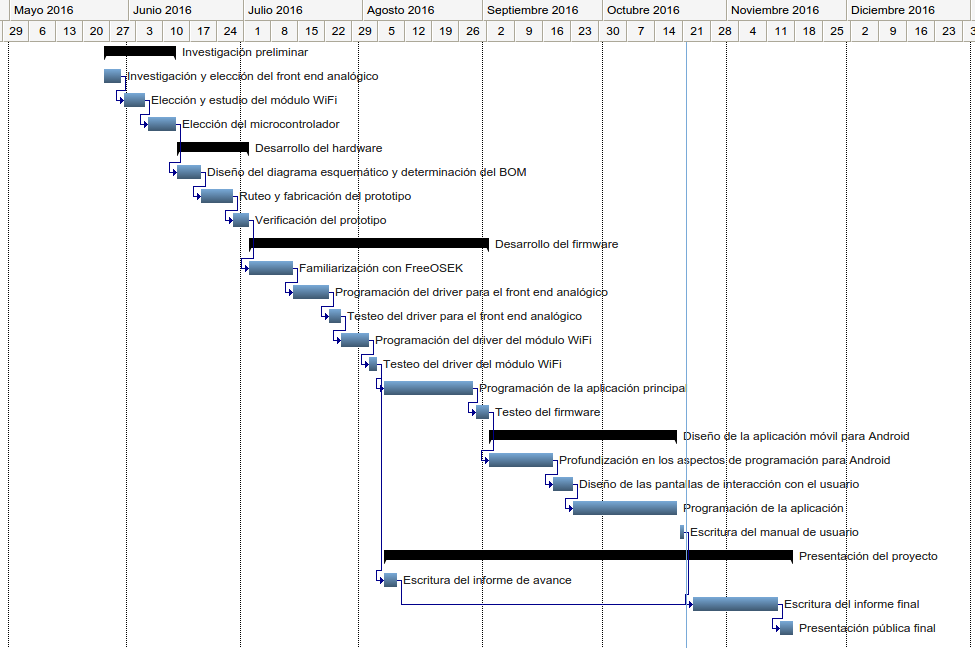
\includegraphics[width=18cm, angle=90]{./Figures/2_3_diagrama-Gantt.png}
	\caption{Diagrama de Gantt de la planificación del proyecto.}
	\label{fig:diagrama_gantt}
\end{figure}


Para mayor información acerca de la planificación se puede recurrir al documento \textit{Planificación del Trabajo Final de Carrera - Mondani Mariano} en \citep{repo_planificacion}, en donde se puede encontrar la planificación detallada, incluyendo las tareas y los riesgos que se contemplaron al iniciar el proyecto.
 
\chapter{Diseño e Implementación} % Main chapter title

\label{Chapter3} % Change X to a consecutive number; for referencing this chapter elsewhere, use \ref{ChapterX}
\definecolor{mygreen}{rgb}{0,0.6,0}
\definecolor{mygray}{rgb}{0.5,0.5,0.5}
\definecolor{mymauve}{rgb}{0.58,0,0.82}

%----------------------------------------------------------------------------------------

La idea de este capítulo es explicar los criterios utilizados en el desarrollo del producto y justificar las decisiones de diseño; así como también explicar el detalle de la implementación de los distintos aspectos del producto.

\section{Hardware}
\label{section:hardware}

En el contexto del presente trabajo, se desarrolló un prototipo funcional del producto final. Este prototipo presenta las mismas funciones que el equipo final pero no se ajusta a los lineamientos estéticos y mecánicos que si deberá cumplir el producto. Es por esto que el prototipo diseñado tiene dimensiones mucho más grandes que las que tendrá, lo cual facilitó las mediciones y pruebas que se debieron realizar para comprobar el correcto funcionamiento tanto del hardware como del firmware. 

En la Figura \ref{fig:prototipo} puede verse una fotografía del prototipo. En la misma se puede apreciar el PCB diseñado y las dos conexiones principales: a la izquierda del gabinete la conexión a la línea eléctrica y a la derecha la conexión a la carga eléctrica. La placa fue colocada dentro de un gabinete que por supuesto no tiene relación alguna con el gabinete que finalmente se utilizará. Simplemente cumple la función de facilitar la manipulación del prototipo.

\begin{figure}[h]
	\centering
	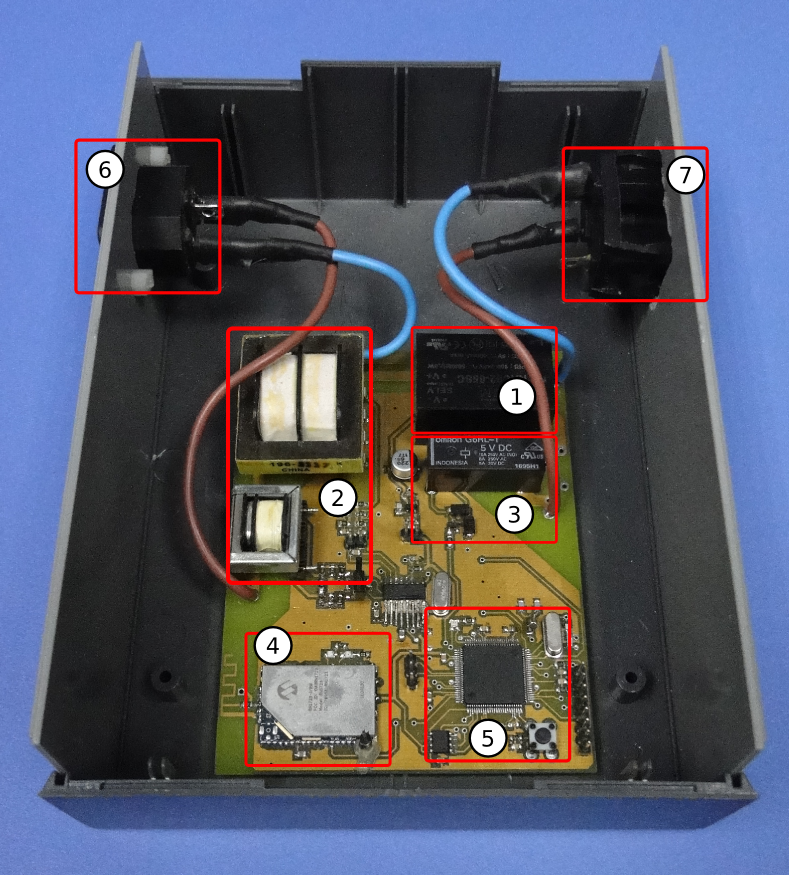
\includegraphics[width=11cm]{./Figures/3_1_prototipo_1.png}
	\caption{Prototipo funcional del Smart Plug. 1 - Fuente de alimentación. 2 - Adaptación de las señales de línea. 3 - Control de la carga. 4 - Módulo WiFi. 5 - Microcontrolador, led bicolor, pulsador y memoria EEPROM. 6 - Conexión a la línea eléctrica. 7 - Conexión a la carga.}
	\label{fig:prototipo}
\end{figure}

Los bloques mencionados en la Figura \ref{fig:prototipo} son explicados en las Subsecciones \ref{subsec:esquematico_general} y \ref{subsec:detalles_hardware}.

A pesar de ser un prototipo funcional, el hardware se diseño pensando en las caracteríticas finales que tendrá el producto. Por lo tanto se debieron definir las especificaciones deseadas para el equipo:

\begin{itemize}
\item Tensión máxima de operación: 240VAC
\item Corriente máxima de operación: 5A
\end{itemize}

Para una tensión de operación de 220VAC, la máxima potencia que se puede conectar es de 1100W. Para un primer producto se buscó cubrir la automatización de aparatos eléctricos de baja potencia como lámparas, ventiladores, electrodomésticos pequeños, televisores, etc. El manejo de equipos de mayor potencia como aires acondicionados, estufas eléctricas, hornos eléctricos, etc, será cubierto en un futuro cuando se modifique el hardware para soportar una mayor corriente, generando así un nuevo producto.



\subsection{Esquemático general}
\label{subsec:esquematico_general}

En la Figura \ref{fig:hardware_diagrama_bloques} pueden verse los principales bloques funcionales del prototipo.

\begin{figure}[h]
	\centering
	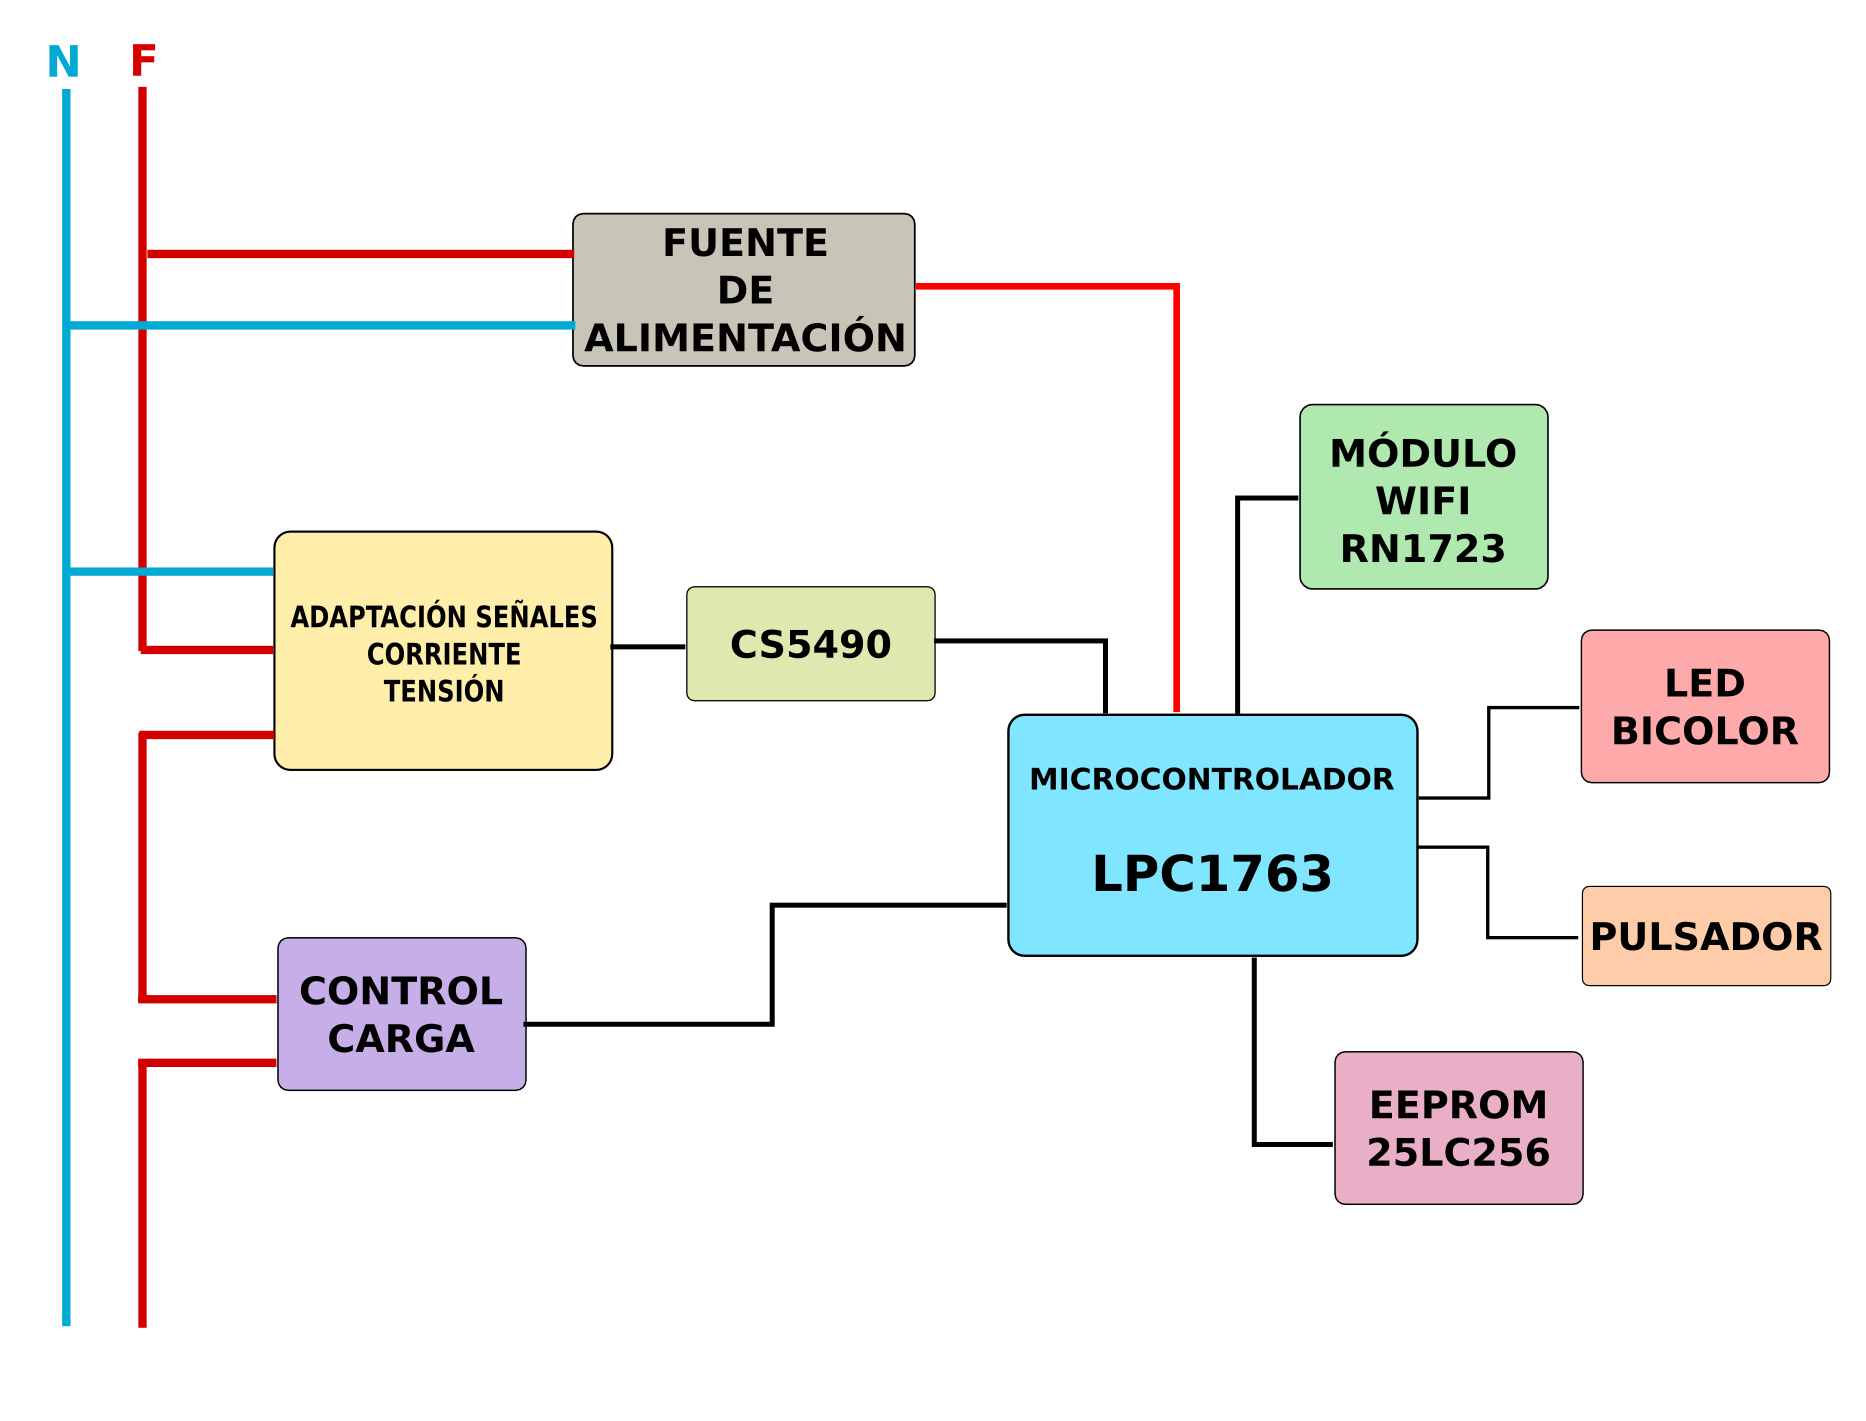
\includegraphics[width=12cm]{./Figures/3_1_1_diagrama_bloques_hardware.png}
	\caption{Diagrama en bloques del hardware del prototipo funcional.}
	\label{fig:hardware_diagrama_bloques}
\end{figure}

A continuación se describe brévemente cada uno de los módulos. Una explicación más detallada de cada uno se encuentra en la Subsección \ref{subsec:detalles_hardware}:

\begin{itemize}
\item Fuente de alimentación. La alimentación del equipo es obtenida de la misma línea eléctrica a la que está conectado el dispositivo. Debe generar dos niveles de tensión, 5V y 3,3V y debe ser capaz de entregar soportar el consumo especialmente del módulo WiFi.
\item Adaptación de las señales de corriente y tensión. Este bloque se encarga de adaptar la señal de tensión de la línea y la señal de la corriente consumida por el aparato eléctrico a los niveles que requiere el front-end analógico CS5490. La adaptación se realiza mediante transformadores para lograr una completa aislación de la línea.
\item Front-end analógico CS5490. Es el circuito integrado encargado de tomar las señales de la línea y generar las mediciones eléctricas de interés: tensión eficaz, corriente eficaz, frecuencia de línea, factor de potencia, energía consumida, etc.
\item Control de la carga. La conmutación de la carga se realiza mediante un relay mecánico.
\item Módulo WiFi RN1723. Es el módulo encargado de permitir la comunicación entre el Smart Plug y la aplicación móvil. Básicamente se encarga de esperar conexiones TCP y enviar las respuestas requeridas al socket del que provino el comando.
\item Microcontrolador LPC1763. Es el encargado de implementar la lógica del Smart Plug. 
\item Memoria EEPROM. Es la encargada de retener información de configuración del Smart Plug y las mediciones diarias de potencia y energía.
\item Led bicolor. Es un led rojo y verde encargado de realizar las señalizaciones acerca del funcionamiento del equipo. En la Subsección \ref{sec:validacion_firmware} se describe el significado de las distintas señalizaciones.
\item Pulsador. Mediante el pulsador se inician loas procesos destinados a incorporar el Smart Plug a la red WiFi de la casa.
\end{itemize}

\subsection{Descripción de los módulos de hardware}
\label{subsec:detalles_hardware}

En este apartado de la memoria se describen las decisiones de diseño asociadas a los módulos de hardware. Los fragmentos de esquemático que a continuación se muestran surgen del archivo \textit{SmartPlug\_v1.0} en \citep{repo_hardware}.

\subsubsection{Fuente de alimentación}

El esquemático de la fuente del Smart Plug puede verse en la Figura \ref{fig:pcb_fuente}. Esta fuente de alimentación se conecta a la misma línea eléctrica que es medida por el front-end analógico. A partir de la tensión de 220VAC genera una tensión de 5V y 3,3V. Para lograr los 5V se utiliza una fuente switching con montaje para PCB VSK-S2-5U la cual puede entregar hasta 400mA. Esta fuente permite generar una tensión estable manteniendo un empaquetado de reducido tamaño (34 x 22 x 18 mm). 

\begin{figure}[h]
	\centering
	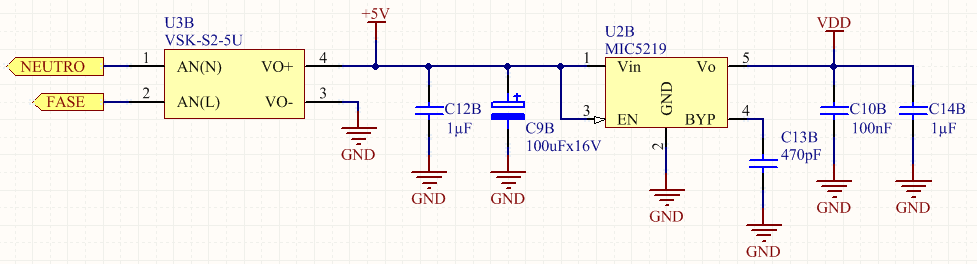
\includegraphics[width=14cm]{./Figures/3_1_2_pcb_fuente.png}
	\caption{Esquemático de la fuente de alimentación.}
	\label{fig:pcb_fuente}
\end{figure}


Se debe aclarar que esta switching fuente fue elegida para el prototipo funcional. En la versión final del equipo se utilizará una fuente switching AC-DC de similares características diseñada dentro de la empresa, debido a que tanto el tamaño del empaquetado de la fuente como su costo (U\$s 13,25 por unidad al momento de escribir la memoria) son prohibitivos para incluir esta fuente en el diseño final.

En cuanto al regular de 3,3V se eligió un componente que puede entrgar hasta 500mA. El requerimiento de corriente tanto de la fuente switching como del regulador de 3,3V surge del consumo especialmente del módulo WiFi RN1723, el cual puede consumir hasta 250mA.


\subsubsection{Adaptación de las señales de tensión y corriente}

En la Figura \ref{fig:pcb_adaptacion} puede verse la sección del esquemático relacionada con la adaptación de las señales de tensión y de corriente del dispositivo. Para poder obtener las mediciones eléctricas y el consumo de la carga conectada al Smart Plug es necesario adaptar las señales de tensión de línea y de la corriente consumida por la carga a los niveles soportados por el front-end analógico.

\begin{figure}[h]
	\centering
	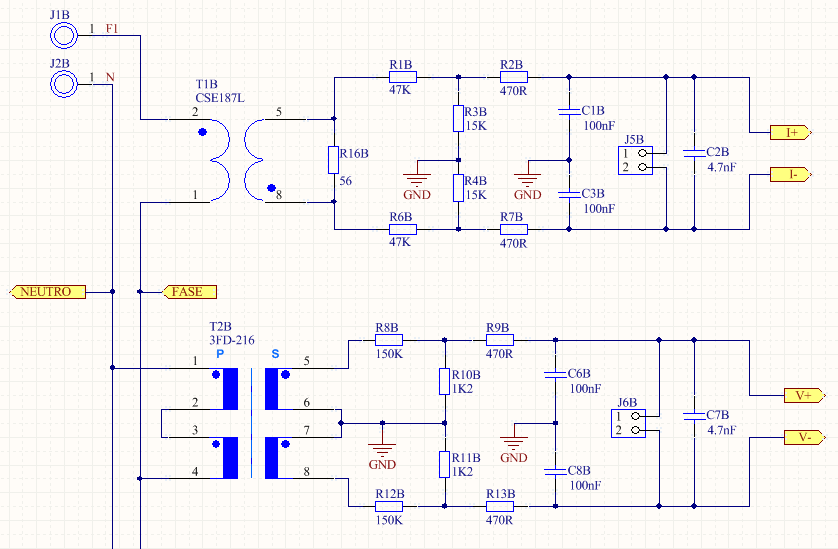
\includegraphics[width=14cm]{./Figures/3_1_2_pcb_adaptacion.png}
	\caption{Esquemático de la etapa de adaptación de las señales de tensión y corriente de la línea eléctrica.}
	\label{fig:pcb_adaptacion}
\end{figure}

De acuerdo a la hoja de datos del front-end elegido para este proyecto (CS5490) tanto la señal de corriente como la de tensión no deben superar los 250mV de pico en las entradas diferenciales del circuito integrado. Para lograr esto, primero se debe definir la tensión y la corriente máxima que debe medir el Smart Plug. En el caso concreto de este proyecto, y como ya fue mencionado, estos valores son: tensión máxima - 240VAC, corriente máxima - 5A.

Definidos estos valores, se eligió aislar el resto del circuito de la línea eléctrica tomando las señales de tensión y corriente mediante transformadores. Al igual que sucedió con la elección de la fuente switching, esta decisión fue exclusivamente para el desarrollo del prototipo funcional, ya que en la versión final será conveniente reemplazar el transformador de tensión por divisores resistivos y el transformador de corriente por un shunt. Ambos cambios van a permitir reducir el tamaño del producto final y su costo.

Luego de los transformadores hay divisores resistivos dispuestos en forma diferencial para reducir la tensión a los valores tolerados por el CS5409. Finalmente hay filtros pasa-bajo con un a frecuencia de corte de 3,3kHz.

Con los valores elegidos de relación de transformación y divisores resistivos, los valores máximos soportados por el equipo resultan:

\begin{itemize}
\item Tensión máxima soportada por el hardware: 320VAC.
\item Corriente máxima soportada por el hardware: 6,5A.
\end{itemize}

Ambos valores se encuentran por encima de los valores máximos informados al usuario.


\subsubsection{Front-end analógico}

Luego de adaptar las señales de tensión y de corriente, las mismas deben ser medidas por un front-end analógico que se encargará de generar los parámetros de interés para la aplicación: tensión y corriente eficaz, frecuencia de línea, potencia activa, factor de potencia, energía consumida, etc. En la Figura \ref{fig:pcb_medicion_energia} puede verse l circuito asociado al front-end elegido, el CS5490.

\begin{figure}[h]
	\centering
	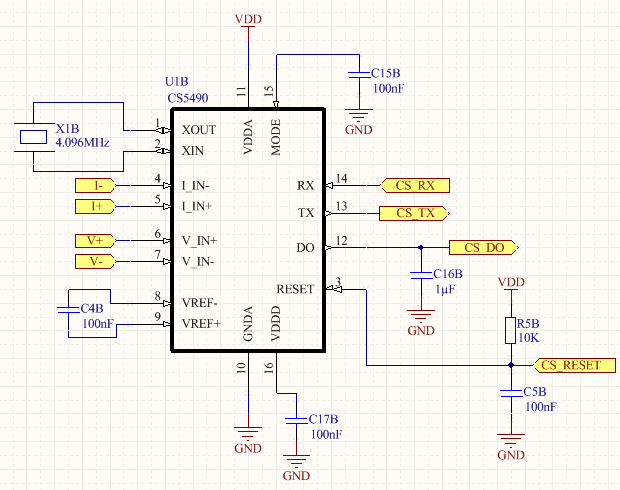
\includegraphics[width=14cm]{./Figures/3_1_2_pcb_medicion_energia.png}
	\caption{Esquemático del front-end analógico encargado de medir los parámetros eléctricos.}
	\label{fig:pcb_medicion_energia}
\end{figure}

A parte de los componentes relacionados con la adaptación de las señales de línea, este circuito integrado  no necesita de una gran cantidad de componentes adicionales, salvo algunos capacitores y un cristal de 4,096Mhz con el cual va generar la base de tiempo interna para realizar las mediciones y cálculos.

La comunicación es sencilla, a través de comandos enviados por una UART. Con estos comandos se van poder conocer casi todas las mediciones que calcula el CS5490. La única medición que no puede ser conocida a través de la lectura de un registro es la energía consumida. Esta es informada mediante pulsos a través del pin \textit{DO}. Se debe configurar la constante del medidor en el CS5490, es decir la cantidad de pulsos a los que equivale un kilowatt-hora.


\subsubsection{Control de la carga}

La conmutación de la carga está a cargo de un relay mecánico. En la Figura \ref{fig:pcb_control_carga} puede verse que la fase de la línea eléctrica se conecta entre los contactos \textit{común} y \textit{normal cerrado} del relay para que, en caso de ocurrir un desperfecto con el Smart Plug, la carga pueda seguir funcionando.

\begin{figure}[h]
	\centering
	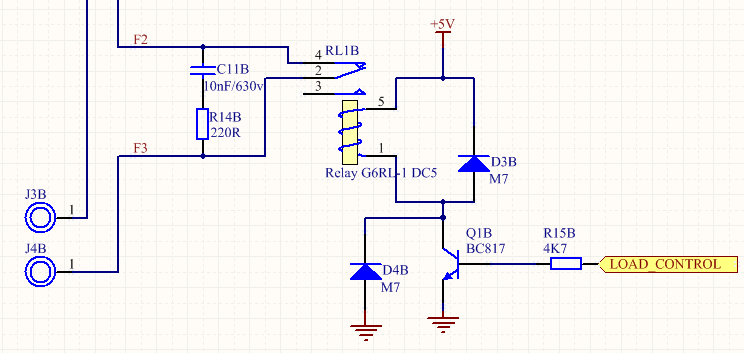
\includegraphics[width=10cm]{./Figures/3_1_2_pcb_control_carga.png}
	\caption{Esquemático del control de la carga eléctrica mediante un relay mecánico.}
	\label{fig:pcb_control_carga}
\end{figure}

Para funcionar, la bobina del relay requiere de una tensión de 5V y los contactos soportan una corriente máxima de 8A con 250VAC, valor que satisface sobradamente las especificaciones propuestas para el Smart Plug.

\subsubsection{Módulo WiFi}

El módulo elegido es el RN1723, el cual prácticamente no requiere de componentes adicionales y se comunica con el microcontrolador mediante una UART.

Para la antena del módulo se eligió una antena impresa en el PCB de acuerdo a las especificaciones de la hoja de datos del módulo.

Al momento de comenzar con el proyecto y elegir los componentes, este módulo resultaba una opción atractiva, que proveía las funcionalidades especificadas en los requerimientos del producto a un precio aceptable. Además se decidió elegir este módulo ya que es comercializado por Microchip, marca que es ampliamente usada por los productos de X-28 Alarmas, lo cual lleva a la posibilidad de obtener precios muy competitivos con los distribuidores.

\section{Firmware}

\subsection{Arquitectura del firmware}

El firmware embebido en el Smart Plug se escribió utilizando FreeOSEK como sistema operativo de tiempo real. De esta forma, en la Figura \ref{fig:firmware_esquema_tareas} pueden verse las tareas que se crearon y la interacción que entre estas.

Básicamente, las características del firmware surgen de los requerimientos enumerados en la Sección \ref{sec:requerimientos} y son:

\begin{itemize}
\item Iniciar el proceso de WPS o configurarse en modo punto de acceso (AP) cuando se presiona el pulsador presente en la placa.
\item Mostrar el estado del dispositivo a través del led bicolor.
\item Escuchar las conexiones TCP que provengan de las aplicaciones móviles y generar las respuestas adecuadas.
\item Guardar de forma no volátil (en la memoria EEPROM) la potencia activa promedio y energía consumida de cada hora del día. En la EEPROM se guarda la información de los últimos 7 días.
\item  Sincronizar la hora del Smart Plug con un servidor NTP y gestionar el encendido y apagado de la carga de acuerdo a la programación horaria configurada.
\end{itemize}

\begin{figure}[h]
	\centering
	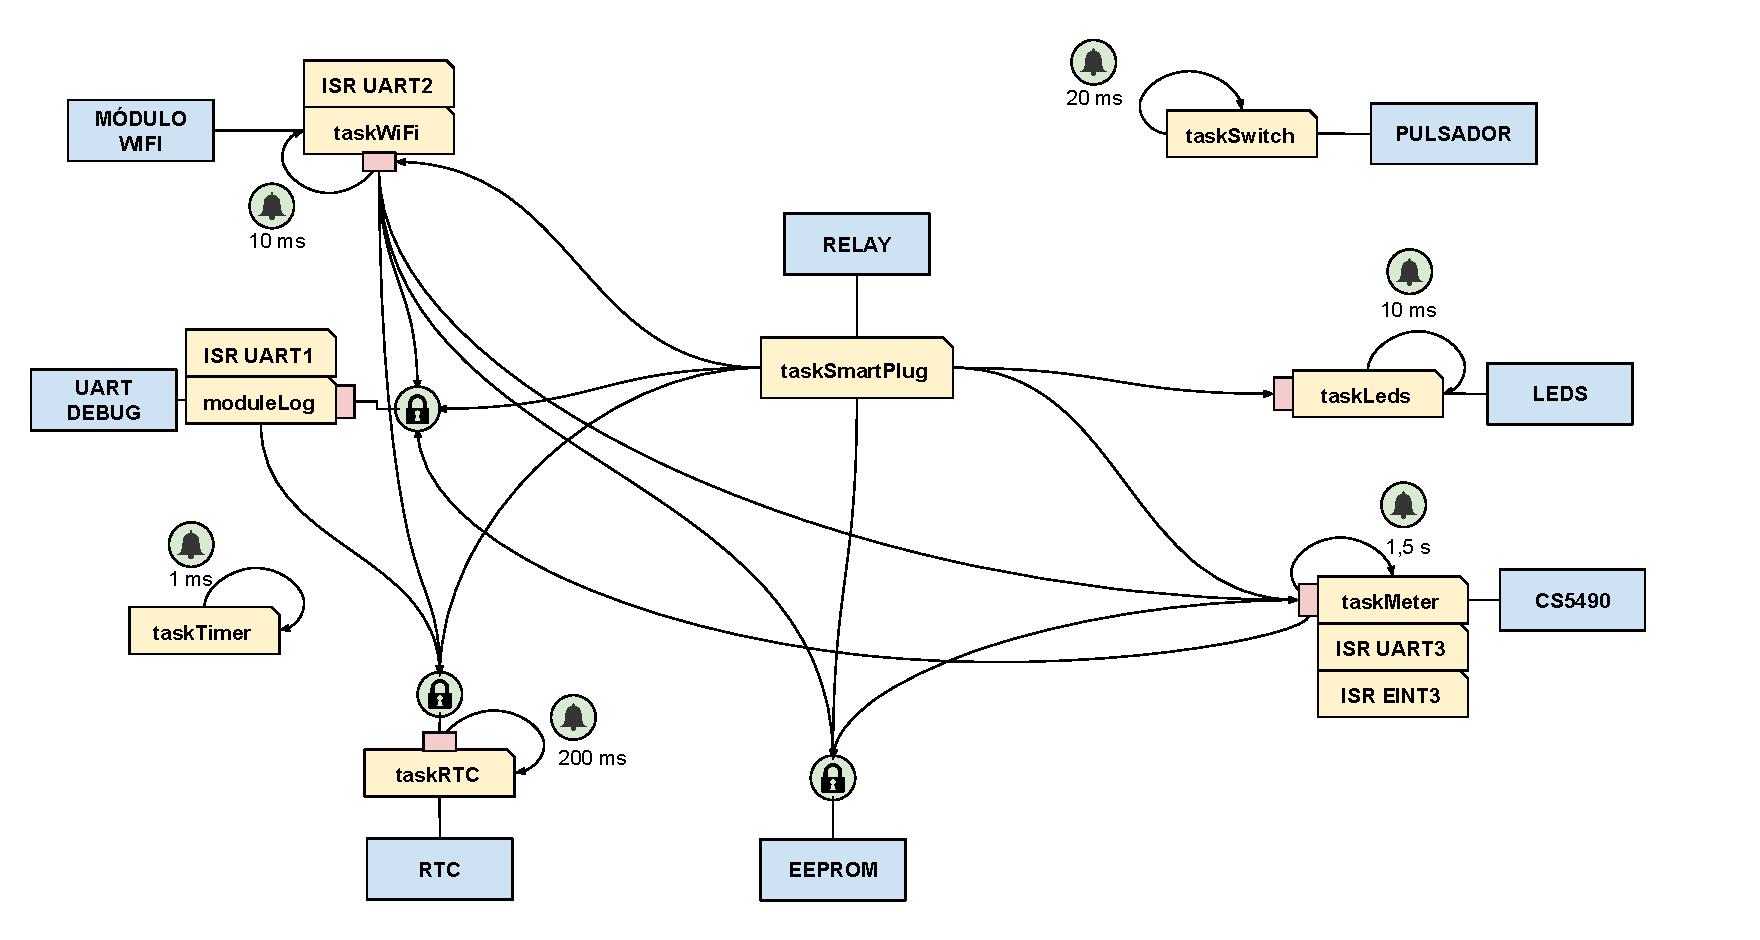
\includegraphics[width=16cm]{./Figures/3_2_1_firmware_esquema_tareas.pdf}
	\caption{Esquema de las tareas y recursos utilizados en el firmware.}
	\label{fig:firmware_esquema_tareas}
\end{figure}

A continuación se describe cada una de las tareas:

\begin{itemize}
\item taskSmartPlug. Es la tarea principal del Smart Plug. Se encarga de implementar la lógica del dispositivo. Se encarga de recibir los eventos generados por el resto de las tareas y realizar acciones en base a los mismos. Se va a bloquear esperando que ocurra alguno de los eventos. 

De taskWiFi obtiene los eventos relacionados con la conexión a la red WiFi y las conexiones TCP. Además le indica cuando tiene que iniciar un proceso de WPS o configurarse como punto de acceso.

A taskLeds le indica la señalización que debe realizar de acuerdo al evento recibido. En la Tabla \ref{tab:senializacion_leds} puede verse un resumen de todas las posibles señalizaciones.


De taskMeter obtiene las últimas mediciones para guardarlas de forma no volátil en la memoria EEPROM e ir generando un registro de potencia activa y energía consumida por hora de los últimos 7 días.

Además se encarga de manejar el relay que conmuta la carga eléctrica. El encendido o apagado de la misma se va a determinar a partir de la programación horaria (si está configurada) y de los comandos de encendido y apagado que envíe la aplicación móvil.

\item taskSwitch. Gestiona el pulsador de tipo tact switch que se encuentra en el PCB. Realiza el anti-rebote y genera los eventos cuando es presionado. Va a generar un evento cuando se suelte el pulsador (lo cual inicia el proceso de WPS en el módulo WiFi) y otro cuando se mantenga presionado por más de 5 segundos (lo cual configura al módulo WiFi como un punto de acceso). 

Es una tarea que se ejecuta cada 20ms mediante una alarma de FreeOSEK.


\item taskLeds. Se encarga de realizar las señalizaciones indicadas por otras tareas. Las señalizaciones se forman a partir de un led bicolor (rojo y verde), tanto encendiéndolos, apagándolos o haciéndolos destellar a distintas frecuencias.
Es una tarea periódica que se ejecuta cada 10ms, mediante una alarma de FreeOSEK, para actualizar los leds.


\item taskRTC. Se encarga de configurar y acceder al RTC interno del microcontrolador. Es la tarea que genera los eventos para indicar el paso de un minuto, una hora o un día, los cuales son utilizados por taskSmartPlug para registrar las mediciones de potencia activa y energía consumida por hora.

\item taskWiFi. Se encarga de recibir las conexiones desde la aplicación móvil. Interacciona con taskMeter para requerir las últimas mediciones de acuerdo a lo solicitado por la aplicación móvil.

También consulta la memoria EEPROM para leer o modificar los parámetros de configuración del Smart Plug y para enviarle a la aplicación móvil las mediciones históricas de potencia activa y energía consumida.

Cuando se inicia la tarea se conecta con un servidor NTP para obtener la fecha y hora. Estos parámetros son enviados a la tarea taskRTC para que configure el RTC interno del microcontrolador.

La comunicación con el módulo es a través de una UART y tanto la recepción como la transmisión se realizan a través de la interrupción de este periférico. La tarea es periódica, cada 10ms para controlar los mensajes que llegan desde el módulo RN1723  de forma asincrónica.

\item taskMeter. Se encarga de obtener periódicamente las mediciones del front-end analógico CS5490. Además acumula los pulsos generados por el mismo integrado para llevar un registro de la energía consumida por la carga.

Al iniciar la tarea, se encarga de configurar el CS5490 para que funcione de acuerdo a lo especificado. Este proceso incluye:

\begin{itemize}
\item Configurar la constante del meidor. Es la cantidad de pulsos a los que va a equivaler un kilowatt-hora. Para este proyecto se eligió una constante de 5000 pulsos/kWh. Esta constante no es configurada directamente en el CS5490, sino que se deben escribir algunos registros del integrado para lograr que genere 5000 pulsos por kWh. El proceso para lograr esto está explica en la Sección 5.5 de \citep{datasheet_CS5490}.
\item Configurar la tensión y corriente máxima de operación, ya que las mediciones van a ser calculadas a partir de estos parámetros.
\item Cargar los valores de calibración. Para lograr los valores de error relativo en el canal de tensión y de corriente que informa la hoja de datos es necesario realizar un proceso de calibración del equipo. Básicamente este proceso consta de dos etapas: calibración de \textit{offset} de continua y calibración de ganancia. Para el primero se deben cortocircuitar las entradas diferenciales del canal de tensión y de corriente y comenzar el proceso. Para la calibración de ganancia, en el caso de la tensión, se debe generar la tensión máxima que puede medir el Smart Plug y comenzar el proceso de calibración. Para el caso de la corriente, se puede usar una corriente menor a la máxima del Smar Plug que debe ser indicada al CS5490 antes de comenzar con la calibración.
Este proceso se encuentra detalladamente explicado en la Sección 7.1 de \citep{datasheet_CS5490}.

En el contexto del presente trabajo el proceso de calibración no se incluyó. Los valores de calibración se calcularon y luego se ajustaron manualmente. En la Sección \ref{sec:trabajo_futuro} se propondrá una posible forma de implementar la etapa de calibración en el proceso de fabricación del producto final.
\end{itemize}

La comunicación con el CS5490 se realiza a través de una UART y tanto la recepción como la transmisión se realizan a través de la interrupción de este periférico. Además se utiliza otra interrupción, encargada de detectar los pulsos generados por el CS5490 apra indicar la energía consumida.
Es una tarea periódica.

\item moduleLog. Es la tarea encargada de enviar información de la actividad de la aplicación a través de mensajes por una UART. Otras tareas le envían mensajes que debe sacar por la UART, incluyendo la fecha y la hora en la que se produjo el mensaje. Esto tuvo una especial importancia al momento de desarrollar el firmware para conocer los eventos que se estaban produciendo. Los mensajes son enviados a una velocidad de 115200 baudios y se debe conectar un adaptador TTL-USB en la tira de pines destina a la UART en el PCB (llamada DEBUG en el esquemático).

\end{itemize}


\begin{table}[h]
	\centering
	\caption[Señalizaciones del Smart Plug]{Señalizaciones del Smart Plug a través del led bicolor.}
	\begin{tabular}{c c c c c}    
		\toprule
		\textbf{Señalización} 	 & \textbf{Modo AP}  & \textbf{Modo WPS}  & \textbf{Autenticado}  & \textbf{RTC Sincronizado} \\
		\midrule
		Verde destella a 2Hz	 	& 1  & X  & X  & X \\		
		Verde destella a 1Hz	 	& 0  & 1  & X  & X \\
		Rojo destella a 1Hz	 		& 0  & 0  & 0  & X \\
		Verde y rojo destellan	 	& 0  & 0  & 1  & 0 \\
		Verde encendido	 			& 0  & 0  & 1  & 1 \\
		\bottomrule
		\hline
	\end{tabular}
	\label{tab:senializacion_leds}
\end{table}


\subsection{Capas de abstracción}

Para lograr una mayor abstracción del hardware, se decidió implementar el firmware dividiéndolo en capas como se muestra en la Figura \ref{fig:firmware_diagrama_capas}.

\begin{figure}[h]
	\centering
	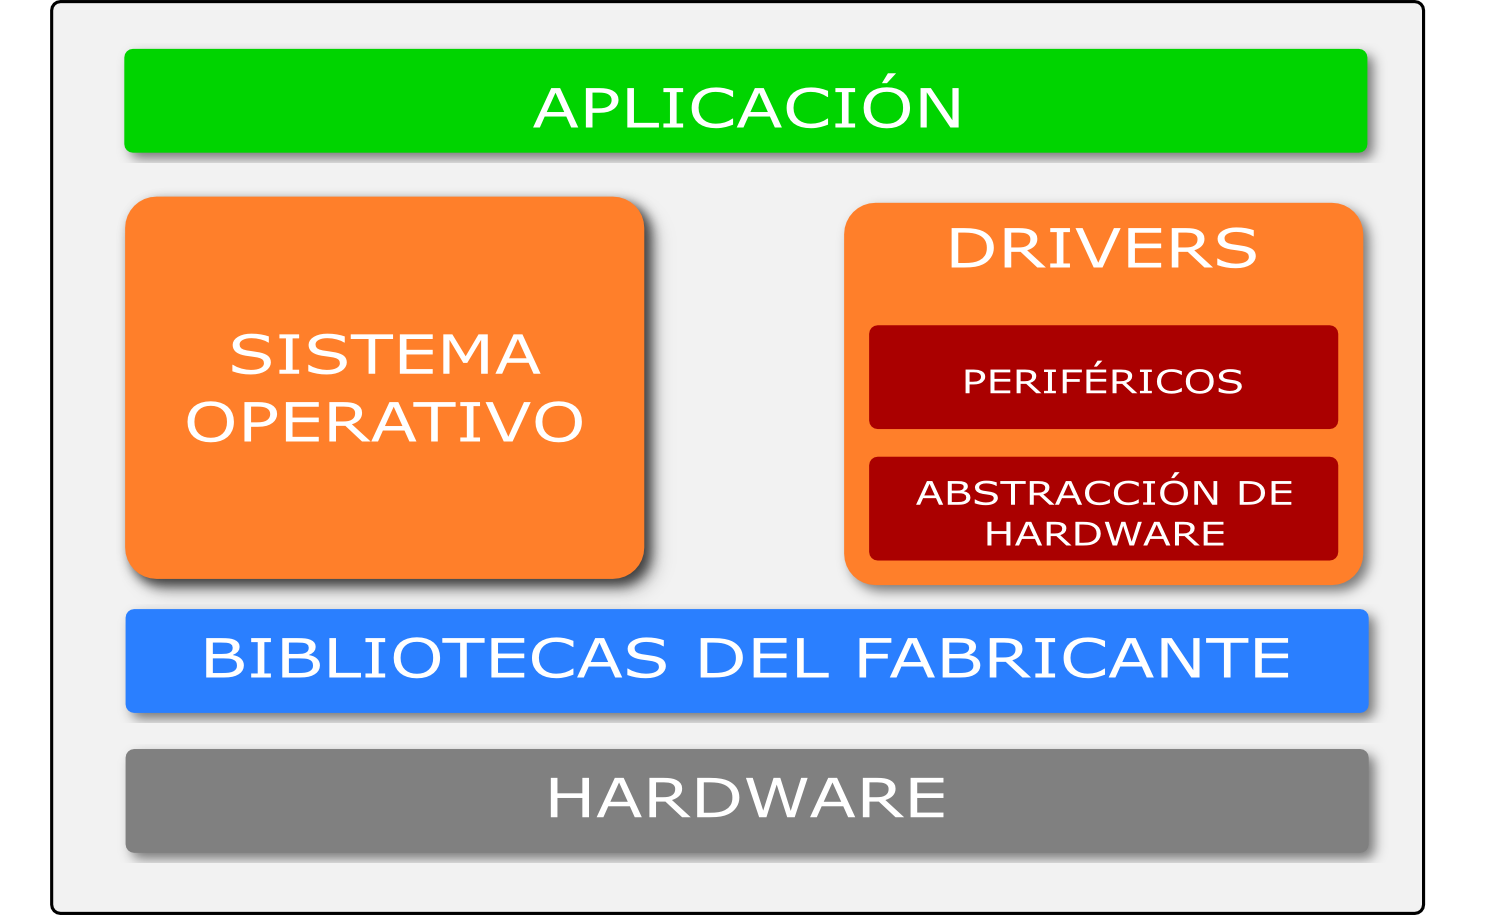
\includegraphics[width=10cm]{./Figures/3_2_2_firmware_diagrama_capas.png}
	\caption{Capas del firmware.}
	\label{fig:firmware_diagrama_capas}
\end{figure}

A continuación se realiza una breve descripción de cada una de las capas:

\begin{itemize}
\item Aplicación. Consiste en el firmware propio del equipo, que utiliza al sistema operativo para implementar la lógica del Smart Plug..
\item Sistema operativo. Consiste en las librerías de FreeOSEK. Como se utilizó un microcontrolador LPC1763 se utilizó la implementación de FreeOSEK para el LPC1769 realizada por Pablo Ridolfi en \citep{repo_ridolfi_freeosek}.
\item Drivers. Dentro de los drivers se encuentras las bibliotecas particulares para controlar tanto los periféricos internos del microcontrolador como los dispositivos externos. La capa de abstracción de hardware, también conocida como HAL (por sus siglas en inglés, Hardware Abstraction Layer), busca generar un nivel más de abstracción entre los drivers de alto nivel y las bibliotecas del fabricante del microcontrolador, lo cual permite, que ante un cambio en el microcontrolador, solamente se deba cambiar la capa HAL.

Para implementar los controladores se utilizó un enfoque orientado a objetos para ordenar las distintas "clases".  Una explicación detallada de este proceso se encuentra en la Subsección \ref{subsec:orientado_a_objetos}.
\item Bibliotecas del fabricante. Son las bibliotecas provistas por NXP para acceder a los periféricos internos del microcontrolador.
\item Hardware. Componentes del Smart Plug.
\end{itemize}

\subsection{Metodología orientada a objetos}
\label{subsec:orientado_a_objetos}

Para implementar los drivers, tanto de los periféricos internos del microcontrolador como de los módulos externos, se decidió implementar una metodología orientada a objetos, a pesar de estar programando en C. La forma de estructurar el código y cada una de las clases surgió a partir de lo explicado por Alex Schreiner en su libro \textit{Object-Oriented Programming With ANSI-C } \citep{schreiner1993}.

Mediante esta forma de programar los drivers se lograron implementar los conceptos de encapsulamiento, polimorfismo y herencia propios de un lenguaje orientado a objetos.

Las clases que se implementaron para este proyecto se pueden ver en el diagrama de clases de la Figura \ref{fig:firmware_diagrama_clases}.

\begin{figure}[h]
	\centering
	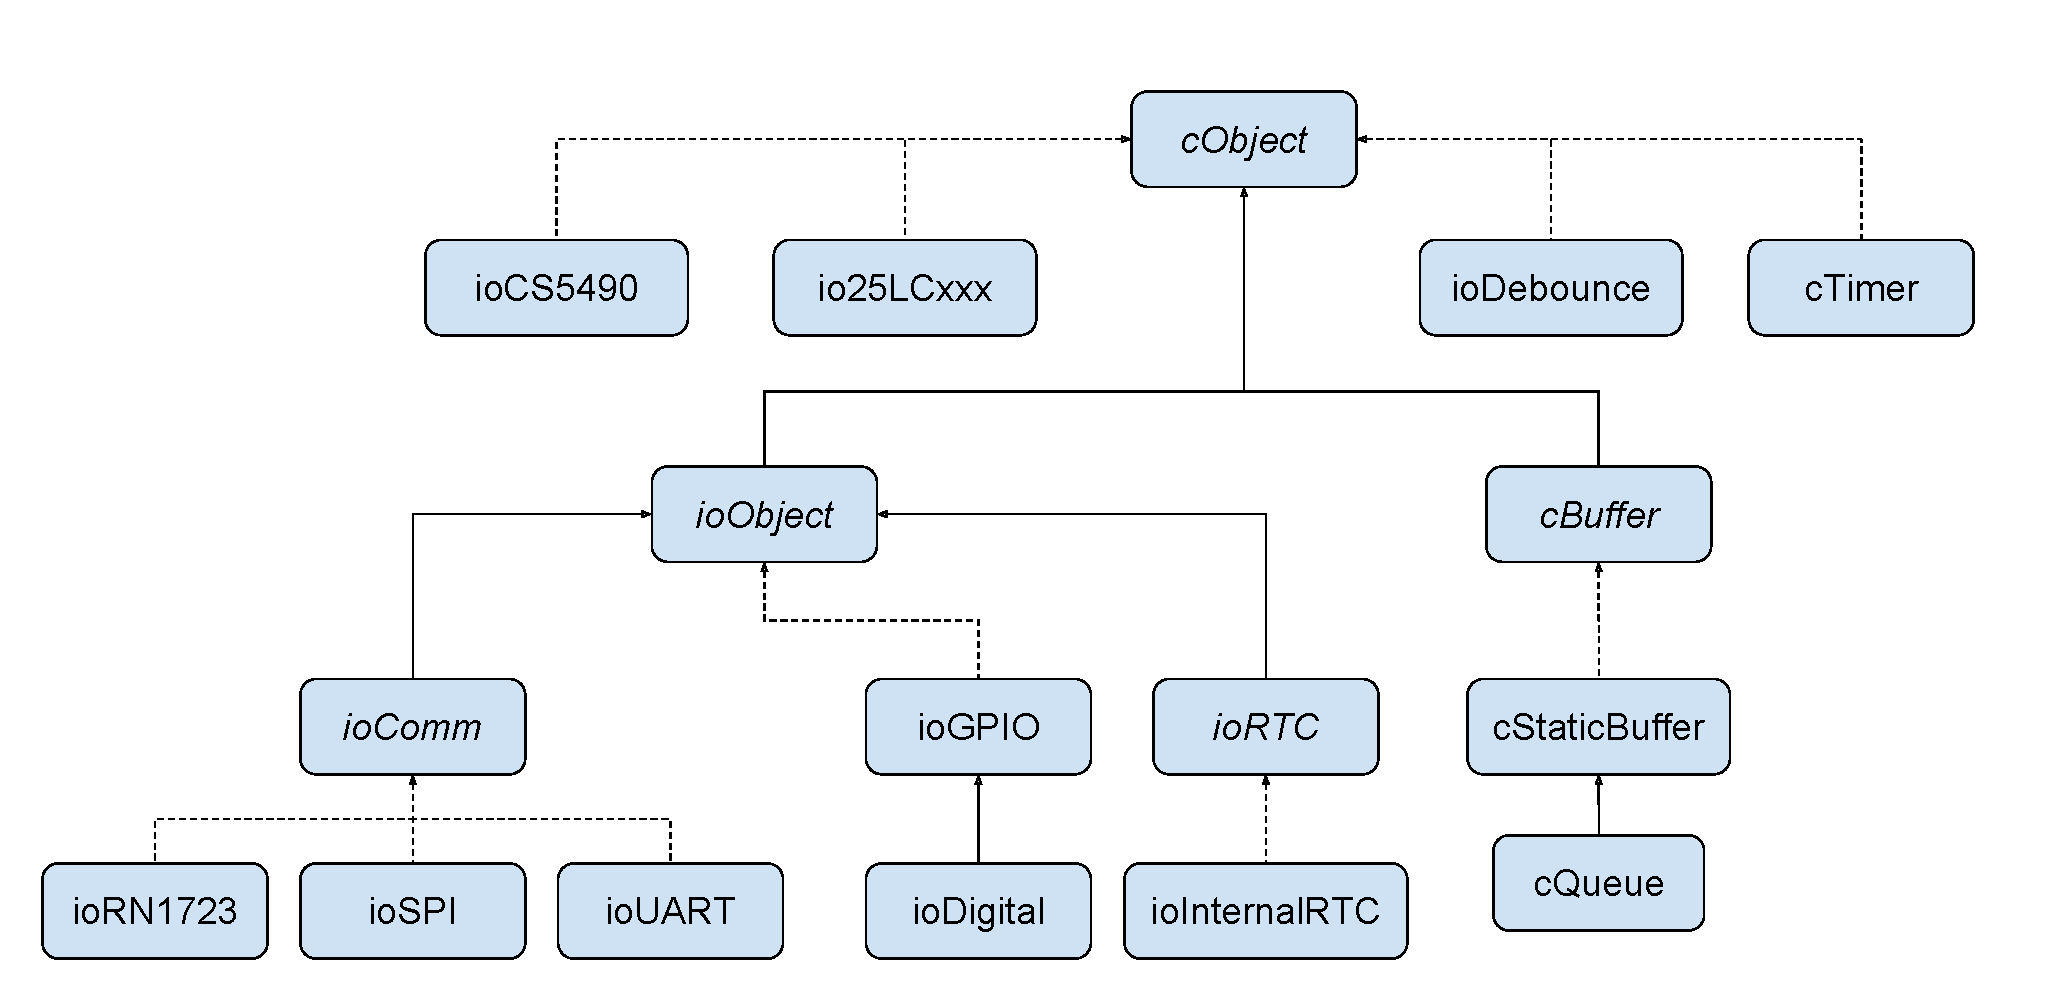
\includegraphics[width=14cm]{./Figures/3_2_3_diagrama-clases-simplificado.pdf}
	\caption{Diagrama de clases de los controladores desarrollados para el firmware.}
	\label{fig:firmware_diagrama_clases}
\end{figure}

La idea general detrás de esta forma para programar módulos de firmware se puede ver en la Figura \ref{fig:firmware_diagrama_interfaces}. Todas las clases implementadas en este trabajo parten de la interfaz \textit{cObject}. Se la llama interfaz y no clase, ya que su comportamiento es similar a las interfaces de Java: \textit{cObject} no implementa la lógica de sus métodos, sino que simplemente declara los prototipos de las funciones (esto se implementa mediante punteros a funciones). Las clases que implementen la interfaz cObject deberán implementar la algoritmia para cada uno de los métodos contenidos en la interfaz \textit{cObject}.

\begin{figure}[h]
	\centering
	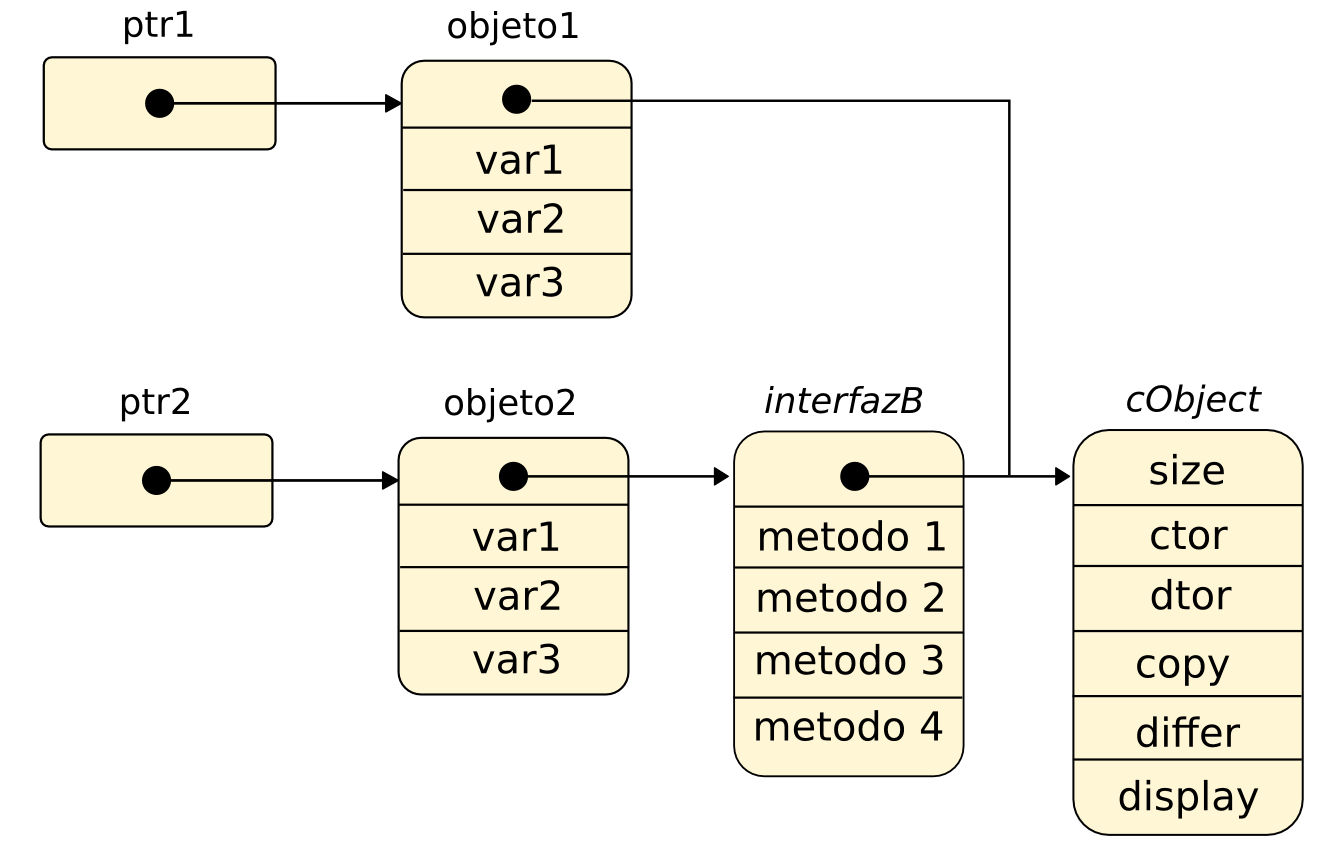
\includegraphics[width=9cm]{./Figures/3_2_3_c_orientado_objetos.png}
	\caption{Creación de interfaces y objetos en C.}
	\label{fig:firmware_diagrama_interfaces}
\end{figure}

Este comportamiento puede verse en la parte superior de la Figura \ref{fig:firmware_diagrama_interfaces}: \textit{objeto1} es una clase que implementa la  interfaz \textit{cObject}. Esta interfaz contiene los métodos básicos necesarios para cualquier otra clase: un constructor, un destructor, una función para crear una copia de un objeto, una función para determinar si dos objetos son iguales y una para mostrar el contenido del objeto de forma comprensible para un humano. Además contiene un campo \textit{size} el cual indica la cantidad de bytes que ocupa una instancia de la clase en memoria RAM.

Por lo tanto \textit{objeto1} debe implementar la lógica de todos los métodos incluidos en \textit{cObject}. Además de implementar la algoritmia, \textit{objeto1} puede contener variables que van a ser propias de cada instancia. En la figura estas serían var1, var2 y var3. Por otro lado, \textit{objeto1} puede declarar funciones que solamente puedan ser utilizadas sobre instancias de la clase \textit{objeto1}.

Finalmente \textit{ptr1} es un puntero a la instancia de \textit{objeto1}. El tipo de variable de \textit{ptr1} es \textit{void*}, es decir que la implementación de la clase queda totalmente encapsulada, ya que la aplicación instancie a \textit{objeto1} no conocerá su estructura interna.

Con esta metodología también es posible implementar la herencia tanto de interfaces como de clases. En la parte inferior de la Figura \ref{fig:firmware_diagrama_interfaces} puede verse un ejemplo de herencia de interfaces. En este caso, la \textit{interfazB} hereda a la interfaz \textit{cObject}, agregando 3 métodos a los ya definidos por \textit{cObject}. Por lo tanto, la clase que implementa la \textit{interfazB} debe implementar todos los métodos, tanto los definidos por \textit{cObject} como los de \textit{interfazB}. En el ejemplo esta clase es \textit{objeto2}, la cual además define 3 variables. Nuevamente \textit{ptr2} es un puntero a \textit{void} el cual apunta al área de memoria donde fue creada la instancia de \textit{objeto2}.

Como puede suponerse esta forma de trabajo requiere además implementar alguna forma de asignación dinámica de memoria. Para este trabajo se decidió implementar un pool de memoria implementado mediante un arreglo de bytes, el cual contiene una sencilla lógica que permite asignar, liberar y unir segmentos continuos (para reducir la fragmentación) del pool de memoria. 

Esta librería es una modificación de la descripta en \citep{an_microchip_malloc}, en la que delante de cada segmento asignado de memoria se coloca un encabezado de dos bytes que indica si está asignado el bloque de memoria o no y la longitud del bloque. El código fuente puede encontrarse dentro de la carpeta \textit{memAlloc} en \citep{repo_firmware}.

Se debe aclarar que esta forma de trabajo no contradice la naturaleza estática del RTOS FreeOSEK. Como condición en la implementación del firmware se estableció que la creación y destrucción de los objetos únicamente se pudiera hacer en el comienzo de la aplicación. De esta forma, cuando el RTOS se encuentra funcionando no se producen más asignaciones dinámicas de memoria y el sistema se comporta como si fuera estático.

En cuanto a las clases desarrolladas se puede mencionar lo siguiente:

\begin{itemize}
\item \textit{ioObject} es una interfaz que hereda a \textit{cObject} y agrega los métodos básicos necesarios para cualquier periférico de entrada/salida: inicialización, habilitación/deshabilitación y escritura/lectura.

\item \textit{ioGPIO} es una clase que implementa a la interfaz \textit{ioObject} y que sirve como base para las clases que describen tipos más específicos de GPIOs, como por ejemplo pines digitales a través de la clase \textit{ioDigital}.

\item \textit{ioDigital} es una clase que herada a \textit{ioGPIO} e implementa la lógica para manejar los GPIO del microcontrolador LPC176x como pines digitales, tanto entradas como salidas.

\item \textit{ioRTC} es una interfaz que hereda a \textit{ioObject} y los métodos básicos necesarios para manejar relojes de tiempo real, tanto internos al microcontrolador, como externos: reset del reloj, lectura y escritura de la hora y fecha.

\item \textit{ioInternalRTC} es una clase que implementa la interfaz \textit{ioRTC} y permite configurar y consultar el RTC interno del microcontrolador LPC176x.

\item \textit{ioComm} es una interfaz que hereda a \textit{ioObject} y agrega los métodos básicos para las clases que modelen periféricos de comunicación: lectura y escritura de cadenas de bytes, determinación de espacio disponible en buffers, habilitación/deshabilitación/consulta de interrupciones.

\item \textit{ioUART} es una clase que implementa la interfaz \textit{ioComm} y que permite manejar las UARTs del microcontrolador LPC176x y las interrupciones relacionadas con estos periféricos. Además agrega el manejo de buffers de recepción y transmisión. La comunicación se puede implementar tanto de forma bloqueante como mediante interrupciones.

\item \textit{ioSPI} es una clase que implementa la interfaz \textit{ioComm} y que permite manejar los SPI del microcontrolador LPC176x. La comunicación es siempre bloqueante.

\item \textit{ioRN1723} es una clase que implementa la interfaz \textit{ioComm} y que permite manejar un módulo WiFi RN1723. Implementa la lógica para poder configurar el módulo, iniciar el modo WPS y AP y manejo de conexiones TCP. Esta clase requiere de otras clases para poder funcionar: \textit{ioUART} para implementar la comunicación con el módulo, \textit{ioDigital} para manejar los pines de reset y algunos GPIO del módulo, \textit{cQueue} para implementar los buffers de recepción y transmisión, \textit{cTimer} para determinar eventos de timeout con el módulo y con las conexiones TCP.

\item \textit{cBuffer} es una interfaz que herada a \textit{cObject} y agrega los métodos necesarios para las clases que modelen contenedores de datos: agregado y borrado de elementos, consulta de elementos, consulta de espacio libre, limpieza del contenedor, etc.

\item \textit{cStaticBuffer} es una clase que implementa la interfaz \textit{cBuffer} y que sirve como base para todas las clases que implementen contenedores de tamaño fijo.

\item \textit{cQueue} es una clase que herera a \textit{cStaticBuffer} e implementa la lógica de una cola, es decir un contenedor de tipo FIFO (First In First Out, primero entra primero sale). Puede contener objetos de cualquier cantidad de bytes pero deben ser todos del mismo tipo.

\item \textit{ioCS5490} es una clase que implementa la interfaz \textit{cObject} que permite manejar el front-end analógico CS5490. Implementa la lógica para poder leer/escribir registros y contiene las variables necesarias para obtener las mediciones eléctricas. Esta clase depende de otras para poder funcionar: \textit{ioUART} para implementar la comunicación con el módulo y \textit{ioDigital} para los pines de reset y de pulsos de energía consumida.

\item \textit{io25LCxxx} es una clase que implementa la interfaz \textit{cObject} que permite manejar memorias EEPROM de la línea 25LC fabricadas por Microchip. Una instancia de esta clase puede ser configurada para escribir/leer/borrar datos de memorias de distintas capacidades, desde 32kbit  hasta 1Mbit. Esta clase depende de \textit{ioSPI} para implementar la comunicación con la memoria externa.

\item \textit{ioDebounce} es una clase que implementa la interfaz \textit{cObject} y permite ejecutar la lógica de un anti-rebote sobre una instancia de la clase \textit{ioDigital}.

\item \textit{ioTimer} es una clase que implementa la interfaz \textit{cObject} y permite implementar timers sencillos y detectar cuando vencen mediante polling. La base de tiempo debe ser establecida por el usuario de la clase \textit{ioTimer}.

\end{itemize}

El código fuente de todas las interfaces y clases puede encontrarse en la carpeta \textit{cObject} en \citep{repo_firmware}. Dentro de esta carpeta también puede encontrarse un diagrama de clases completo (\textit{class\_diag\_cObject.dia}) con los métodos y variables que define cada clase e interfaz.


\subsection{Protocolo de comunicación}
\label{subsection:protocolo}

Para poder intercambiar comandos y respuestas entre la aplicación móvil y los Smart Plugs fue necesario implementar un protocolo de comunicación. Este protocolo está por encima de TCP, el cual se usa para establecer la conexión y proveerla de retransmisiones y corrección de errores. La trama del protocolo desarrollado puede verse en la Figura \ref{fig:formato_trama}. 

\begin{figure}[h]
	\centering
	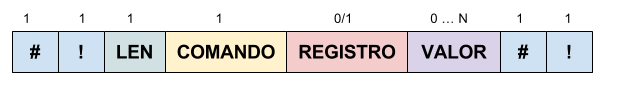
\includegraphics[width=13cm]{./Figures/3_2_4_formato_trama.png}
	\caption{Formato de la trama del protocolo desarrollado para comunicar la aplicación móvil con los Smart Plugs.}
	\label{fig:formato_trama}
\end{figure}

Cada trama va a comenzar y a terminar con los caracteres \textit{\#!}, lo cual facilita la recepción. Además están los siguientes campos:

\begin{itemize}
\item LEN: indica la cantidad de bytes de la trama desde el campo COMANDO hasta los caracteres \textit{\#!} finales.
\item COMANDO: es un byte que indica el código del comando que se está enviando. En la Tabla \ref{tab:comandos_trama} pueden verse todos los posibles comandos.
\item REGISTRO: indica el registro que se quiere leer, escribir o reiniciar. Es un campo opcional, de acuerdo al comando. En la Tabla \ref{tab:registros_trama} puede verse un resumen de los registros disponibles.
\item VALOR: indica el valor que se leyó o se quiere escribir en un registro. Este campo valor va a variar de acuerdo al registro manipulado. En algunos registros, el campo valor son los 4 bytes de un float, en otros registros son los bytes de una cadena de caracteres, etc. Es responsabilidad del receptor interpretar los bytes de este campo de acuerdo al registro.
\end{itemize}



\begin{table}[h]
	\centering
	\caption[Comandos disponibles en el protocolo]{Comandos disponibles en el protocolo.}
	\begin{tabular}{c c p{6cm}}    
		\toprule
		\textbf{Comando} 	 & \textbf{Descipción}  & \textbf{Notas} \\
		\midrule
		0x01  & GET(registro)  				& Pide el valor de un registro \\		
		0x02  & SET(registro, valor)  		& Escribe el valor de un registro \\
		0x10  & NODE\_ON()  					& Enciende la carga manejada por el Smart Plug \\
		0x11  & NODE\_OFF()  				& Apaga la carga manejada por el Smart Plug \\
		0x20  & RESET(registro)  			& Reinicia el valor del registro \\
		0x30  & RESP\_GET(registro, valor)  	& Informa el valor del registro pedido \\
		0x31  & RESP\_SET(registro, valor)  	& Confirma el valor escrito en el registro \\
		0x32  & RESP\_RESET(registro)  		& Confirma que el valor del registro fue reiniciado \\
		0x33  & RESP\_NODE\_ON()  			& Confirma que la carga fue encendida \\
		0x34  & RESP\_NODE\_OFF()  			& Confirma que la carga fue apagada \\
		\bottomrule
		\hline
	\end{tabular}
	\label{tab:comandos_trama}
\end{table}

\begin{table}[h]
	\centering
	\caption[Resumen de los registros disponibles en el protocolo]{Resumen de los registros disponibles en el protocolo.}
	\begin{tabular}{c p{5cm} p{6cm}}    
		\toprule
		\textbf{Comando} 	 & \textbf{Descripción}  & \textbf{Notas} \\
		\midrule
		0x01 a 0x08  	& Registros de mediciones eléctricas  	& Incluye: tensión eficaz, corriente eficaz, factor de potencia, frecuencia, potencia activa, energía total consumida, etc. \\		
		0x10  			& DEVICE\_ID  							& Nombre del dispositivo. Es el nombre que identifica al Smart Plug en la aplicación móvil. \\
		0x15  			& LOAD\_STATE  							& Indica si la carga está encendida o apagada. \\
		0x20 a 022F  	& Registros de programación horaria  	& Es un conjunto de registros que contiene la hora de encendido y la de apagado de la carga para cada día de la semana. \\
		0x30  			& PER\_HOUR\_ENERGY  						& Contiene las 24 mediciones de energía consumida por hora de una determinada fecha. \\
		0x31  			& PER\_HOUR\_ACTIVE\_POWER  				& Contiene las 24 mediciones de potencia activa promedio por hora de una determinada fecha. \\
		\bottomrule
		\hline
	\end{tabular}
	\label{tab:registros_trama}
\end{table}

Una característica a destacar es que este protocolo es de lazo cerrado. Para cualquier comando hay una respuesta que indica que ese comando fue recibido por el Smart Plug. Esta característica es usada por la aplicación móvil, en la cual cuando el usuario cambia un valor de configuración el cambio no se muestra en la pantalla de la aplicación hasta haber recibido la respuesta del comando enviado. De esta forma se asegura que el comando se haya recibido.

La forma en que se implementó el protocolo permite en un futuro agregar nuevos comandos y registros. Solamente será necesario agregar estos nuevos campos en el firmware del Smart Plug y en la aplicación móvil.


\subsection{Uso de los comandos}

A continuación se muestran los distintos escenarios que se pueden dar utilizando el protocolo desarrollado.

En el caso de leer un registro se tiene la secuencia mostrada en la Figura \ref{fig:comunicacion_get}. En este ejemplo, se quiere obtener el valor (campo COMANDO = 0x01 - GET) del registro de la potencia activa (campo REGISTRO = 0x05). Cuando la tareaa taskWiFi en el Smart Plug recibe esta petición le pide el valor actual de la potencia activa a la tarea taskMeter y devuelve el valor con el comando 0x30 (RESP\_GET).

\begin{figure}[h]
	\centering
	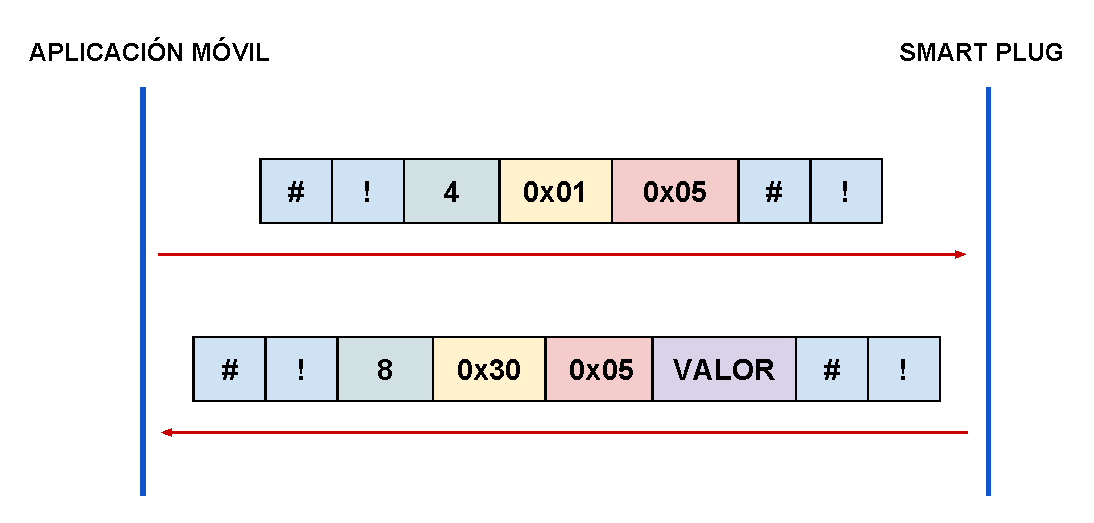
\includegraphics[width=14cm]{./Figures/3_2_5_comunicacion_GET.pdf}
	\caption{Diagrama de comunicación del comando \textit{GET}.}
	\label{fig:comunicacion_get}
\end{figure}

Como se mencionó anteriormente, el campo valor se debe interpretar de distinta forma de acuerdo al registro que se quiera leer. En el caso del registro ACTIVE\_POWER (0x05) el campo valor va a contener los 4 bytes del float de la potencia activa ordenados en formato \textit{Big Endian}.

Cuando se quiere escribir un registro en el Smart Plug, se debe enviar un comando SET y el nuevo valor del registro. En la Figura \ref{fig:comunicacion_set} puede verse la secuencia. En este ejemplo, la aplicación móvil quiere cambiar el registro de la hora de encendido de la carga para los días lunes (REGISTRO = 0x20), con la hora 12:10. 

\begin{figure}[h]
	\centering
	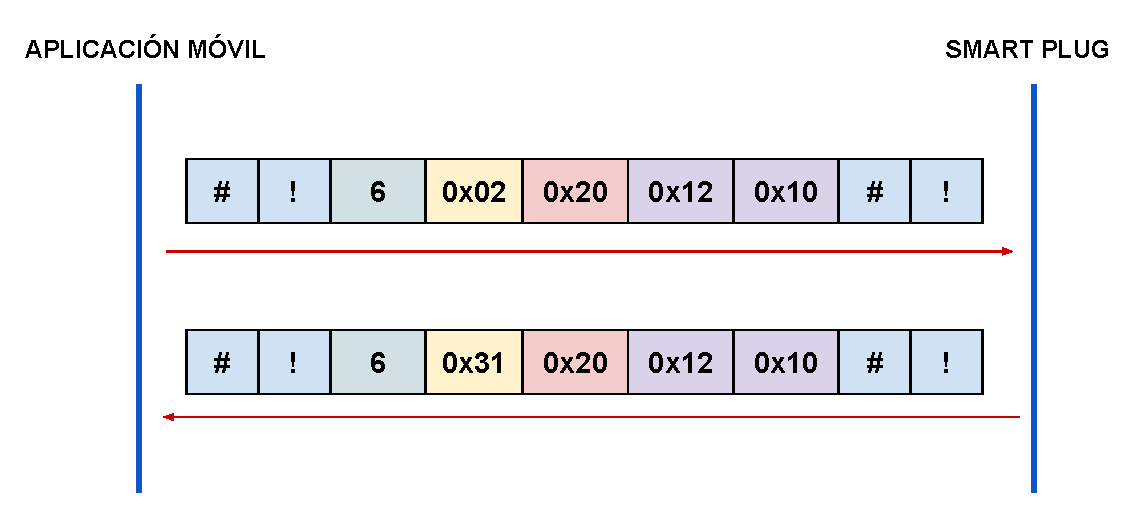
\includegraphics[width=14cm]{./Figures/3_2_5_comunicacion_SET.pdf}
	\caption{Diagrama de comunicación del comando \textit{SET}.}
	\label{fig:comunicacion_set}
\end{figure}

Cuando taskWiFi recibe este comando, escribe el nuevo valor para el registro en la EEPROM, y genera la trama de respuesta con el comando RESP\_SET (0x31) y devuelve el valor que fue cargado en el registro. El hecho de devolver el mismo valor que recibió ayuda a la aplicación móvil a actualizar los datos en sus registros internos.

En este caso se puede ver que el campo valor se debe interpretar como dos bytes, en el cual el primero indica la hora y el segundo los minutos del encendido de la carga.

Además de escribir un valor determinado en un registro, el protocolo permite indicar que se debe reiniciar el valor de un registro. Para lograr esto se debe utilizar el comando RESET (0x20) y el registro que se quiere reiniciar. En el ejemplo de la Figura \ref{fig:comunicacion_reset} se puede ver como se quiere reiniciar el nombre del dispositivo (campo REGISTRO = 0x10).

\begin{figure}[h]
	\centering
	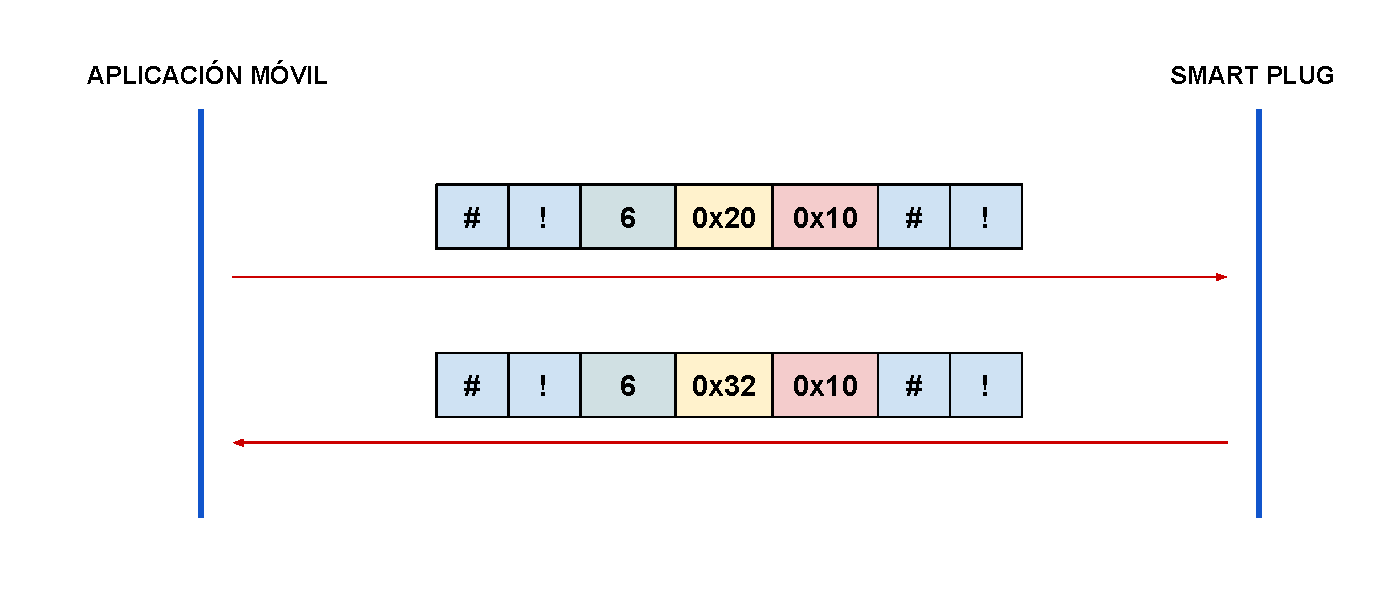
\includegraphics[width=14cm]{./Figures/3_2_5_comunicacion_RESET.pdf}
	\caption{Diagrama de comunicación del comando \textit{RESET}.}
	\label{fig:comunicacion_reset}
\end{figure}

Cuando la tarea taskWiFi recibe este comando va a escribir el valor de fábrica asociado al registro en la EEPROM. Por ejemplo, para el caso del nombre de dispositivo, el valor de fábrica es \textit{Smart Plug}. Sin embargo cada registro tiene un valor de fábrica distinto. Una vez reiniciado el registro, el Smart Plug va a generar una trama de respuesta con el comando RESP\_RESET (0x32) acompañado del registro modificado.

Finalmente existen dos comandos dedicados al control de la carga conectada al Smart Plug. Estos son NODE\_ON (0x10) y NODE\_OFF (0x11). Mediante estos comandos, se le indica al Smart Pug que encienda o apague la carga. En la Figura \ref{fig:comunicacion_node} puede verse la secuencia cuando se envían estos comandos.

\begin{figure}[h]
	\centering
	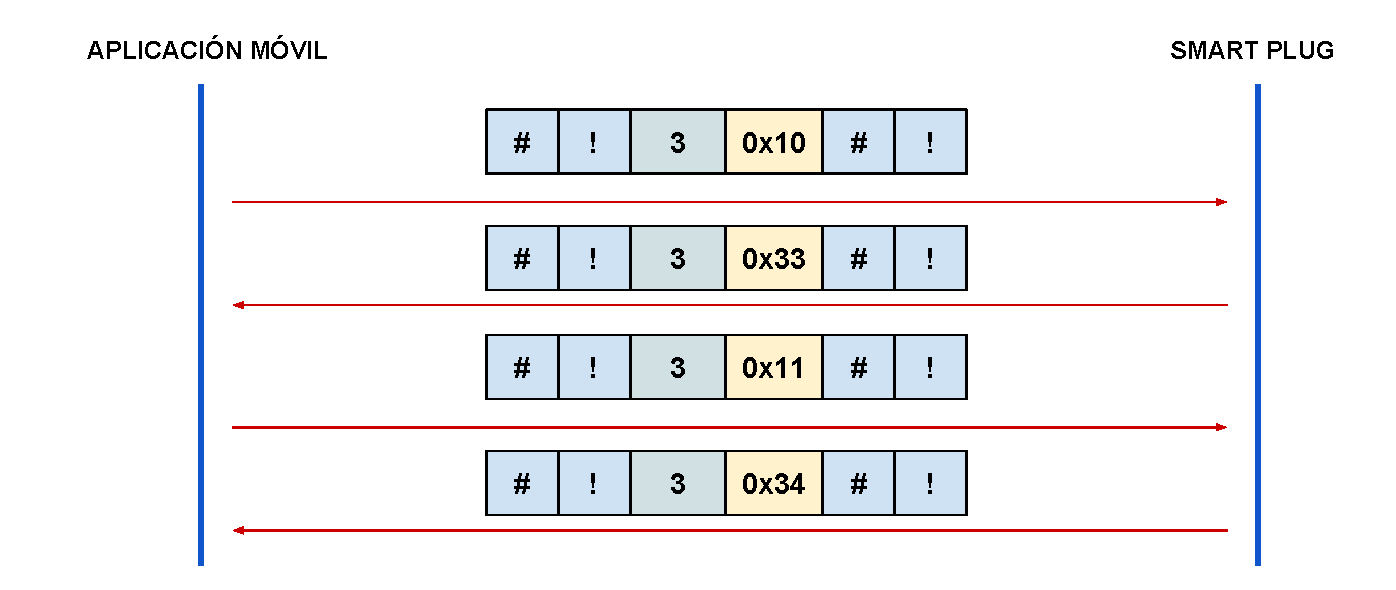
\includegraphics[width=14cm]{./Figures/3_2_5_comunicacion_NODE.pdf}
	\caption{Diagrama de comunicación de los comandos \textit{NODE ON} y \textit{NODE OFF}.}
	\label{fig:comunicacion_node}
\end{figure}

La tarea taskWiFi al recibir estos comandos genera un evento y la tarea taskSmartPlug enciende o apaga la carga a partir del evento recibido. Hecho esto, se devuelve una trama con el comando RESP\_NODE\_ON (0x33) o RESP\_NODE\_OFF (0x34) para que la aplicación móvil tenga la confirmación de que la carga fue conmutada.


\section{Aplicación Android}
\label{section:app}

\subsection{Maqueta de la aplicación}
\label{subsec:app_wireframe}

Antes de comenzar con el diseño de la lógica de la aplicación, fue necesario determinar la forma en la que se iban a presentar los datos al usuario. Para esto se recurrió al uso de una maqueta, en la cual se muestran las pantallas de las que estará compuesta la aplicación y la interacción que hay entre ellas. Cada una de las pantallas presenta el aspecto que realmente debe tener en la aplicación pero no describe la forma en que se debe implementar la lógica de la aplicación.

En la Figura \ref{fig:app_wireframe} puede verse la maqueta completa de la aplicación. La líneas rojas muestran la interacción entre las pantallas y las violetas son comentarios que clarifican el funcionamiento de la pantalla.

\begin{figure}[!h]
	\centering
	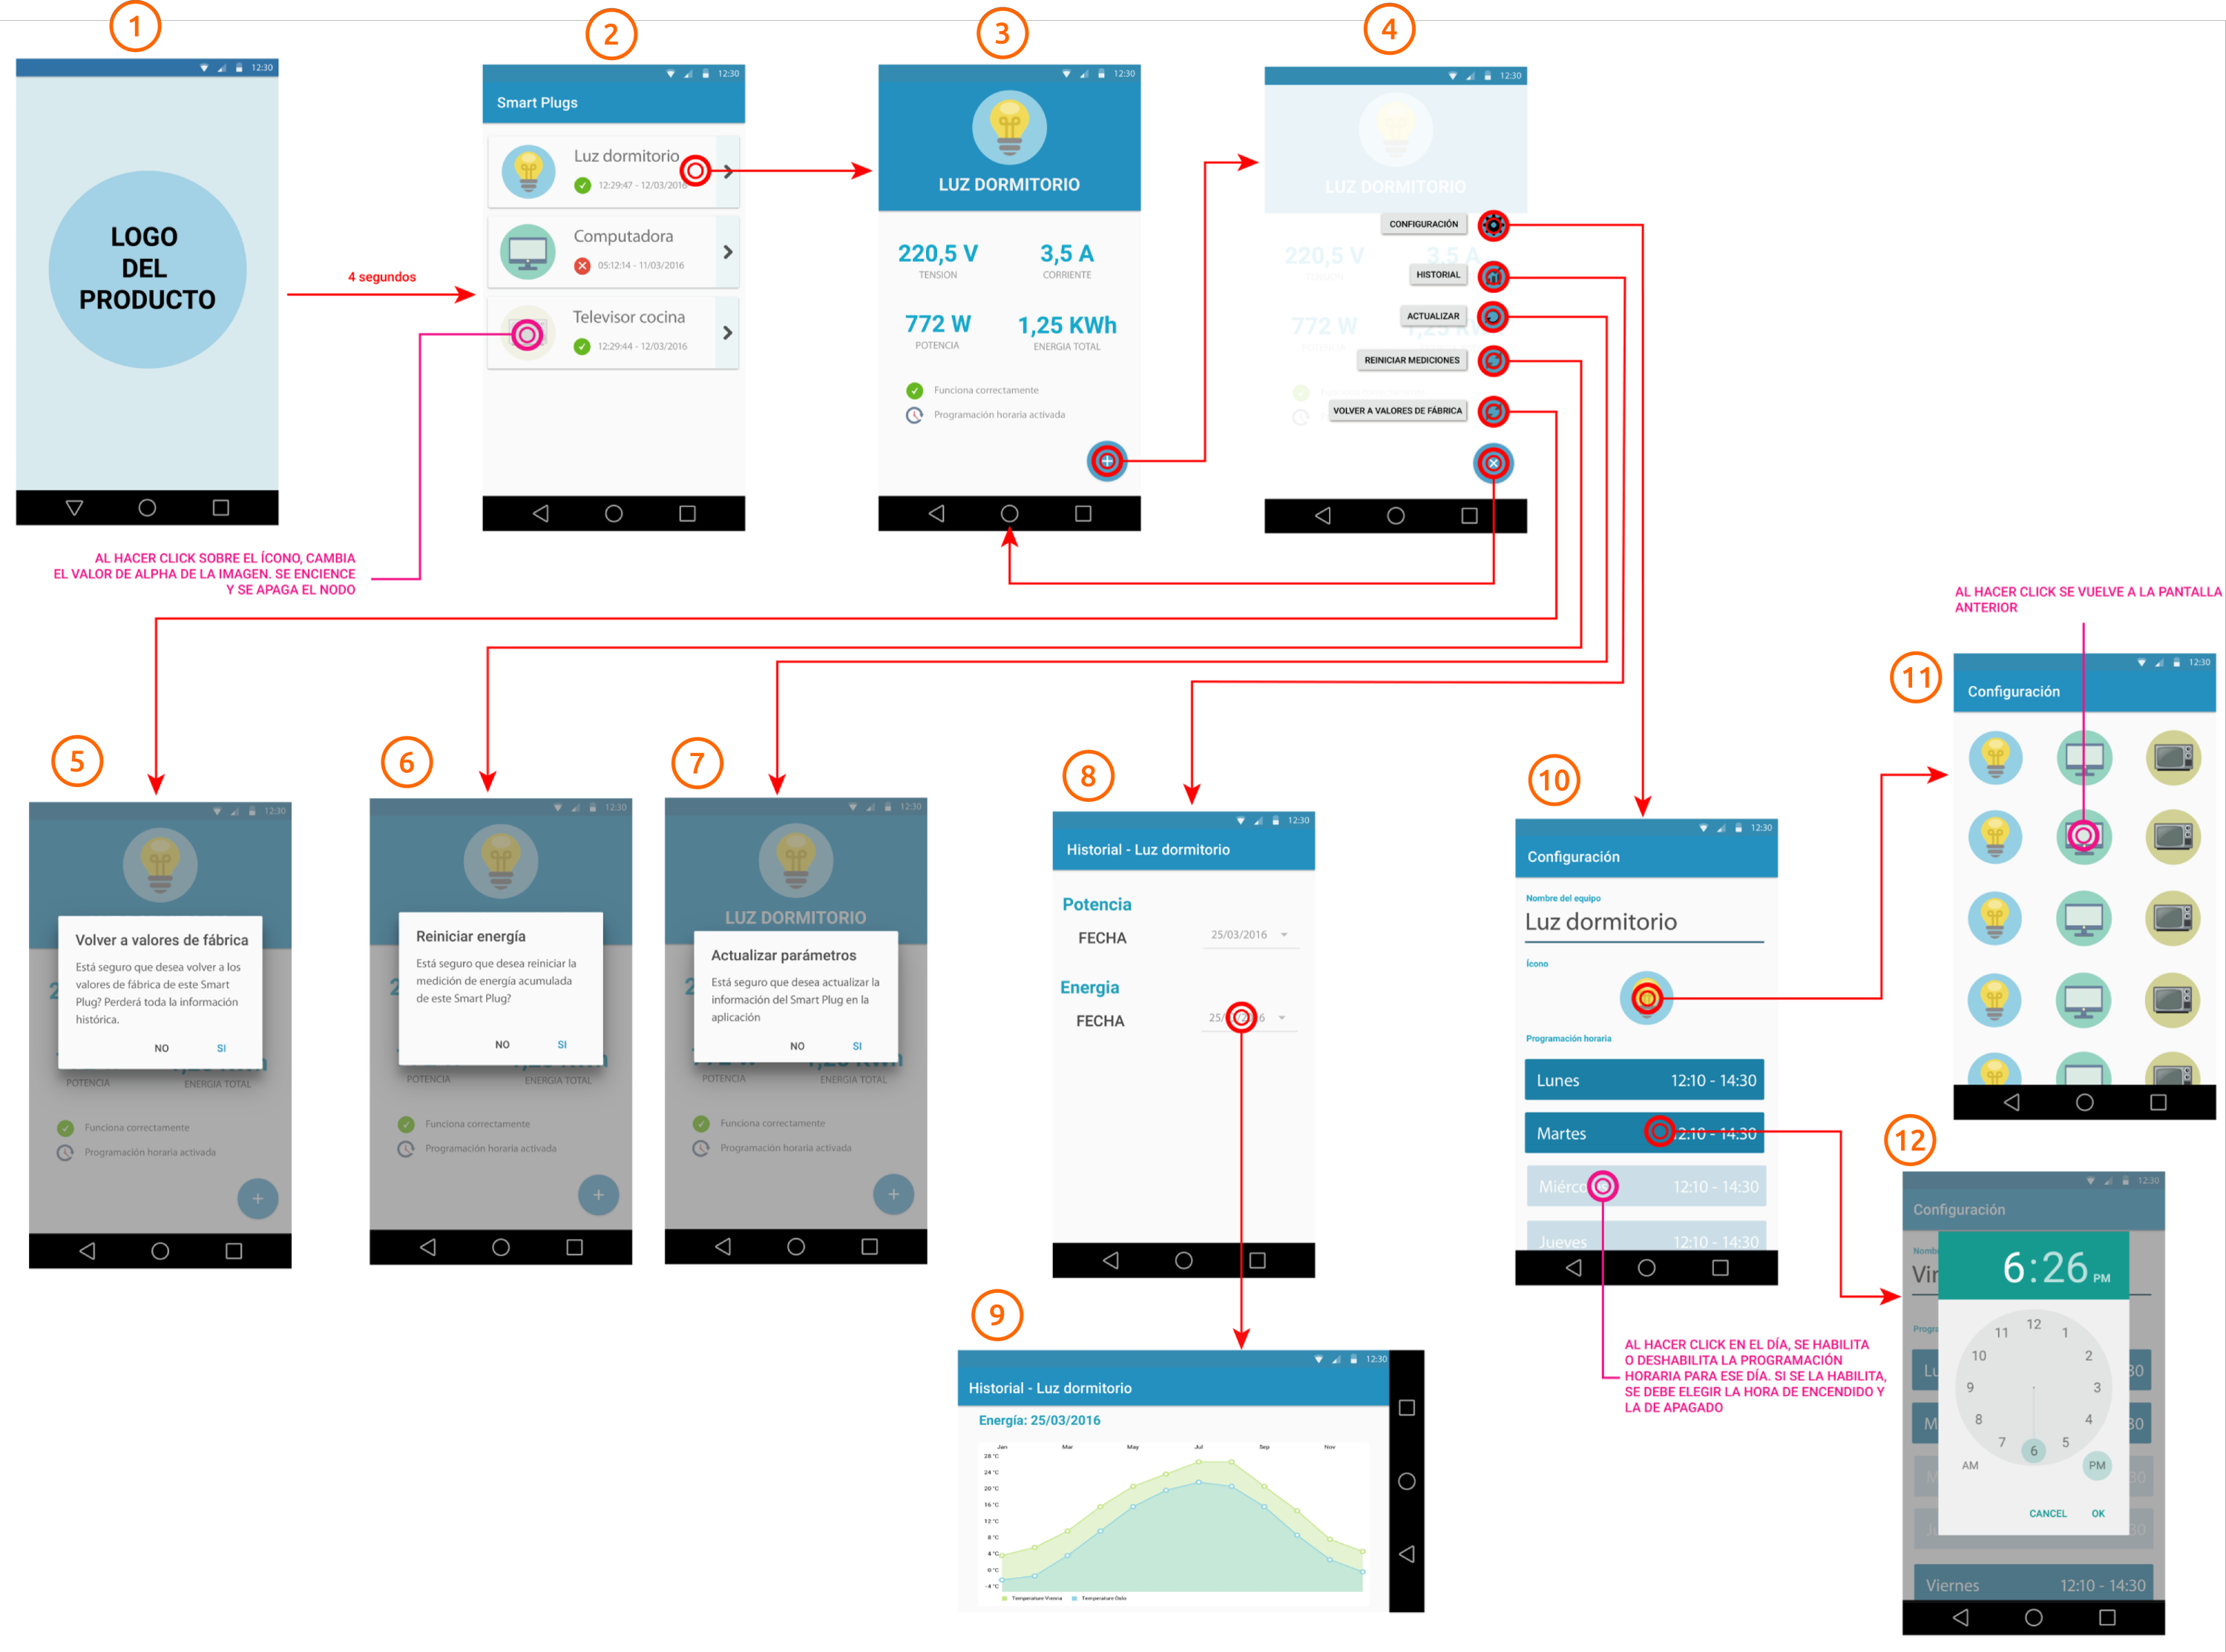
\includegraphics[width=18cm, angle=90]{./Figures/3_3_1_app_wireframe.png}
	\caption{Maqueta de la aplicación móvil.}
	\label{fig:app_wireframe}
\end{figure}

A continuación se describe brevemente el funcionamiento de la aplicación desde el punto de vista del usuario:

\begin{itemize}
\item  Pantalla 1: la aplicación comienza con un \textit{splash screen}, es decir, una pantalla que muestra el logo y el nombre de la aplicación durante unos segundos y luego da paso a la siguiente pantalla.

\item Pantalla 2: luego del \textit{splash screen} se muestra una lista con todos los Smart Plugs que se encontraron en la red WiFi. Como se explicará en la Subsección \ref{subsec:arquitectura_app}, cada Smart Plug se identifica periódicamente dentro de la red WiFi. Estos mensajes periódicos son capturados por la aplicación y en el caso de detectar un Smart Plug que no conocía, lo agregará en la lista. 

Cada uno de los elementos de la lista representa a un Smart Plug. Se va a mostrar el nombre del dispositivo, el estado de la comunicación mediante un tilde verde o una cruz roja y la fecha y hora de la última comunicación exitosa que hubo con ese Smart Plug. Además se muestra un ícono que permite identificar de forma sencilla el dispositivo que realmente está controlando el Smart Plug. 

Pero en la lista, el ícono no cumple únicamente una función pictórica, si se lo presiona se puede conmutar el estado de la carga. Más aún, la opacidad del ícono indica el estado actual de la carga: cuando se lo muestra semi-transparente la carga está apagada y cuando se lo muestra sin transparencia, está encendida.

\item Pantalla 3: cuando en la pantalla 2 se presiona alguno de los Smart Plugs de la lista, la aplicación muestra una vista de detalle del mismo. En esta se volverá a mostrar el ícono asociado al Smart Plug, su nombre, el estado de la comunicación y la fecha y hora de la última comunicación exitosa. Pero además de estos datos se mostrarán las últimas mediciones recibidas desde el equipo. Estas mediciones incluyen: tensión eficaz, corriente eficaz, potencia activa y energía total consumida. Estos datos son actualizados periódicamente, aún cuando la aplicación se encuentra cerrada.

Por otro lado, en esta vista de detalle se encuentra presente, en la esquina inferior derecha de la pantalla, un botón de acción flotante (floating action button) el cual permite acceder a más opciones para gestionar el Smart Plug seleccionado.

\item Pantalla 4: cuando se presiona el botón de acción flotante se despliega un menú el cual incluye la siguiente opciones: Configuración, Historial, Actualizar, Reiniciar mediciones y Volver a valores de fábrica.

\item Pantalla 5: si se presiona la opción de Volver a valores de fábrica, se le preguntará al usuario si confirma que quiere realizar esta acción. En caso afirmativo se le enviará al Smart Plug el comando correspondiente y el cual volverá a sus valores de fábrica, los cuales consisten en:

\begin{itemize}
\item Nombre del dispositivo: Smart Plug.
\item Programación horaria de encendido/apagado deshabilitada.
\item Se reinicia el registro la energía consumida.
\item Se eliminan las mediciones históricas de potencia activa y enrgía consumida por hora, tanto en el Smart Plug como en la aplicación.
\end{itemize}

\item Pantalla 6: si se presiona la opción Reiniciar mediciones, se le preguntará al usuario si confirma que quiere realizar la acción. En caso afirmativo, se enviarán los comandos correspondientes al Smart Plug. Cuando se realiza esta acción se reiniciará el registro de la energía consumida y se eliminarán las mediciones históricas de potencia activa y energía consumida por hora. 

Se decidió incorporar esta opción para ayudar en los casos en los que, por ejemplo, se cambia la carga que está controlando el Smart Plug, por lo que se desea eliminar los registros de la anterior carga ya que podrían llevar a confusiones en la interpretación de los datos.

\item Pantalla 7: cuando se presiona la opción Actualizar, una caja de diálogo le preguntará al usuario si confirma la acción. En caso afirmativo, se forzará el proceso de actualización de los datos del Smart Plug, es decir, se le pedirán las últimas mediciones, sus parámetros de configuración y sus mediciones históricas para actualizar la información en la aplicación. Este comando es útil cuando se necesita conocer la información actual por ejemplo, de una medición y no se puede esperar hasta la próxima consulta periódica que realiza la aplicación.

\item Pantalla 8: al presionar la opción Historial se accede a todas las mediciones históricas que se recibieron desde el Smart Plug. Estas mediciones históricas consisten en las mediciones que realizó en cada hora del día, tanto de la potencia activa promedio como de la energía consumida. En esta pantalla se podrá elegir el día que se quiere ver y el parámetro que se desea consultar mediante dos listas de fechas. Se debe aclarar que aunque el Smart Plug retenga las mediciones de los últimos 7 días, la aplicación puede retener hasta 20 días.

\item Pantalla 9: cuando se elije una fecha la pantalla gira para mejorar la visualización de los datos en forma de gŕafico. En este gráfico se va a representar la potencia activa por hora (en Watt) vs la hora del día o la energía consumida por hora (en kWh) vs la hora del día. Se puede realizar zoom y desplazarse por el gráfico arrastrando el dedo.

Estos gráficos representan una de las características distintivas de este producto, ya que permite visualizar de forma sencilla mediciones que pueden ser aprovechadas para conocer el consumo de un determinado aparato eléctrico.

\item Pantalla 10: contiene los parámetros configurables del Smart Plug seleccionado. Se accede a esta pantalla presionando la opción Configuración en el menú del botón de acción flotante. Los parámetros que se pueden configurar son básicamente tres: el nombre del dispositivo, el ícono del Smart Plug y la programación horaria para cada día de la semana.

En cuanto al nombre del dispositivo, se puede configurar un nombre de hasta 32 caracteres. Una vez ingresado se debe presionar la flecha que se encuentra a la derecha del control para ingresar el texto. Este nombre quedará configurado en el Smart Plug, por lo que todas las aplicaciones que tengan registrado a este Plug, verán el nuevo nombre.

Al presionar el ícono del Smart Plug se mostrará la pantalla 11, permitiendo elegir de una lista de íconos. Una vez que se selecciona uno de estos se vuelve a la pantalla 10. El ícono es una información propia de la aplicación móvil y no queda guardado en el Smart Plug. por lo tanto distintas aplicaciones móviles pueden asignar íconos diferentes a un mismo Plug.

Finalmente, la programación horaria puede ser habilitada y deshabilitada para cada día de la semana individualmente. La transparencia del recuadro que contiene la información de cada día indica si la programación horaria está habilitada: si el recuadro es semi-transparente, está deshabilitada, pero si no es transparente, está habilitada. 

Si se presiona cualquiera de los días se mostrará la pantalla 12 invitando a ingresar la hora de encendido de la carga. Se puede elegir cambiar esta hora o dejar la que estaba ya configurada. Una vez configurada la hora de encendido se volverá a mostrar la pantalla 12 para ingresar la hora de apagado; se procede de igual forma que antes. Cuando se ingresan ambas horas se configura el Smart Plug con estos nuevos valores.

Si en cambio de desea deshabilitar esta opción para un día de la semana, se debe mantener presionado el recuadro del día elegido. Cuando se deshabilite la opción, el recuadro se mostrará semi-transparente.

\end{itemize}


\subsection{Arquitectura de la aplicación}
\label{subsec:arquitectura_app}

La estructura general de la aplicación móvil puede verse en la Figura \ref{fig:app_arquitectura}. A continuación se describirán los elementos principales que la componen y la interacción entre ellos.

\begin{figure}[h]
	\centering
	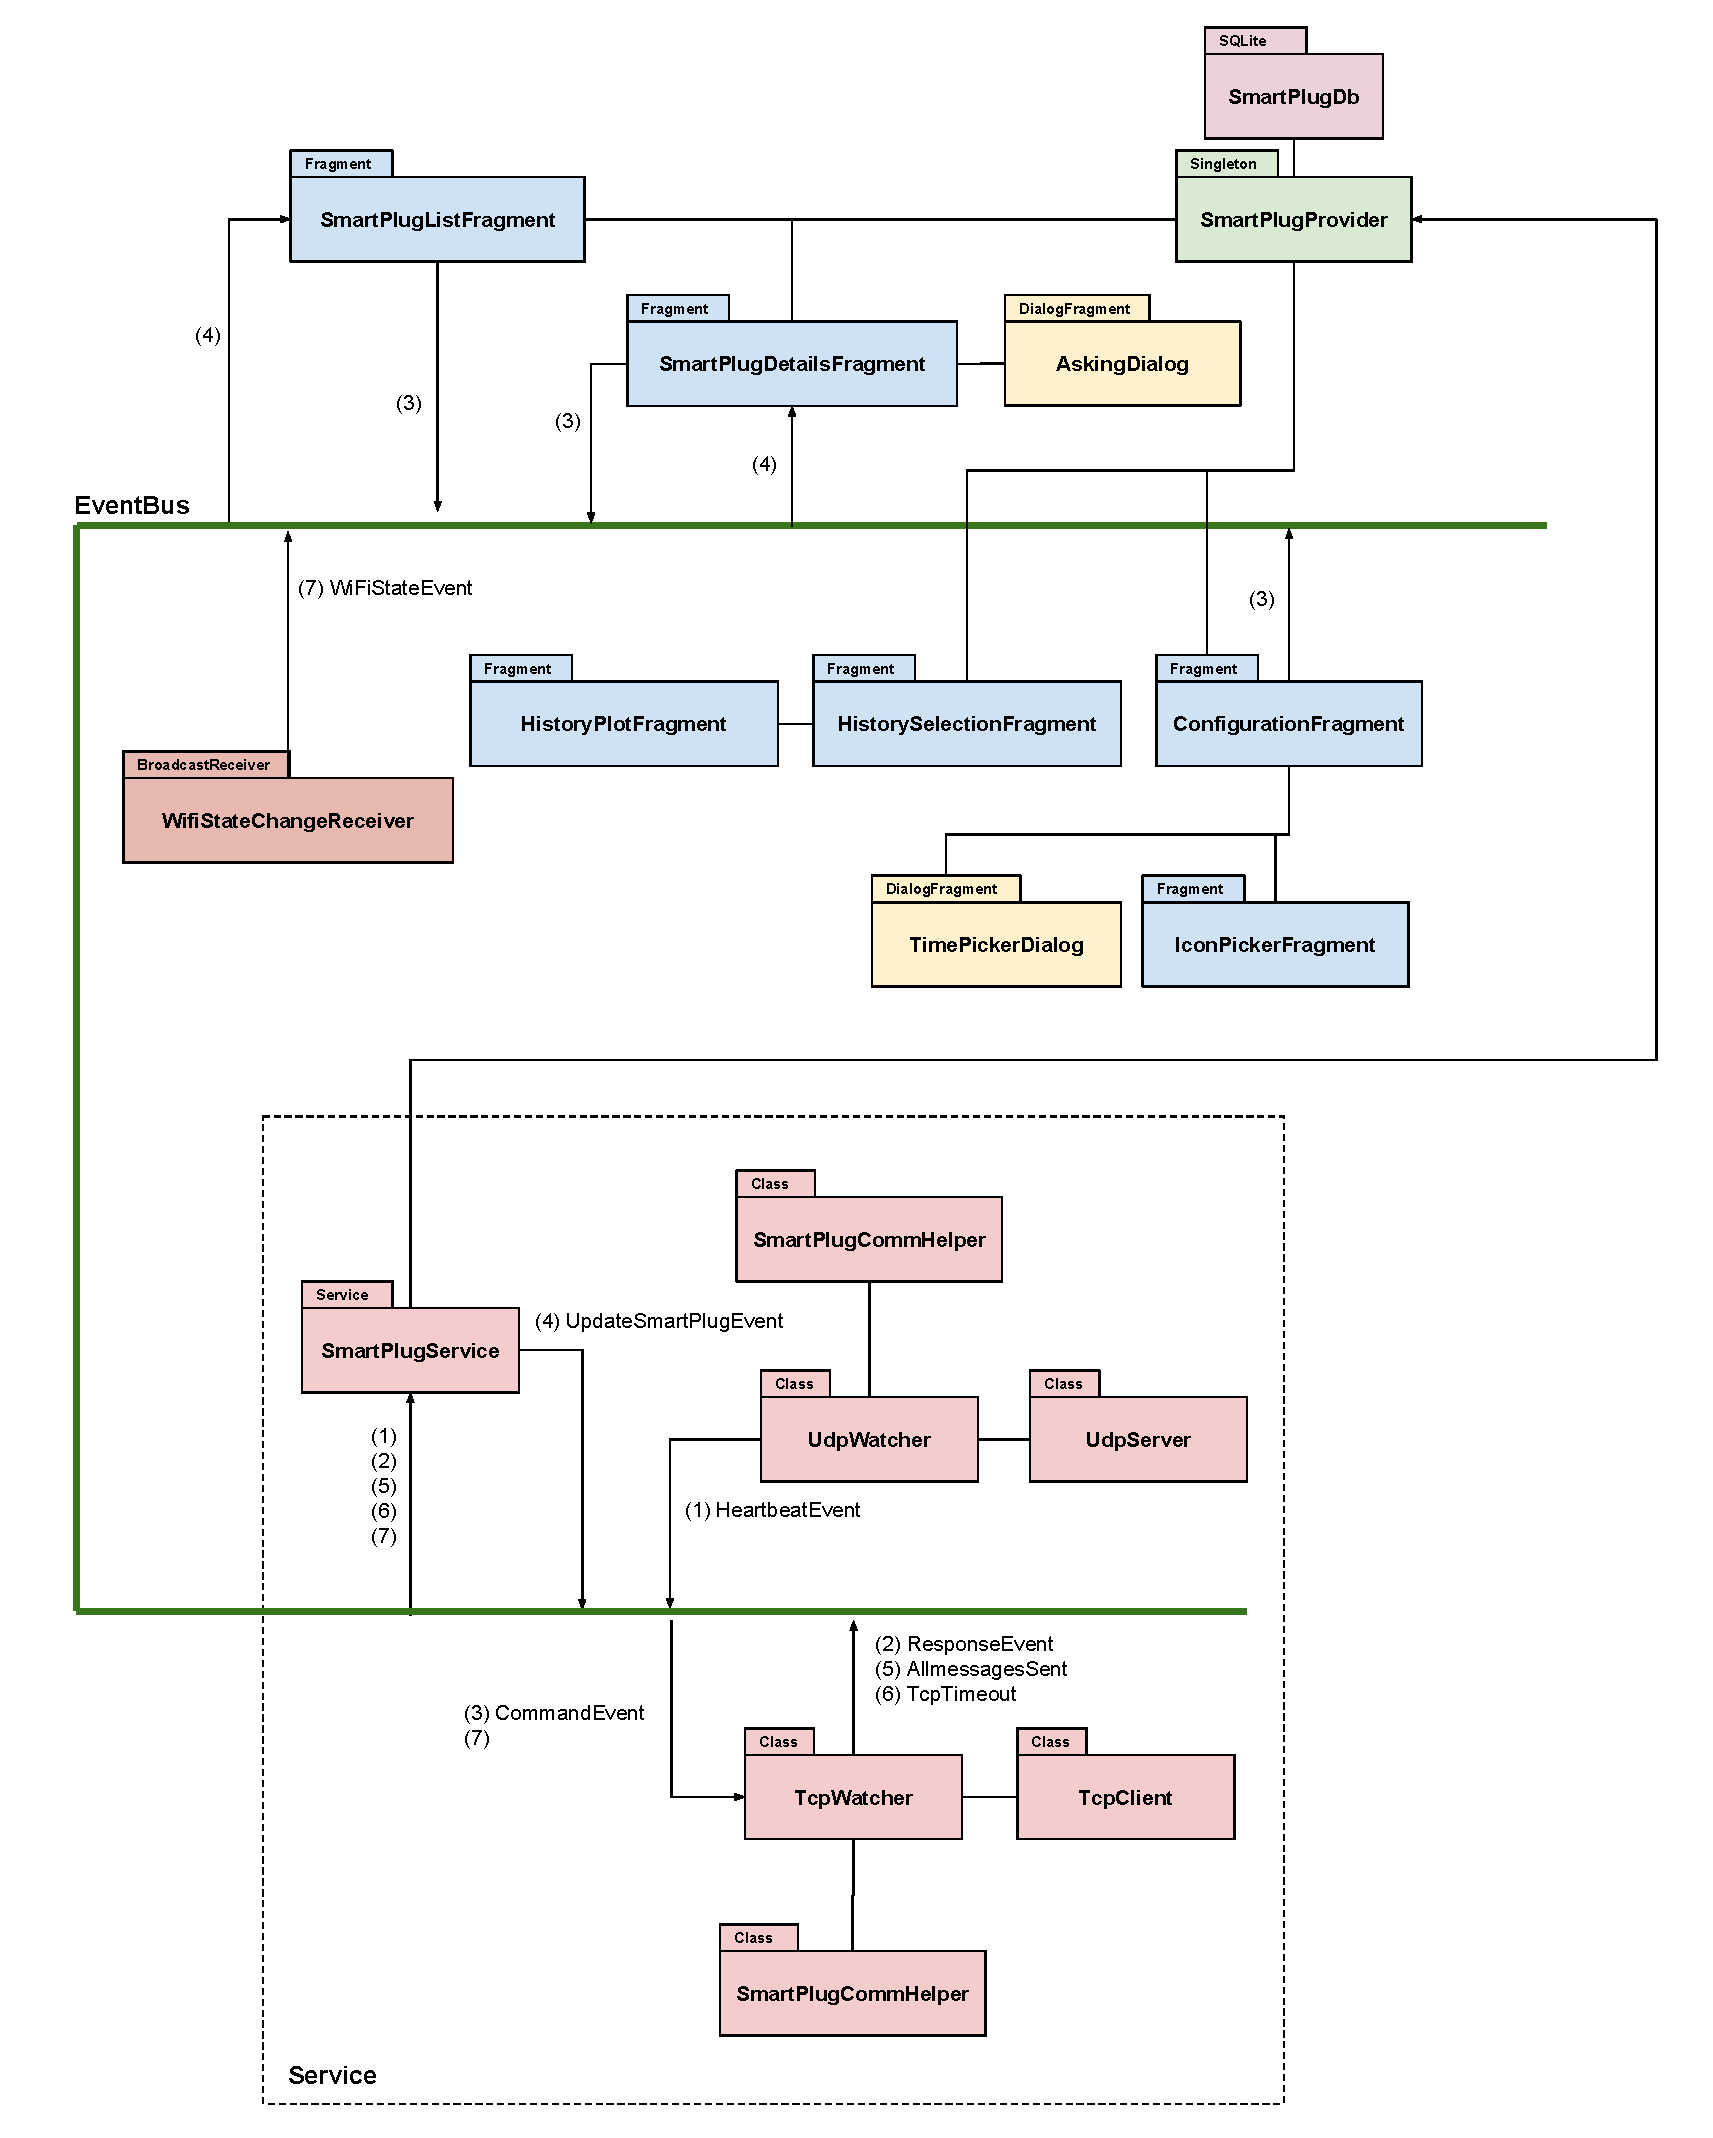
\includegraphics[width=15cm]{./Figures/3_3_2_app-arquitectura.pdf}
	\caption{Relación entre las clases desarrolladas para la aplicación móvil.}
	\label{fig:app_arquitectura}
\end{figure}

\begin{itemize}
\item EventBus. La forma que se eligió para comunicar todos los elementos de la aplicación es un bus de eventos. Para esto se utilizó unalibrería llamada EventBus, desarrollada por la empresa Green Robot \citep{eventbus_web}. Esta librería consiste en un esquema de suscripción a un bus en el que cualquier clase puede publicar un evento, el cual va a ser recibido por todas las clases que se hayan suscrito al mismo. Además esta librería se encarga de la comunicación entre clases que se encuentran en distintos threads.

Los eventos no son más que objetos de java que contienen información de interés para la clase que los recibe. En el caso concreto de la aplicación, se crearon varios eventos, los cuales pueden verse en la Figura \ref{fig:app_arquitectura} representados mediante un número al lado de las flechas que unen las clases al bus de eventos común. Estos eventos son:


\begin{enumerate}
\item HeartbeatEven: este evento se genera cada vez que el servidor UDP recibe un mensaje periódico de uno de los Smart Plugs. Con este mensaje se logra mantener actualizada la información del Smart Plug, especialmente la IP que le fue asignada por el DHCP dentro de la red WiFi.
\item ResponseEvent: contiene la respuesta recibida por el cliente TCP de la aplicación a un comando enviado a un Smart Plug.
\item CommandEvent: contiene los elementos de una trama que se tiene que enviar a un determinado Smart Plug. Cualquier componente de la aplicación que quiera enviar un mensaje a un Smart Plug debe enviar una instancia de este evento al EventBus.
\item UpdateSmartPlugEvent: este evento se genera cada vez que se recibe nueva información de un Smart Plug. De esta forma, los fragmentos que están suscritos a este evento actualizan la información mostrada si el Smart Plug que se actualizó coincide con el que se está mostrando. 

Por ejemplo cuando se enciende la carga de un Smart Plug desde la lista de Plugs, este evento permite que la transparencia del ícono del Plug cambie al recibir la confirmación de que la carga fue encendida. Si no estuviera este evento el ícono se actualizaría cuando se regenerara la vista del fragmento.
\item AllmessagesSent: se genera cuando el cliente TCP de la aplicación no tiene más mensajes que enviar en la lista de mensajes pendientes. Se utiliza para que la aplicación libere ciertos recursos que retiene mientras se están enviando los mensajes.
\item TcpTimeout: se genera cuando se produce un timeout esperando la respuesta a un comando, o cuando se produce otro error en la comunicación. Cada uno de estos errores y timeouts se van sumando en un contador asociado a cada Smart Plug y cuando se superan los 5 eventos, se indica que existe un problema en la comunicación con el Plug.
\item WiFiStateEvent: se genera cada vez que cambia el estado de la conexión del teléfono a la red WiFi. Esto le sirve a la aplicación para conocer si está conectado a la red WiFi o no. En caso de no estarlo, no se intentan enviar mensajes a los Plugs ya que no se los va a poder alcanzar.
\end{enumerate}

\item Servicio. Cuando se inicia la aplicación por primera vez inicia una instancia de la clase SmartPlugService que hereda a la clase Service de Android. Un servicio permite implementar una parte de la lógica que se debe ejecutar por un tiempo prolongado de tiempo en un thread distinto del thread principal de la aplicación. Además, como fue configurado en el caso de esta aplicación, este servicio se mantiene ejecutándose aún cuando la aplicación se encuentra cerrada.

Dentro del servicio se implementa la lógica para la consulta periódica de los Smart Plugs que identificó la aplicación. Cada 10 minutos, el servicio se ejecutará y realizará una serie de consultas a todos los Smart Plugs que conozca, preguntando el últimos valor de las mediciones, algunos parámetros de configuración para ver si fueron cambiados por otra aplicción y el estado de la carga, para ver si fue conmutada por otra aplicación.

Además, cada 1 hora aproximadamente, el servicio le pedirá a todos los Smart Plugs las mediciones históricas del día para conocer los valores de potencia activa y energía consumida por hora de la última hora.

Toda la información que es recibida desde los Smart Plugs es volcada a una base de datos propia de la aplicación (smartPlug.db) la cual va a ser consultada por todos los otros elementos de la aplicación cuando necesiten conocer la última información de un Smart Plug. El acceso a la base de datos se realiza a través de la clase llama SmartPlugProvider.

La ejecución periódica de este servicio se logra configurando una alarma mediante el AlarmManager de Android que se ejecute cada 10 minutos. A las 6 veces que se ejecute esta alarma se considerará que pasó una hora y se harán las consultas correspondientes a los Plugs.


\item TcpWatcher y TcpClient. Estas clases se ocupan de establecer la comunicación TCP con los distintos Smart Plugs. La clase TcpWatcher se suscribe a los eventos de tipo CommandEvent y cada vez que recibe uno lo coloca dentro de una lista, la cual va leyendo para determinar las tramas que debe enviar. La comunicación propiamente dicha está implementada en la clase TcpClient, la cual gestiona la conexión y los posibles errores que se pueden producir. 

Para armar las tramas de acuerdo a lo establecido por el protocolo desarrollado en este trabajo, la clase TcpWatcher utiliza los métodos de la clase SmartPlugCommHelper que se encarga de encapsular los formatos de las tramas de acuerdo al comando y registro que se está manipulando.

Si se recibe una respuesta del Smart Plug, la clase TcpWatcher generará un evento del tipo ResponseEvent. En caso de que se produzca un error, generará un evento del tipo TcpTimeout. Cuando termine de enviar todos los mensajes que tenía pendiente generará el mensaje AllmessagesSent.

\item UdpWatcher y UdpServer. Este par de clases se ocupa de escuchar los mensajes periódicos que son enviados a la dirección de broadcast de la red por parte de los Smart Plugs. Los mensajes periódicos son enviados al puerto UDP 55555. Cada vez que UdpServer (que es la clase que implementa concretamente el servidor UDP) recibe un nuevo datagrama UDP, se lo comunica a la clase UdpWatcher.

La clase UdpWatcher parsea el datagrama con la ayuda de la clase SmartPlugCommHelper y determina de qué Smart Plug provino. Con esta información genera un evento del tipo HeartbeatEvent. Dentro del datagrama UDP se encuentra el ID único que identifica a cada Smart Plug, el cual se va a tulizar dentro de la aplicación para identificar unívocamente a un Plug.

\item SmartPlugProvider. Es la clase encargada de acceder a la base de datos de la aplicación (smartPlug.db) en donde está contenida la información de los Smart Plugs encontrados. Esta base de datos está compuesta por 4 tablas, las cuales pueden verse en la Figura \ref{fig:app_sqlite}. A continuación se da una breve descripción de cada tabla:

\begin{itemize}
\item StaticInfo. Continene la información básica del Smart Plug, como es su nombre y el ícono que tiene asociado. Todas las entradas de las tablas van a estar asociadas al número de ID único del Smart Plug el cual es recibido en cada mensaje UDP que envía el Plug.
\item OnOffTimes. Contiene los horarios de encendido y apagado para cada día de la semana así como también una variable que indica qué días están habilitados.
\item Measurements. Contiene las mediciones históricas recibidas desde cada Smart Plug. En cada entrada de la tabla se guarda la fecha a la que corresponden las mediciones y las 24 mediciones de ese día, al igual que el tipo de medición (potencia activa o energía consumida).
\item InstantaneousInfo. Contiene información variable de cada Smart Plug. Es información incluye: la última IP en la que se encontró al Smart Plug, la última fecha y hora de comunicación, el estado de la carga, las últimas mediciones instantáneas, la cantidad de timeouts que se produjeron en la comunicación y el estado de la comunicación.
\end{itemize}

Toda clase que desee acceder a la base de datos, debe hacerlo a través de la clase SmartPlugProvider ya que implementa toda la lógica relacionada con la manipulación de la base de datos.

\item WiFiStateChangeReceiver. Es una clase que extiende a BroadcastReceiver y se encarga de recibir los intents de Android relacionados con los cambios en la conectividad. De esta forma determina si el teléfono se encuentra conectado a la red WiFi o no. En caso de no estar conectado los mensajes a los Smart Plugs no se envían.

\end{itemize}


\begin{figure}[h]
	\centering
	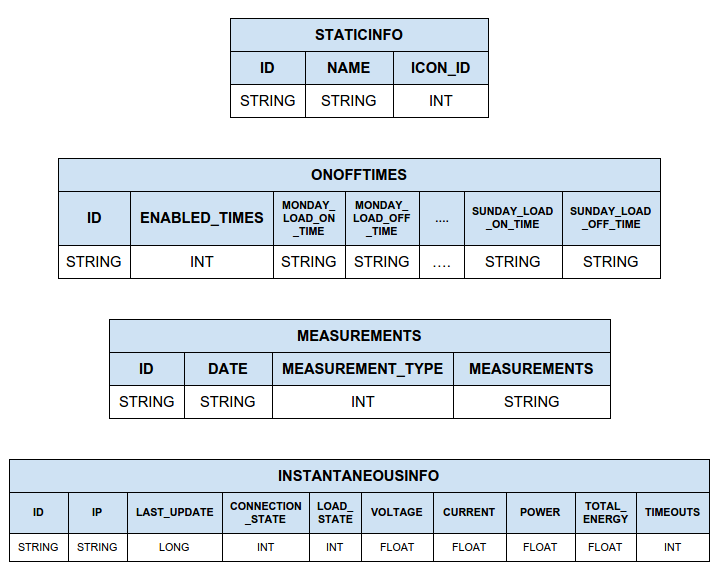
\includegraphics[width=13cm]{./Figures/3_3_2_tablas_sqlite.png}
	\caption{Tablas que componen la base de datos de la aplicación.}
	\label{fig:app_sqlite}
\end{figure}

La lógica asociada a cada una de las pantallas mostradas en la maqueta en la Subsección \ref{subsec:app_wireframe} se implementaron mediante fragments, para flexibilizar el diseño de la interfaz gráfica. La relación entre las pantallas de la Figura \ref{fig:app_wireframe} y los nombres de los fragmentos es la siguiente:

\begin{enumerate}
\item Pantalla 1: SplashScreenFragment.
\item Pantalla 2: SmartPlugListFragment.
\item Pantalla 3: SmartPlugDetailsFragment.
\item Pantalla 4: SmartPlugDetailsFragment.
\item Pantalla 5: AskingDialog.
\item Pantalla 6: AskingDialog.
\item Pantalla 7: AskingDialog.
\item Pantalla 8: HistorySelectionFragment.
\item Pantalla 9: HistoryPlotFragment.
\item Pantalla 10: ConfigurationFragment.
\item Pantalla 11: IconPickerFragment.
\item Pantalla 12: TimePickerDialog.
\end{enumerate}

La lógica de alto nivel que implementa cada fragment fue explicada en la Subsección \ref{subsec:app_wireframe}. El código fuente de la aplicación puede encontrarse en \citep{repo_app}.


% Chapter Template

\chapter{Ensayos y Resultados} % Main chapter title

\label{Chapter4} % Change X to a consecutive number; for referencing this chapter elsewhere, use \ref{ChapterX}

%----------------------------------------------------------------------------------------

La idea de este capítulo consiste en describir las pruebas realizadas sobre el producto y explicar los resultados obtenidos.

\section{Ensayos de caja negra}

Luego de realizar la implementación de cada uno de los aspectos del producto, hardware, firmware y aplicación móvil, se procedió a validar los requerimientos establecidos durante la planificación. Para esto se escribió una serie de pruebas que buscaron cubrir todos los requerimientos y se las llevó a cabo, registrando el procedimiento y los resultados.

Todas las pruebas que se llevaron a cabo, especialmente las aplicadas al firmware y a la aplicación móvil, fueron del tipo "caja negra", es decir, fueron pruebas que buscaban comprobar que ante ciertas entradas las salidas fueran las esperadas, dejando de lado la implementación interna.

El realizar pruebas sistemáticas para comprobar los requerimientos de un producto desarrollado, representó una nueva forma de trabajo dentro de la empresa. Esto fue la causa de que se eligieran implementar pruebas de caja negra, como un primer paso en el proceso de incorporar pruebas unitarias, de integración, de sistema, etc en los próximos proyectos que se lleven a cabo.

\section{Hardware}

El documento completo de pruebas puede encontrarse en el documento \textit{Smart Plug Hardware - Documento de pruebas} en \citep{repo_hardware}. A continuación se describen algunas pruebas significativas y se muestran sus resultados.

Al diseñar el Smart Plug se debió establecer la tensión y la corriente máxima de medición para el medidor eléctrico. Como fue explicado, estos valores se fijaron en 240VAC y 5A. por lo tanto, fue necesario validar que el hardware diseñado fuera capaz de medir estos valores.

El límite en la medición tanto de la corriente como de la tensión está impuesto por la tensión máxima de pico que soporta el front-end analógico en sus entradas diferenciales. Esta tensión no puede superar los 250mV de pico. Por lo tanto, cuando se aplicaran los valores máximos para los que fue diseñado el Smart Plug, la tensión pico en las entradas diferenciales debía estar por debajo de los 250mV.

En el caso de la tensión, se utilizó un autotransformador variable de de 0 a 250V, el cual permitió generar una tensión de 240VAC. Aplicando esta tensión, se midió la señal en la entrada diferencial del CS5490 mediante un osciloscopio, comprobándose que su tensión de pico era de 203mV, valor que se encuentra por debajo del máximo permitido por el CS5490.

En el caso de la corriente, y debido a que los canales de tensión y corriente son independientes, para producir una corriente de 5A de forma sencilla se eligió reducir la tensión con que se alimenta al Smart Plug. Para esto se utilizó el autotransformador, generando una tensión de 5VAC. Como carga se utilizó una resistencia de potencia de 1$\Omega$. Se ajustó la salida del autotransformador hasta medir una corriente de 5A sobre la carga. La tensión pico medida mediante un osciloscopio en la entrada diferencial del canal de corriente fue de 192mV, valor que comprueba que el equipo puede medir la corriente especificada.

Un aspecto que debió ser medido, aunque no estuviera relacionado con un requerimiento, fue el error relativo en las mediciones de tensión y de corriente. En las Figuras \ref{fig:error_canal_tensión} y \ref{fig:error_canal_corriente} pueden verse los resultados de las mediciones para el canal de tensión y el de corriente respectivamente.

\begin{figure}[h]
	\centering
	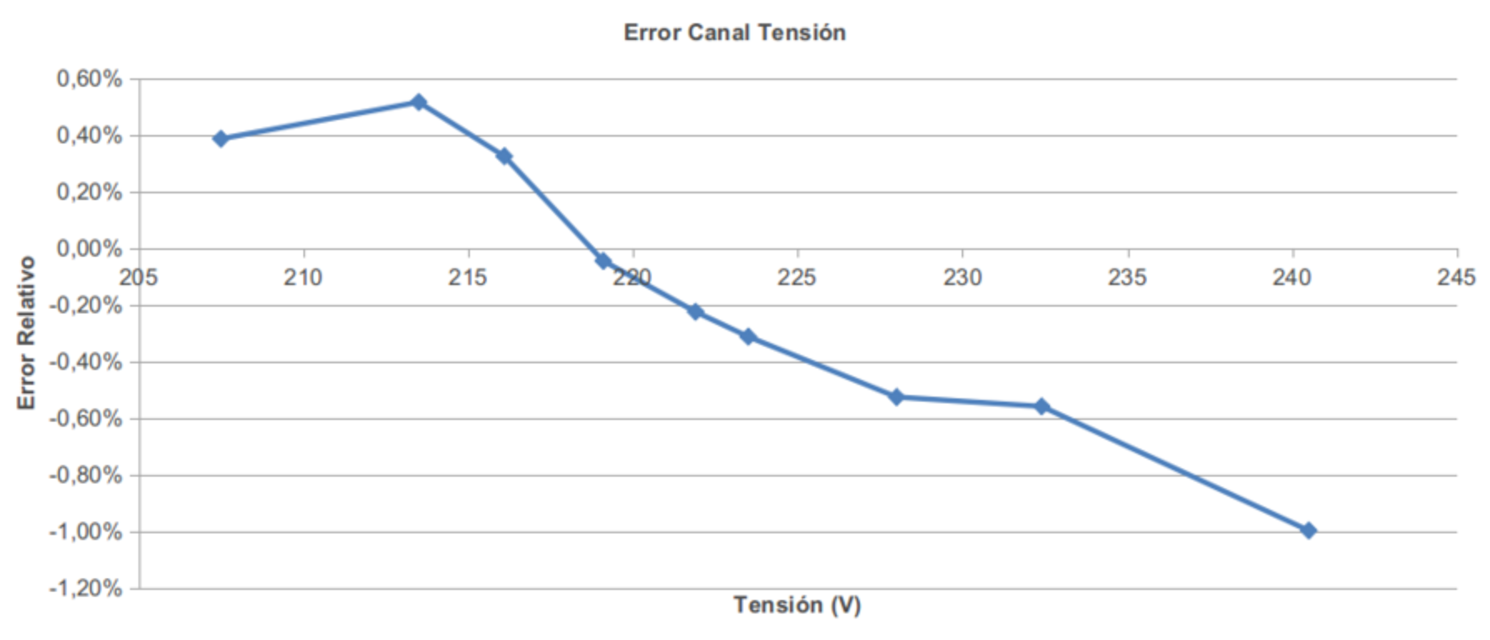
\includegraphics[width=12cm]{./Figures/4_1_1_error_canal_tension.pdf}
	\caption{Error relativo en el canal de tensión.}
	\label{fig:error_canal_tensión}
\end{figure}

\begin{figure}[h]
	\centering
	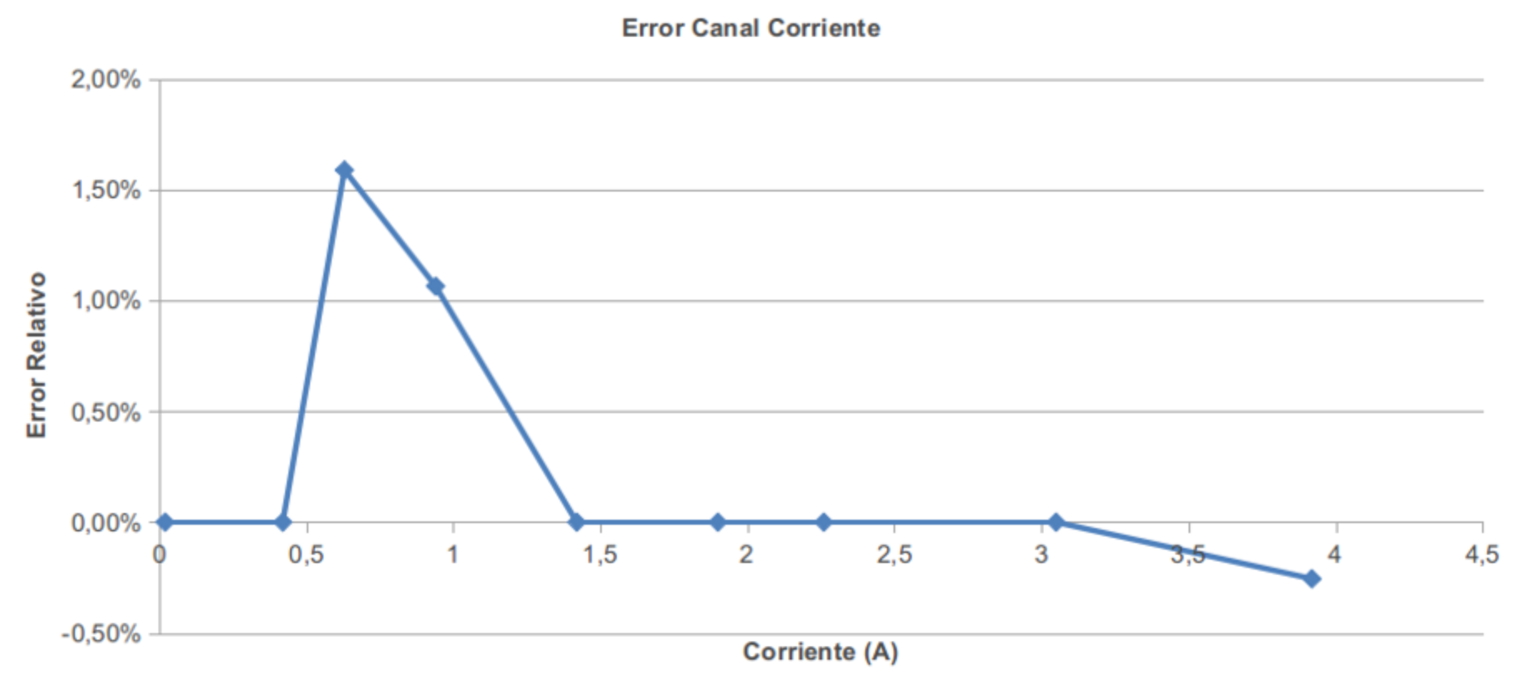
\includegraphics[width=12cm]{./Figures/4_1_1_error_canal_corriente.pdf}
	\caption{Error relativo en el canal de corriente.}
	\label{fig:error_canal_corriente}
\end{figure}

En el caso de la tensión, se utilizó el autotransformador variable para generar distintas tensiones de entrada y se comparó la tensión medida por el Smart Plug contra un voltímetro usado para el contraste. Como puede verse, el error relativo se encuentra por debajo del 1\% en todo el rango de tensión desde los 200VAC hasta los 240VAC.

En el caso de la corriente, se ajustó la tensión de línea sobre el Smart Plug en 10VAC utilizando el autotransformador, y se usaron distintas combinaciones de resistencias de potencia para generar diferentes corrientes. Para contrastar las mediciones se empleó un amperímetro. Los resultados se encuentran por debajo del 2\% en el rango de 0,02A hasta 4A. Los puntos en los que el error relativo está por arriba del 1\% en realidad representan una variación de una centésima en la medición respecto del amperímetro.



\section{Firmware}
\label{sec:validacion_firmware}

En el caso de la validación de los requerimientos del firmware, la totalidad de las pruebas se encuentran descritas en el documento \textit{Smart Plug Firmware - Documento de Pruebas v1.0} en \citep{repo_docu_firmware}.

Uno de los aspectos que se debió validar en el caso del firmware fueron las señalizaciones del led bicolor. Este led es el único medio que tiene el usuario para conocer cómo está funcionando su Smart Plug, por lo que su funcionamiento debe ser confiable. Para generar todas las señalizaciones implementadas se implementaron distintos casos de prueba en los que se simulaba la condición de funcionamiento o de falla y se observaba el resultado en el led.

A continuación se resumen las pruebas para las distintas señalizaciones:

\begin{itemize}
\item Led verde destellante a 2Hz: esta señalización se produce al iniciar el Smart Plug como un punto de acceso. Para esto, se mantuvo presionado el pulsador en la placa del Smart Plug durante 5 segundos y se comprobó que el Plug creara una red WiFi. El led comenzó a destellar con una frecuencia de 2Hz (medido con un osciloscopio) cuando se creó la red WiFi. El led dejó de destellar cuando se configuró una red WiFi a la que se tenía que conectar el Smart Plug.
\item Led verde destellante a 1Hz: esta señalización se produce mientras dura el proceso de WPS. Para producirla, se presionó el pulsador en la placa del Smart Plug. Luego de hacer esto, el led comenzó a destellar con una frecuencia de 1Hz. Se presionó el botón de WPS en un router WiFi y cuando el Smart Plug se unió a la red, el led verde dejó de destellar.
\item Led rojo destellante a 1Hz: se produce cuando el Smart Plug no puede registrarse en una red WiFi. Para producir esta situación se enciende el Smart Plug con el router WiFi desenergizado. Luego de unos segundos, al no poder conectarse a la red WiFi, el led rojo comenzó a destellar a una frecuencia de 1Hz.
\item Led verde y rojo destellan: se produce cuando el Smart Plug no puede sincronizar la su fecha y hora con un servidor NTP. Para producir esta falla, se configuró el router WiFi para que impidiera las conexiones a la dirección IP del servidor NTP usado por el Plug. Cuando se encendió el Smart Plug, luego de unos segundos el led verde y el rojo comenzaron a destellar.
\item Led verde encendido: esta señalización indica el correcto funcionamiento del Smart Plug. Para producir esta situación se eliminaron las condiciones de falla antes simuladas y el led verde se encidió luego de unos segundos.
\end{itemize}


Otro aspecto importante que debió validarse es que el Smart Plug generara un mensaje UDP periódico cada 2 segundos a la dirección de broadcast de la red WiFi. Es importante que estos mensajes existan ya que la aplicación móvil depende de estos para identificar a los Plugs existentes en la red. Además, dentro de estos mensajes periódicos debe informarse el número de ID único del dispositivo.

Para realizar la prueba se tulizó una computadora, dentro de la misma red que el Smart Plug, ejecutando un capturador de paquetes (Wireshark). En la Figura \ref{fig:mensajes_udp} puede verse una porción de la captura, en la que se aprecia que el tiempo entre mensajes UDP dirigidos a la dirección broadcast de la red es de aproximadamente 2 segundos. Además, en la misma figura se puede ver el contenido de uno de los mensajes, en donde se resaltan los seis dígitos del ID del Smart Plug (en este caso 123456) expresado en caracteres ASCII.

\begin{figure}[h]
	\centering
	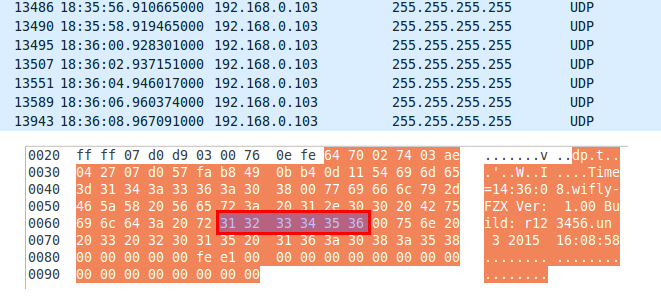
\includegraphics[width=12cm]{./Figures/4_1_2_mensajes_udp.png}
	\caption{Mensajes UDP periódicos recibidos de un Smart Plug, utilizados para identificarlo dentro de la red WiFi.}
	\label{fig:mensajes_udp}
\end{figure}


El protocolo desarrollado para comunicar los Smart Plugs con la aplicación móvil requirió ser validado completamente, probando todos los comandos y registros, para determinar si se producían las acciones esperadas y se devolvían las respuestas debidas.

Para poder conducir las pruebas sin la necesidad de desarrollar la aplicación móvil (la cual no estaba implementada al momentos de llevar a cabo la validación del firmware), se diseño e implementó una aplicación para PC que permitiera generar las tramas de acuerdo a la especificación del protocolo.

En la Figura \ref{fig:simulador_tcp} puede verse una captura del software desarrollado utilizando QT.

\begin{figure}[h]
	\centering
	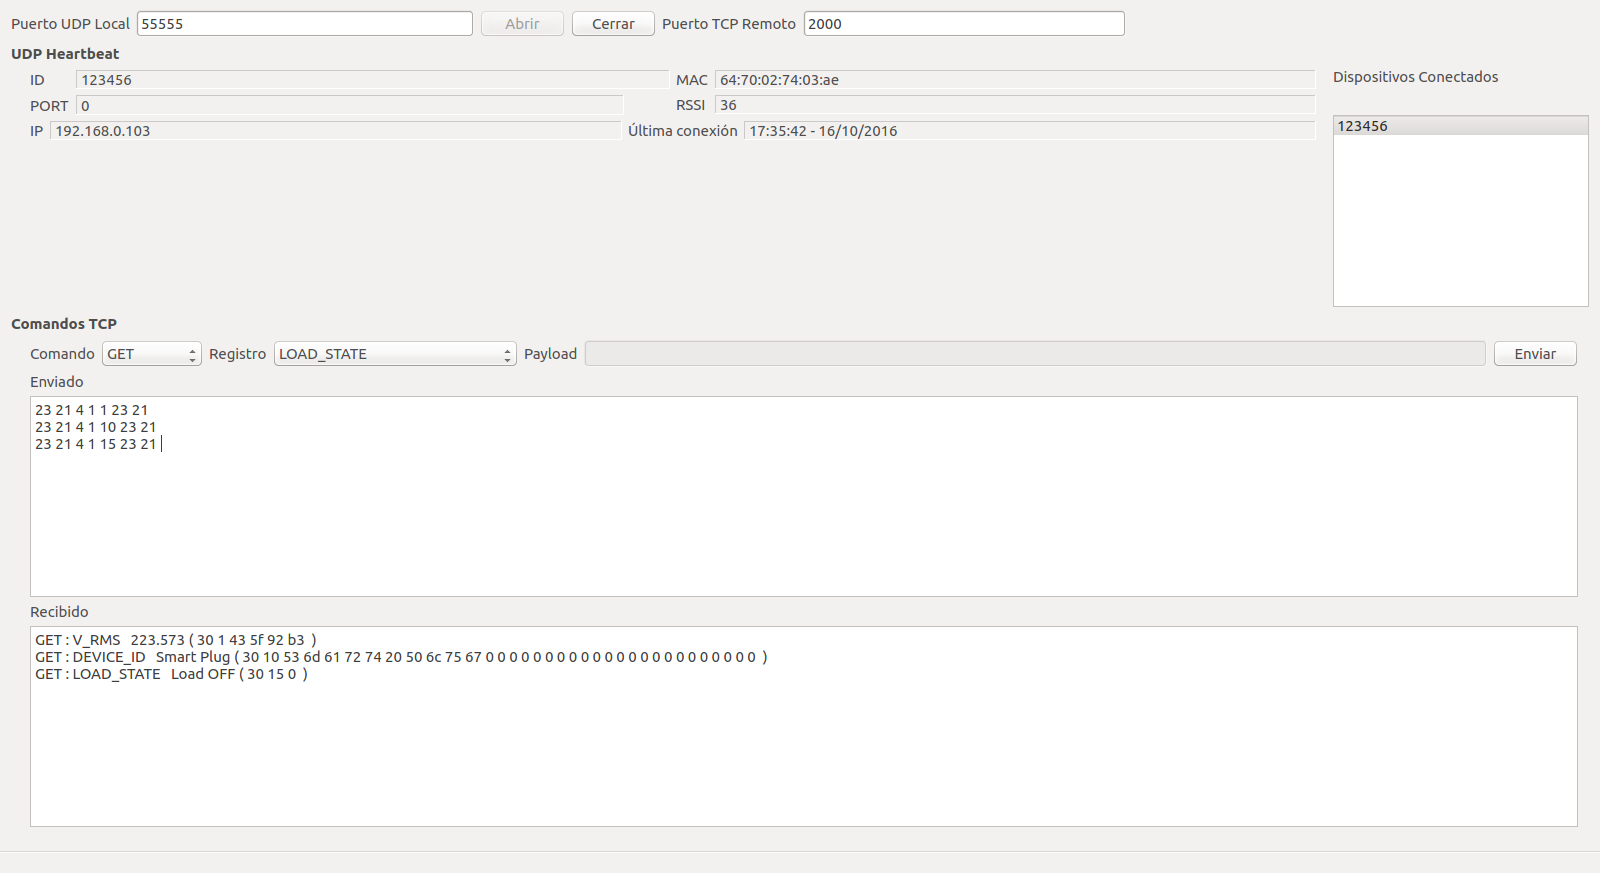
\includegraphics[width=14cm]{./Figures/4_1_2_simulador_tcp.png}
	\caption{Captura del software desarrollado que permite generar todos los comandos propuestos en el protocolo de comunicación.}
	\label{fig:simulador_tcp}
\end{figure}

La interfaz gráfica del software consta de cuatro secciones principales:

\begin{enumerate}
\item Permite elegir el puerto UDP en el que escuchar los mensajes periódicos enviados por los Smart Plugs y el puerto TCP al que mandar las tramas. Los Smart Plugs envían sus mensajes periódicos al puerto UDP 55555 y escuchan las conexiones TCP en el puerto 2000.

\item Cuando se abre el puerto UD, se empiezan a recibir mensajes periódicos de los Smart Plugs que estén conectados en la misma red a la que pertenece la computadora que está corriendo esta aplicación. Cuando llega un mensaje periódico se agrega el ID único del Plug que lo envió en la lista de la derecha, como puede verse con el Plug de ID 123456. Al seleccionar uno de los Smart Plugs de la lista, en los controles de la izquierda de esta sección se visualizarán algunos parámetros del Plug: dirección AMAC, IP, RSSI de la señal WiFi, hora de llegada del mensajes, etc.

\item Esta sección permite elegir el comando que se va a enviar al Smart Plug seleccionado en la sección 2. Se debe elegir tanto el comando como el registro afectado (en caso de que corresponda). Además, si el comando requiere un parámetro adicional, como puede ser el en el caso del comando SET, en el campo Payload se puede ingresar los datos que debe llevar la trama.

\item Muestra la trama enviada y la trama recibida como respuesta. En el caso de la respuesta. se muestra la misma parseada de acuerdo al comando y al registro manipulado. De esta forma, si se está enviando el comando GET de un registro de tipo float, la aplicación mostrará el contenido de la respuesta como un float.
\end{enumerate}

Utilizando esta aplicación se llevaron a cabo numerosos casos de prueba para comprobar la correcta implementación del protocolo en el firmware del Smart Plug. Tanto las pruebas como los resultados obtenidos pueden verse en el documento \textit{Smart Plug Firmware - Documento de Pruebas v1.0} en \citep{repo_docu_firmware}.

El código fuente de esta aplicación se encuentra en \citep{repo_simulador_tcp}.


\section{Aplicación móvil}

En el caso de la aplicación móvil, además de las pruebas de caja negra para validar sus requerimientos (las cuales pueden encontrarse en el documento \textit{Smart Plug App - Documento de Pruebas v1.0} en \citep{repo_docu_app}) se llevó a cabo una prueba general del sistema para comprobar su funcionamiento.

Básicamente la prueba general consistió en dejar conectado el Smart Plug durante 5 días con una lámpara de 60W conectada y se realizaron distintas configuraciones para comprobar su funcionamiento.

Las acciones que se realizaron dentro de la prueba fueron:

\begin{itemize}
\item Configuración de la programación horaria para algunos días de la semana.
\item Encendido y apagado de la carga mediante la aplicación.
\item Comprobación de las mediciones eléctricas.
\item Visualización de los gráficos de potencia y energía consumida por hora.
\end{itemize}

Mediante la programación horaria se pudo comprobar que la carga se encendía y apagaba de acuerdo al día de la semana y a las horas configuradas para ese día.

Presionando el ícono asociado al Smart Plug en la lista de Plugs encontrados se pudo encender y apagar la carga.

Luego de pasados los 5 días se tenían 5 gráficos históricos de potencia y de energía consumida como se ve en la Figura \ref{fig:integracion}. En la parte derecha de la figura, puede verse uno de los gráficos de potencia promedio por hora.


\begin{figure}[h]
	\centering
	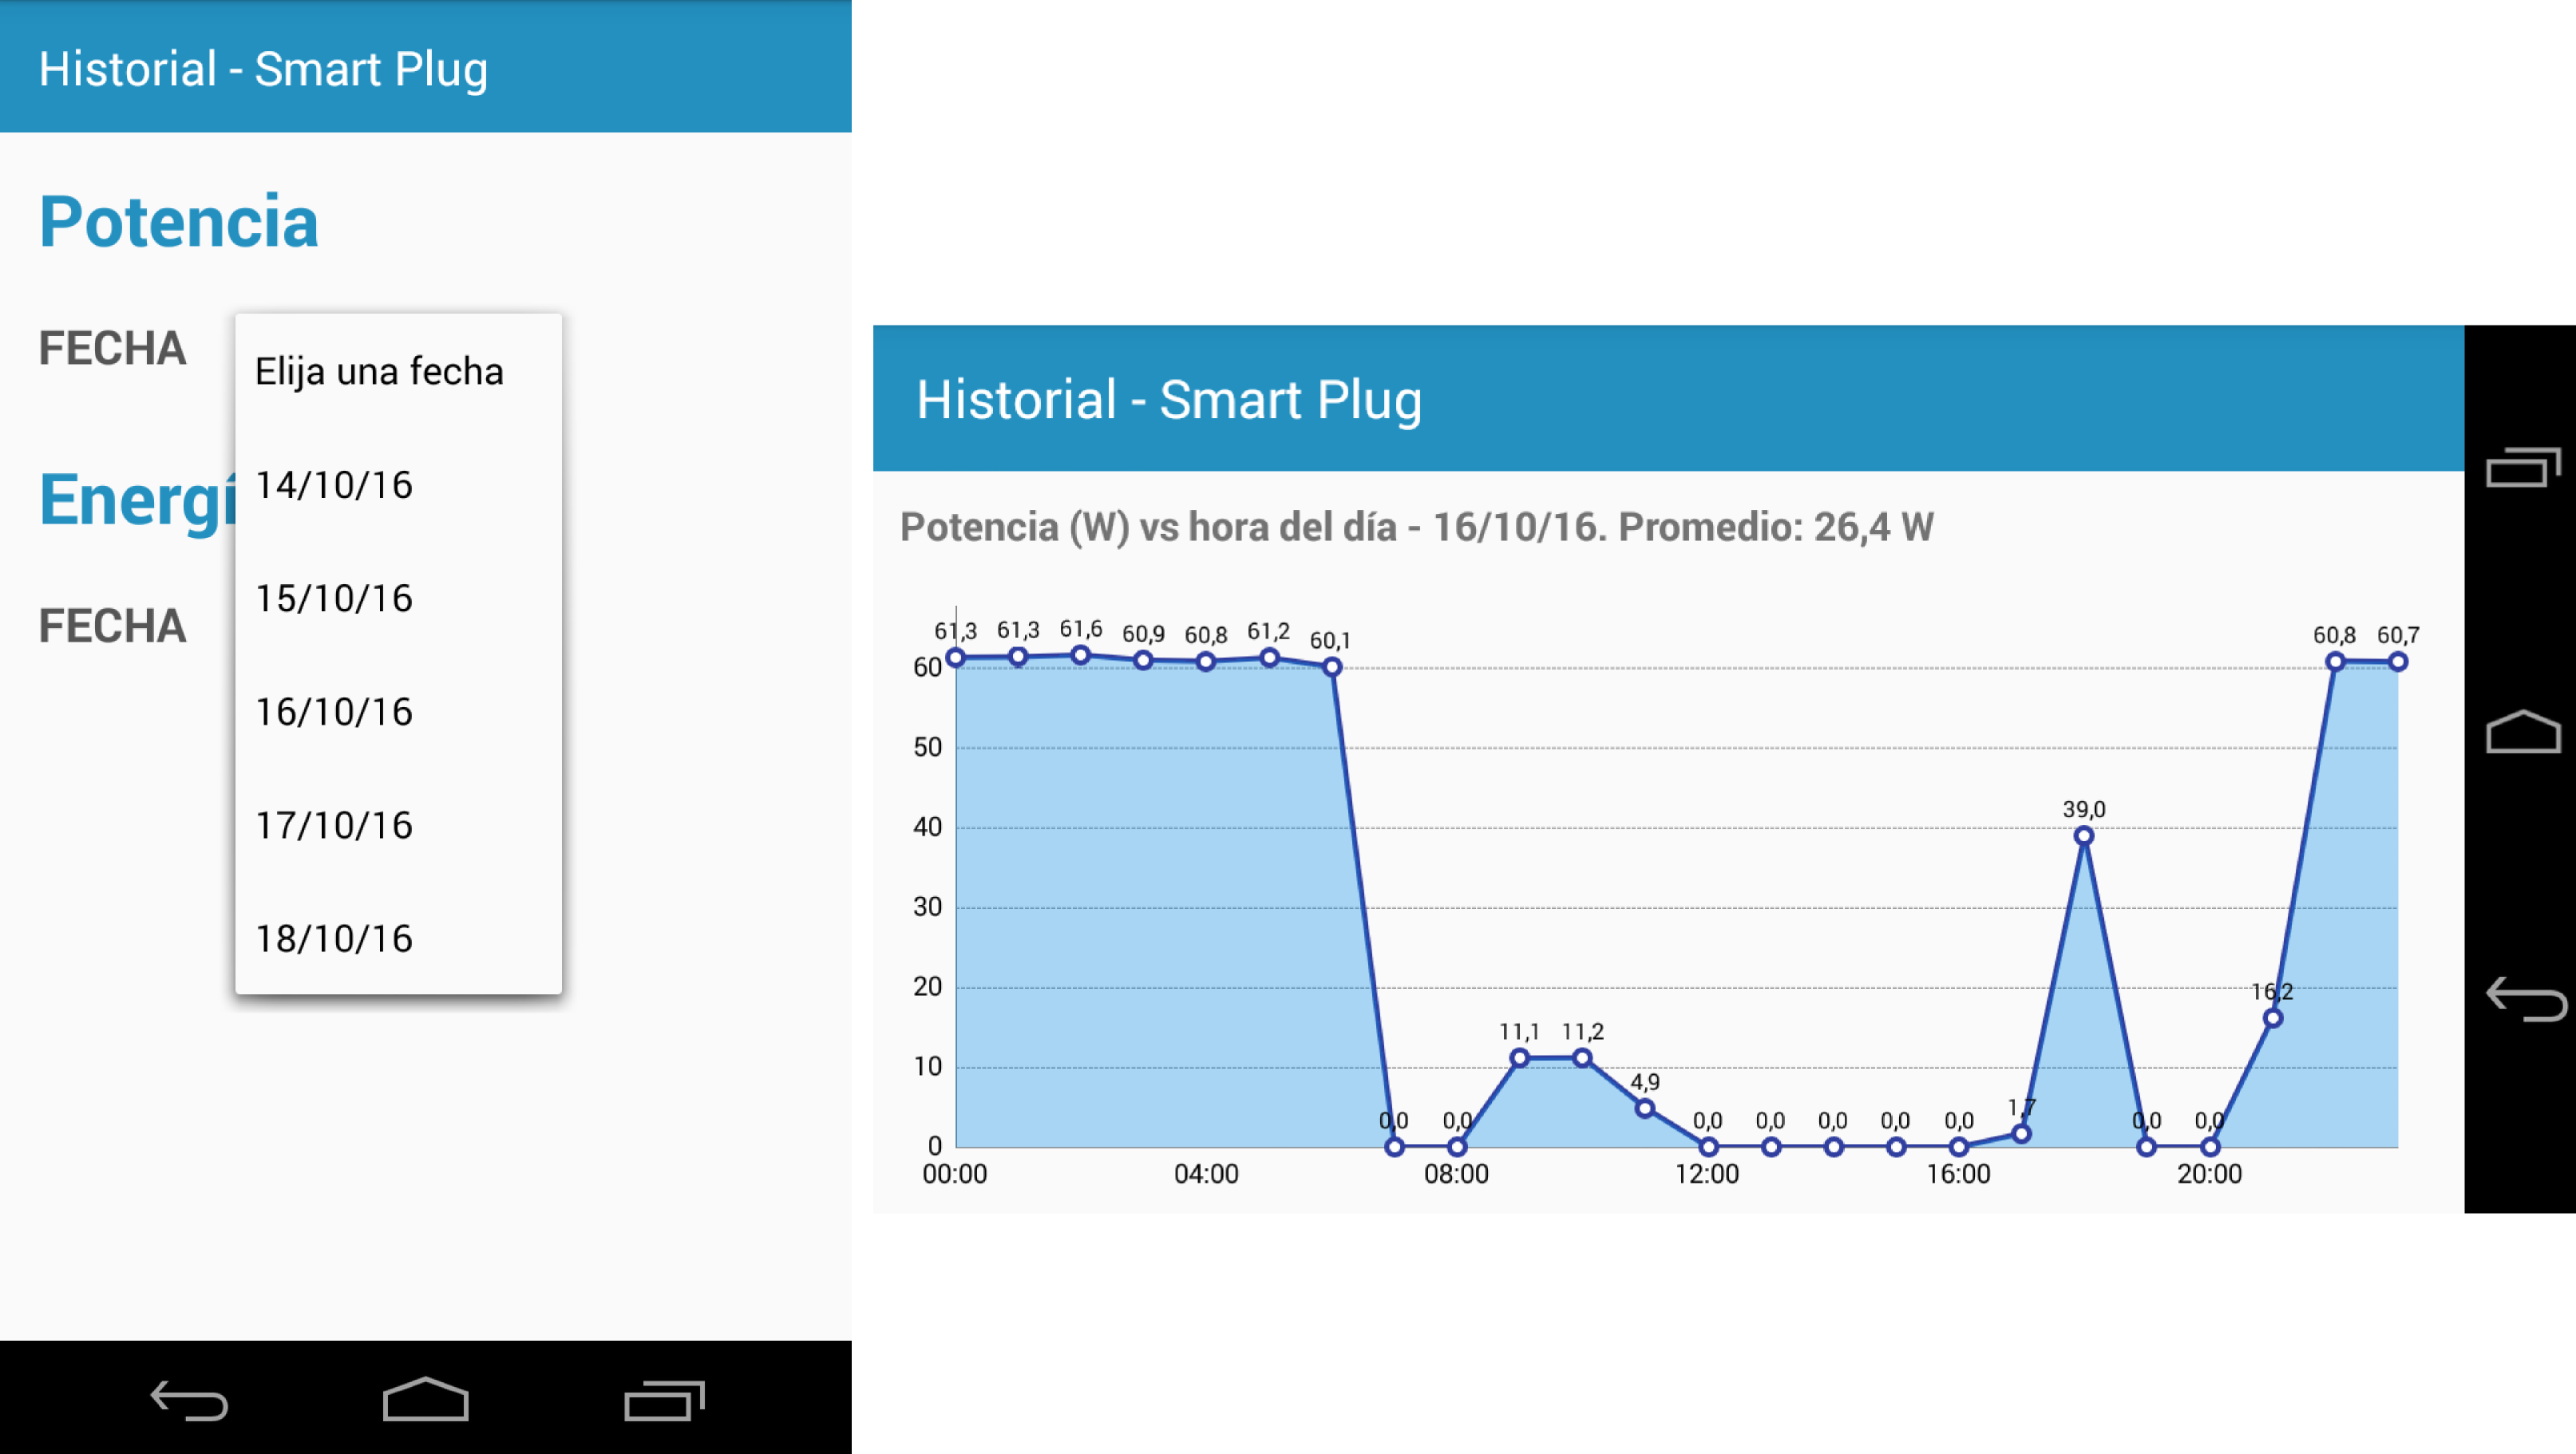
\includegraphics[width=12cm]{./Figures/4_1_3_integracion.png}
	\caption{Capturas de la aplicación móvil resultantes de la prueba de funcionamiento general del Smart Plug.}
	\label{fig:integracion}
\end{figure} 
% Chapter Template

\chapter{Conclusiones} % Main chapter title

\label{Chapter5} % Change X to a consecutive number; for referencing this chapter elsewhere, use \ref{ChapterX}

En este capítulo se presentan las principales conclusiones del trabajo, así como también las futuras mejoras que se pueden realizar sobre el equipo.


\section{Conclusiones generales}

En la presente memoria se documentó el diseño e implementación de un Smart Plug. Se logró construir un prototipo funcional que permitió evaluar las prestaciones del equipo y desarrollar una aplicación para dispositivos móviles con sistema Android para poder interactuar con los Smart Plugs. 

La información provista por cada uno de los Plugs le permitirá al usuario conocer el consumo de los dispositivos eléctricos, ayudándolo a tomar decisiones con el objetivo de cambiar la forma en que los utiliza. Se tomó como principal objetivo en el diseño de la aplicación, que la misma fuera sencilla de utilizar y que presentara los datos de una forma útil.

El dispositivo desarrollado será uno de los primeros equipos de fabricación nacional con estas características, complementando la línea de productos de domótica ya existente.

Para la realización del proyecto se aplicaron los conocimientos aprendidos en la carrera de especialización en sistemas embebidos, principalmente de las siguientes asignaturas:

\begin{itemize}
\item Arquitectura de microprocesadores: en la misma se aprendió la arquitectura del microcontrolador utilizado en el Smart Plug y técnicas básicas de programación. Fue la base para empezar a usar dichos microcontroladores.
\item Programación de microprocesadores: se aplicaron las metodologías aprendidas, el uso de capas para generar abstracción con el hardware y la teoría de programación orientada a objetos.
\item Ingeniería de software en sistemas embebidos: se aplicaron los conocimientos adquiridos para diseñar, implementar y probar tanto el firmware como la aplicación móvil. Esto constituyó uno de los principales aportes del proyecto a la metodología habitual de trabajo, ya que permitirá utilizar las técnicas y herramientas aprendidas a otros desarrollos.
\item Gestión de Proyectos en Ingeniería: lo aprendido en esta asignatura permitió abordar el proyecto de forma ordenada, previendo las tareas  que se debían realizar y el tiempo que se le debía dedicar a cada una de estas. Tanto las herramientas como la forma de trabajo aprendidas en la materia son otro de los aportes del proyecto a la forma de trabajo habitual.
\item Sistemas Operativos de Tiempo Real: a pesar de que cuando se cursó esta materia, se enseñaba únicamente el uso de FreeRTOS, los conocimientos aprendidos permitieron entender, sin mayores dificultades, el uso de otro RTOS como es FreeOSEK.
\item Protocolos de comunicación en sistemas embebidos: se utilizó la comunicación SPI aprendida en la asignatura.
\item Diseño para manufacturabilidad: se discutieron los diseños y se realizaron revisiones y modificaciones para mejorar el funcionamiento del equipo.
\end{itemize}


Por otro lado, durante el desarrollo de este proyecto, se adquirieron conocimientos en las áreas de:

\begin{itemize}
\item Diseño de aplicaciones móviles: se aprendió la importancia del uso de maquetas al momento de diseñar una aplicación, lo cual facilita la articulación entre la estética buscada y la funcionalidad de la aplicación.
\item Programación de aplicación para el sistema Android: a pesar de que que se contaba con alguna experiencia en programación de aplicaciones bajo Android, la aplicación desarrollada introdujo el uso de nuevas clases, especialmente relacionadas con el manejo de servicios.
\end{itemize}


\section{Trabajo futuro}
\label{sec:trabajo_futuro}

Para continuar con el desarrollo del equipo, con el objetivo de obtener un producto comercial, se plantearon las siguientes mejoras y modificaciones sobre las que se debe trabajar:

\begin{itemize}
\item Rediseñar la adaptación de las señales de tensión y corriente para reducir el tamaño del PCB. Evaluar la posibilidad de utilizar divisores resistivos para el canal de tensión y un shunt para la corriente. Implementar un diseño propio de fuente switching la cual se integre en el PCB del producto.
\item Agregar la lógica del proceso de prueba en fábrica. La comunicación entre el probador del equipo y el equipo se realizará a través de la UART de debug, por lo que se debe modificar la tarea moduleLog para permitir recibir comandos durante la prueba. La prueba de fábrica incluirá: grabación del ID único, calibración de continua y de ganancia del canal de corriente y de tensión del front-end analógico.
\item En la aplicación móvil, el agregado de un nuevo Smart Plug se realizará introduciendo el ID único del producto. En la versión descrita en este trabajo, la aplicación muestra todos los Smart Plugs que encuentra.
\item En la aplicación móvil, se agregará información acerca del costo de la energía consumida y se introducirá la posibilidad de configurar un nivel de energía o de dinero, superado el cual se generarán notificaciones en el celular.
\item Desarrollar la infraestructura necesaria para permitir comandar los Smart Plugs tanto desde la misma red WiFi en la que se encuentran como desde cualquier otra red.
\end{itemize}

 

%----------------------------------------------------------------------------------------
%	APÉNDICES
%----------------------------------------------------------------------------------------

\appendix % indicativo para indicarle a LaTeX los siguientes "capítulos" son apéndices

% Incluir los apéndices de la memoria como archivos separadas desde la carpeta Appendices
% Descomentar las líneas a medida que se escriben los apéndices

%% Appendix A

\chapter{Appendix Title Here} % Main appendix title

\label{AppendixA} % For referencing this appendix elsewhere, use \ref{AppendixA}

Write your Appendix content here.
%\include{Appendices/AppendixB}
%\include{Appendices/AppendixC}

%----------------------------------------------------------------------------------------
%	BIBLIOGRAPHY
%----------------------------------------------------------------------------------------

\Urlmuskip=0mu plus 1mu\relax
\raggedright
\printbibliography[heading=bibintoc]

%----------------------------------------------------------------------------------------

\end{document}  
